\documentclass{base}

% 设置页眉
\usepackage{fancyhdr}
\pagestyle{fancy}
\fancyhead{} % 清除默认页眉
\fancyhead[C]{\textcolor{gray}{工程项目开发综合实践课程论文}} % 中间位置

% 使图片按照章节编号
\usepackage{amsmath}
\numberwithin{figure}{section} %关联图号和章节,应该是每一个section重置一下图号计数器

% 使表格按照章节编号
\usepackage{caption}
\usepackage{chngcntr} % 为了使用 \counterwithin 命令
\counterwithin{table}{section} % 将表格编号与 section 关联

% 额外包
\usepackage{booktabs}
\usepackage{longtable}
\usepackage{graphicx}
\usepackage{subcaption}
\usepackage{pdfpages}
\usepackage{xcolor}

% 全文双倍行距
\doublespacing

\begin{document}

% 封面
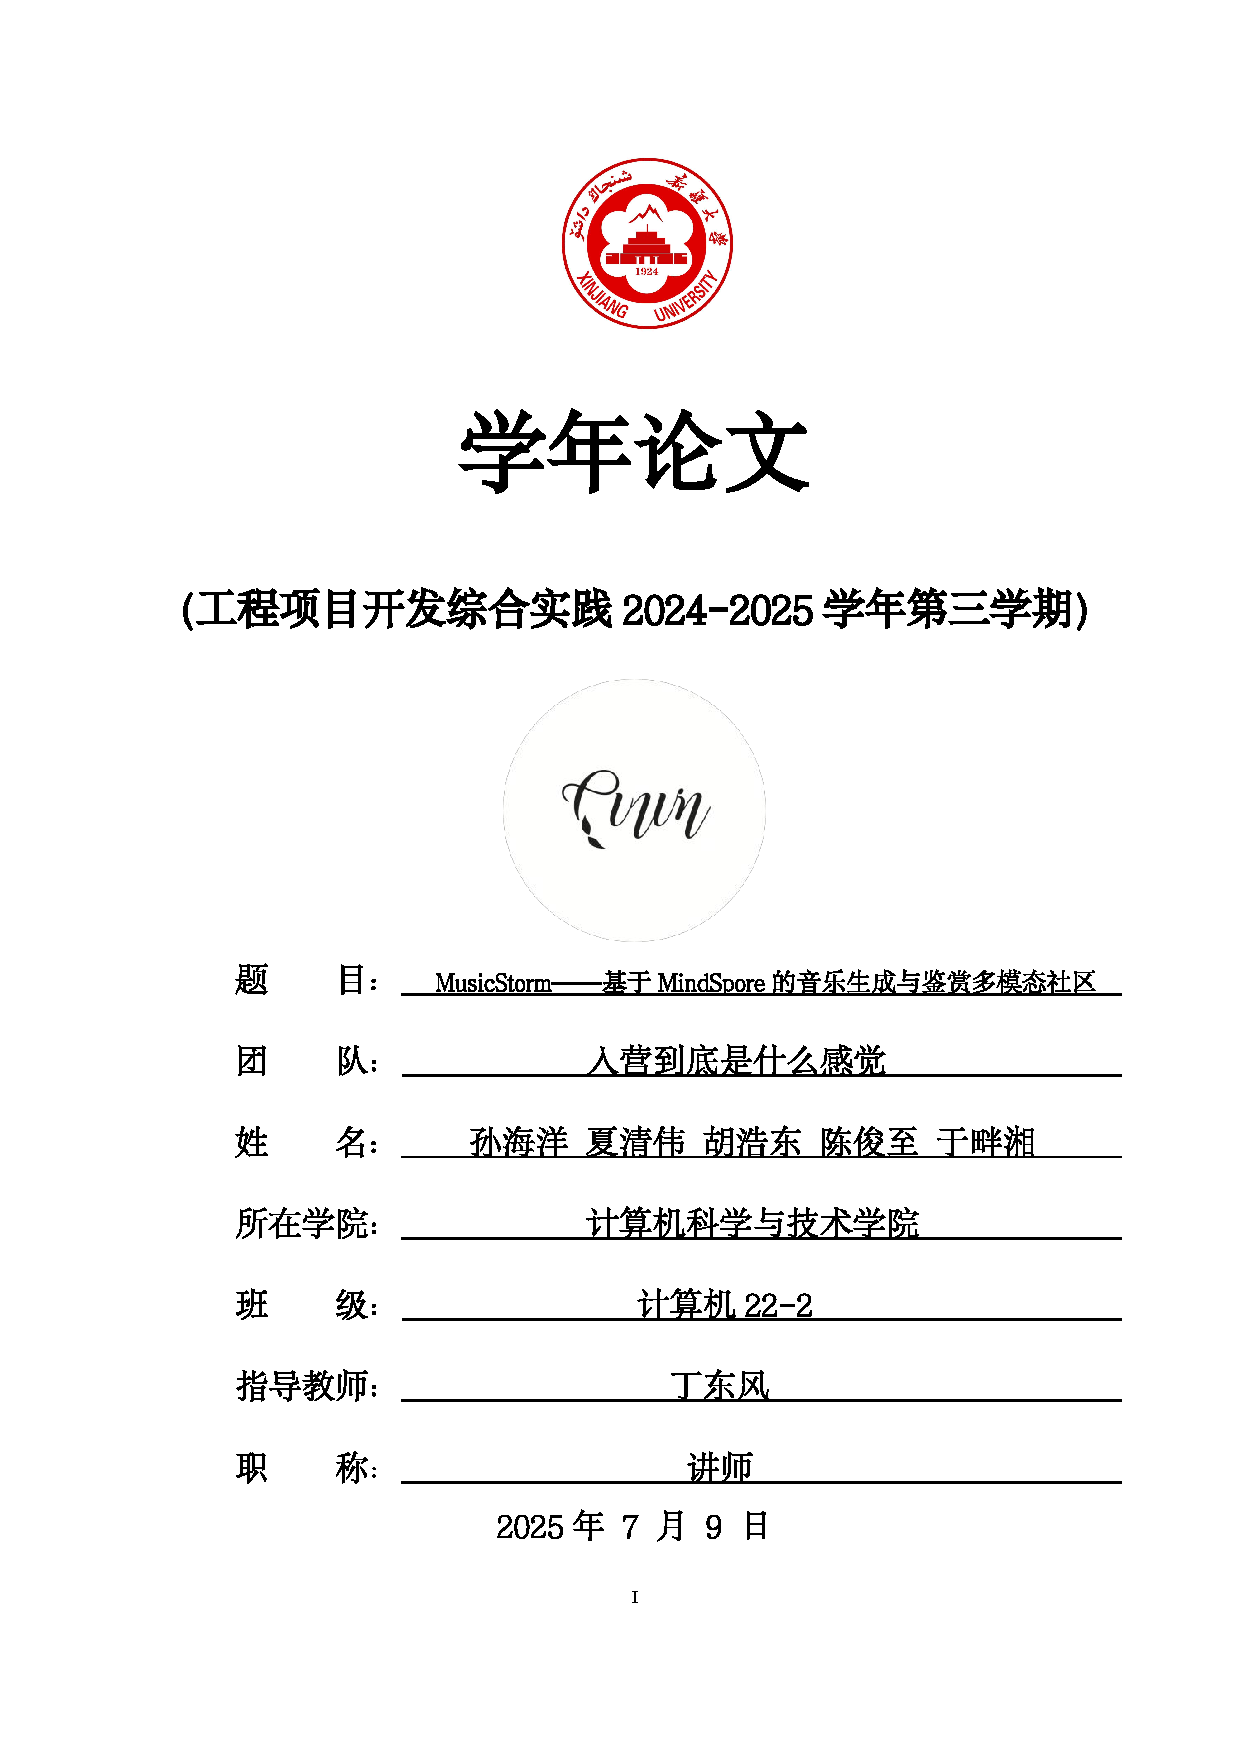
\includepdf[pages=-]{otherpdf/cover.pdf}

\tableofcontents

\newpage

\section{引言}

\subsection{开发目的}

本软件(以下均简称MS)旨在为 Android 用户提供一个集AI音乐创作,作品分享,音乐鉴赏,社区互动为一体的音乐社区平台。

\subsection{现状及意义}

随着信息时代的逐渐发展,AI创作以及普及到了世界各地。早在2023年,Google已经发布了MusicLM,它能够根据用户输入的文字描述(如风格、情绪、乐器、场景等),直接生成高质量、结构完整的音乐片段(最长可达数分钟),标志着 AI 音乐生成技术的重要突破。然而当前国内市场上未存在“AI创作+鉴赏交流”的社交平台。
本软件可以推动多模态AI音乐技术落地,融合生成、编辑、分析能力,实现从"工具"到"创作伙伴"的升级。打破音乐创作阶层壁垒,促进多元文化表达,为独立音乐人提供新舞台。通过社区乐评、风格解析等功能,提升大众音乐素养,传承音乐文化。

\subsection{背景}

为了为众多音乐爱好者提供良好便捷的交流以及自主编写音乐的平台,我们小组决定开发一个音乐生成及鉴赏社区。该项目由我们小组组长提出,由小组成员共同完成。面向群众为音乐爱好者,独立音乐人,音乐教育者等人群。本项目使用华为昇腾MindSpore框架,私有化部署AI模型进行增量化模型训练。

\newpage

\section{系统可行性分析}
\subsection{可行性研究的前提}
\subsubsection{要求}

\textbf{A. 功能}

\textbf{音乐生成功能}\quad 基于 MindSpore 框架,接收文本、图像等多模态输入,实现流行、古典、电子等多风格音乐的自动生成,支持用户对生成音乐的节奏、旋律、和声等参数进行个性化调整。

\textbf{音乐鉴赏功能}\quad 通过人工智能技术分析音乐的旋律结构、和声走向、节奏特点等元素,结合用户评价与社区互动数据,为用户提供音乐评分、优缺点分析、相似音乐推荐等鉴赏服务。​

\textbf{社区交互功能}\quad 构建用户注册登录、作品上传分享、评论点赞、私信交流、关注粉丝等社交功能,打造音乐创作者与爱好者交流互动的平台,支持用户创建或加入音乐主题小组。

\textbf{B. 性能}

\textbf{响应时间}\quad 音乐生成请求在普通网络环境下,响应时间不超过 12 秒;社区交互操作如评论、点赞等,响应时间控制在 1.5 秒以内。

\textbf{吞吐量}\quad 支持至少千级用户同时在线访问,每秒可处理 500次以上的音乐生成与社区交互请求。

\textbf{稳定性}\quad 系统全年可用性不低于 99.9\%,平均无故障运行时间(MTBF)不低于5000小时,具备自动容灾与故障恢复能力。

\textbf{C. 输出}

\textbf{生成音乐文件}\quad 格式为常见的 MP3、WAV 等,用于用户下载保存、分享传播,每次音乐生成操作即产生,用户可通过社区平台下载接口获取,分发对象为音乐生成的用户及该用户分享的其他社区成员。

\textbf{音乐鉴赏报告}\quad 以文字、图表结合的形式,展示音乐的各项分析数据与评价结果,在用户触发鉴赏功能时生成,可在线查看或下载为 PDF 格式,接口位于音乐作品详情页,分发对象为发起鉴赏请求的用户。​

\textbf{社区数据统计报表}\quad 按日、周、月统计用户活跃度、作品上传数量、社区互动数据等,用于项目运营分析,产生频度为每周,以 Excel 格式存储,通过后台管理系统接口获取,分发对象为项目运营团队。

\textbf{D. 输入}

\textbf{数据来源}\quad 音乐生成的多模态输入数据来源于用户手动输入;音乐鉴赏的原始音乐数据由用户上传及合作音乐平台授权提供;社区交互数据来自用户在平台的操作行为。​

\textbf{数据类型}\quad 包括文本(用户输入的描述、评论等)、图像(作为音乐生成灵感的图片)、音频(用户上传的音乐作品、待鉴赏的音乐)、用户操作日志等数据类型。​

\textbf{数据数量与组织}\quad 预计初期每日新增用户输入数据500条左右,音乐文件上传量100个,随着用户增长逐步上升;数据按用户 ID、功能模块进行分类存储与管理,采用分布式数据库架构。

\textbf{提供频度}\quad 用户输入数据实时产生;音乐文件上传与社区交互数据持续产生;合作平台提供的音乐数据根据合作协议定期更新。

\textbf{E. 安全与保密方面要求}

\textbf{数据安全}\quad 采用加密技术对用户上传的音乐文件、个人隐私数据进行加密存储与传输,防止数据泄露;定期进行数据备份,确保数据的完整性与可恢复性。​

\textbf{用户认证与授权}\quad 严格用户注册登录认证机制,采用账号密码、手机验证码、第三方平台授权等多种认证方式;对用户操作权限进行分级管理,不同权限用户只能访问相应功能与数据。​

\textbf{系统安全防护}\quad 部署防火墙、入侵检测系统等安全防护设备,实时监测系统安全状态,防范网络攻击、恶意访问等安全威胁。

\subsubsection{目标}

\textbf{A. 人力与设备费用的减少}

通过 MindSpore 框架的高效性与自动化特性,降低音乐生成与鉴赏算法开发过程中对人力的依赖。利用框架内置的模型训练与优化功能,减少开发人员手动调参、代码优化的工作量,缩短开发周期,进而降低人力成本。MindSpore 的分布式训练与推理能力,可有效提升服务器资源利用率,避免因资源浪费而额外购置设备,降低硬件设备投入费用,实现人力与设备资源的高效配置。

\textbf{B. 处理速度的提高}

借助 MindSpore 强大的计算能力与优化算法,提升音乐生成与鉴赏系统的处理速度。在音乐生成环节,针对用户输入的多模态数据,系统可快速调用预训练模型进行分析与生成,确保在普通网络环境下,音乐生成请求响应时间不超过 8 秒。对于音乐鉴赏功能,通过对音乐元素的并行分析与智能算法优化,结合社区互动数据的快速检索,能在短时间内生成音乐鉴赏报告,同时保证社区交互操作如评论、点赞等响应时间控制在1.5秒以内,为用户提供流畅高效的使用体验。

\textbf{C. 管理信息服务的改进}

MusicStorm 社区通过整合用户行为数据、音乐作品数据、社区互动数据等多维度信息,构建完善的管理信息服务体系。运营团队可通过后台管理系统实时获取用户活跃度、作品上传数量、社区互动趋势等统计报表,以周为周期生成详细的数据分析报告。这些数据支持可视化展示与深度挖掘,帮助运营团队更精准地了解用户需求、评估社区运营效果,从而制定更有效的运营策略,实现管理信息服务从传统人工统计向智能化、精准化的转变。

\subsubsection{条件、假定和限制}

\textbf{A. 所建议系统的运行寿命的最小值​}

假定 MusicStorm 系统的运行寿命最小值为2年。在这期间,需持续维护系统的稳定性与功能性,不断进行技术迭代与优化,以适应市场变化与用户需求升级,确保系统在音乐生成、鉴赏及社区交互等核心功能上保持竞争力,同时保障用户数据安全与服务质量。

\textbf{B. 进行系统方案选择比较的时间​}

在项目启动后的第2天内,完成系统方案的选择与比较工作。此阶段将综合评估不同技术方案在实现音乐生成、鉴赏及社区交互功能上的可行性、效率、成本等因素,结合 MindSpore 框架特性,确定最优开发方案,为后续开发工作奠定基础,避免因方案选择延误项目整体进度。

\textbf{C. 法律和政策方面的限制​}

\textbf{音乐版权法律}\quad 在音乐生成、上传、分享及传播过程中,需严格遵守《著作权法》等相关法律法规,确保用户上传作品的版权合法性,以及生成音乐的版权归属明确。对于用户生成内容(UGC),需建立完善的版权审核与授权机制,避免侵权纠纷。​
互联网信息服务政策:遵循国家互联网信息服务相关规定,对社区内容进行严格审核与管理,禁止出现违法违规、低俗有害信息。定期进行内容合规性检查,及时响应政策变化,调整运营策略,确保系统合法合规运营。

\textbf{D. 可利用的信息和资源​}

\textbf{数据资源}\quad 可利用公开的音乐数据集(如 MIR - 1K、GTZAN 等)进行模型训练与优化,同时与音乐版权方、流媒体平台合作,获取授权音乐数据用于鉴赏功能。此外,社区用户生成的内容与交互数据将成为重要的数据资源,用于改进系统功能与用户体验。​
技术资源:依托 MindSpore 社区的技术文档、开源模型及开发者支持,加速项目开发进程。同时,借鉴人工智能、音乐信息检索等领域的前沿研究成果,提升系统技术水平。

\subsubsection{进行可行性研究的方法}

\textbf{A. 技术可行性研究方法​}

\textbf{文献研究与技术调研}\quad 广泛查阅国内外关于 MindSpore 框架应用、音乐生成算法、多模态数据处理及社区平台开发的学术文献、技术报告和行业案例。重点分析 MindSpore 在音乐领域的成功实践,研究当前主流音乐生成模型(如变分自编码器 VAE、生成对抗网络 GAN 在音乐生成中的应用)的优缺点,了解多模态数据融合技术的发展现状,为项目技术方案提供理论支撑与技术参考。​

\textbf{技术测试与实验}\quad 搭建小型技术验证平台,针对 MusicStorm 的核心功能进行技术测试。例如,基于 MindSpore 框架实现简单的音乐生成模块,测试其在不同风格音乐生成上的效果;开发初步的多模态输入接口,验证文本、图像等数据转换为音乐元素的可行性与准确性;构建基础的社区交互原型,测试系统在高并发访问下的性能表现。通过实验数据评估技术方案的可行性与潜在风险。

\textbf{B. 社会可行性研究方法}

\textbf{法律与政策合规性审查}\quad 全面梳理与音乐产业、互联网服务相关的法律法规与政策文件,确保 MusicStorm 项目在音乐版权管理、用户数据保护、内容审核等方面符合法律要求。定期关注政策变化,及时调整项目运营策略,避免法律风险,保证项目的合法合规运营。​
\textbf{社会影响评估}\quad 分析项目对音乐产业生态、社会文化发展的影响。评估项目是否有助于推动音乐创作创新、促进音乐文化传播、培养音乐人才;研究项目对社会就业、经济增长的贡献,判断项目在社会层面的可行性与价值。​
\textbf{利益相关者分析}\quad 识别项目的利益相关者,包括用户、音乐版权方、投资者、合作伙伴等,分析各利益相关者的需求与期望,评估项目对他们的影响。通过建立良好的沟通机制与合作模式,协调各方利益,确保项目得到社会各界的支持与认可。​

\subsubsection{评价尺度}

\textbf{A. 各项功能的优先次序​}

\textbf{核心功能优先}\quad 音乐生成与鉴赏功能作为项目的核心,优先保证其稳定性与创新性。在开发资源分配上,将 60\%-70\% 的人力和时间投入到核心功能的研发与优化中,确保生成音乐的质量达到专业水准,鉴赏结果具有权威性和参考价值。​
\textbf{基础功能完善}\quad 社区交互功能是用户参与和使用项目的基础,在核心功能开发的同时,同步完善用户注册登录、作品上传分享、评论点赞等基础交互功能,投入 20\%-30\% 的资源,保障社区的基本使用体验。​
\textbf{增值功能拓展}\quad 在核心功能和基础功能稳定运行后,利用剩余 10\%-20\% 的资源,逐步开发会员专属服务、音乐版权交易等增值功能,提升项目的商业价值和用户粘性。

\textbf{B. 开发时间的长短​}

\textbf{计划时间对比}\quad 以项目制定的 12 个月开发周期为基准,在项目开发过程中,定期检查各阶段任务的完成进度。若实际开发时间与计划时间偏差在 ±10\% 以内,视为项目进度可控;若超过 10\%,则需分析原因,判断是技术难题、资源不足还是管理问题导致,并及时调整开发计划。​
\textbf{市场机遇考量}\quad 考虑到音乐市场和人工智能技术的快速发展,若项目开发时间过长,可能错失市场机遇。因此,即使项目在技术上可行,但开发时间超过 15 个月,且市场竞争格局已发生重大变化,也需重新评估项目的必要性和可行性。

\textbf{C. 使用中的难易程度}

\textbf{界面设计友好性}\quad 通过用户测试和问卷调查,评估系统界面的布局是否简洁明了,操作流程是否清晰易懂。若80\%以上的用户认为界面友好,操作方便,则说明系统在界面设计方面表现良好;若低于60\%,则需对界面进行优化改进。​
\textbf{学习成本高低}\quad 观察新用户在首次使用系统时,掌握核心功能所需的时间。若用户能在10分钟内独立完成音乐生成或鉴赏的基本操作,且在30分钟内熟悉社区的主要交互功能,说明系统的学习成本较低,易于使用;反之,则需优化功能设计,降低学习门槛。
\textbf{用户反馈与投诉率}\quad 统计用户在使用过程中的反馈意见和投诉数量,若每月用户投诉率低于0.5\%,且积极反馈建议较多,说明用户对系统的使用体验较为满意;若投诉率超过 1\%,则需深入分析问题根源,及时解决用户痛点,提升系统易用性。
\subsection{对现有系统的分析}

\subsubsection{处理流程和数据流程}

\textbf{A. 处理流程}

音乐生成处理流程:

\begin{enumerate}
    \item 用户在系统界面输入多模态信息,如描述音乐风格、情绪的文本,或上传作为灵感来源的图像等。
    \item 输入数据进入预处理模块,对文本进行语义分析、关键词提取,对图像进行特征识别与转换,将多模态数据转化为适合音乐生成模型处理的格式。​
    \item 数据传输至基于 MindSpore 搭建的音乐生成模型,模型依据预设算法和训练参数,结合输入数据生成音乐的旋律、和声、节奏等元素,形成初步音乐片段。​
    \item 初步生成的音乐片段进入优化调整模块,用户可在此对音乐的速度、调式、乐器音色等参数进行手动调整,系统根据用户指令对音乐片段进行优化。​
    \item 优化后的音乐文件经格式转换,以常见的 MP3、WAV 等格式存储至系统服务器,并返回生成成功提示,用户可选择下载或直接在社区分享。
\end{enumerate}

音乐鉴赏处理流程:

\begin{enumerate}
    \item 用户上传待鉴赏的音乐文件或选择社区内其他用户分享的音乐。​
    \item 音乐文件进入音频解析模块,提取音乐的旋律、和声、节奏、音色等基础音频特征。
    \item 提取的音频特征数据与系统音乐知识库中的标准数据进行比对分析,同时结合社区内其他用户对该音乐的评价数据、点赞收藏数据等进行综合评估。​
    \item 基于分析评估结果,生成包含音乐评分、优缺点分析、相似音乐推荐等内容的鉴赏报告,展示在音乐作品详情页面供用户查看。
\end{enumerate}

社区交互处理流程:​

\begin{enumerate}
    \item 用户注册登录系统,完成身份验证后进入社区。​
    \item 用户可进行作品上传、发布动态、评论他人作品、点赞收藏、关注其他用户、加入主题小组等交互操作。​
    \item 系统实时接收用户交互操作指令,将相关数据存储至用户行为数据库,同时更新社区页面展示内容,如在用户个人主页更新作品列表,在动态信息流展示新发布内容,向被评论、被关注用户发送通知提醒。​
    \item 系统定期对用户交互数据进行统计分析,生成用户活跃度、热门话题、优质创作者等数据报表,用于社区运营和个性化推荐。
\end{enumerate}

\textbf{B. 数据流程}

数据输入阶段:

\begin{enumerate}
    \item 用户输入数据:包括注册登录信息(用户名、密码、手机号等)、音乐生成的多模态输入数据、音乐上传文件、社区交互文本(评论、动态内容)等,直接来源于用户操作。​
    \item 外部接入数据:与音乐版权方、流媒体平台合作获取的授权音乐数据,通过 API 接口定期同步至系统音乐资源库。
\end{enumerate}

数据处理阶段:

\begin{enumerate}
    \item 多模态输入数据在预处理模块进行格式转换与特征提取后,传输至音乐生成模型进行处理;音乐文件在音频解析模块提取特征后,进入音乐鉴赏分析模块。​
    \item 用户交互数据实时传输至社区交互处理模块,进行数据校验、存储和页面更新操作;同时部分交互数据(如用户评价、点赞数据)会参与音乐鉴赏的综合评估。​
    \item 各功能模块处理过程中产生的中间数据,如音乐生成模型的中间计算结果、鉴赏分析的临时数据等,存储在临时缓存区,处理完成后根据需要进行永久存储或删除。
\end{enumerate}

数据输出与存储阶段:

\begin{enumerate}
    \item 音乐生成功能输出最终音乐文件,存储至系统音乐文件存储服务器,并在用户个人作品列表和分享页面展示;音乐鉴赏功能生成的鉴赏报告,以结构化数据形式存储在数据库,并在音乐作品详情页展示。
    \item 用户交互数据(如评论内容、关注关系)存储在用户行为数据库,用于社区页面展示和数据分析;系统统计生成的运营数据报表,存储在数据分析数据库,供运营团队查询使用。​
    \item 所有重要数据定期进行备份,存储至异地灾备服务器,确保数据安全和可恢复性。
\end{enumerate}

\begin{figure}[H]
    \centering
    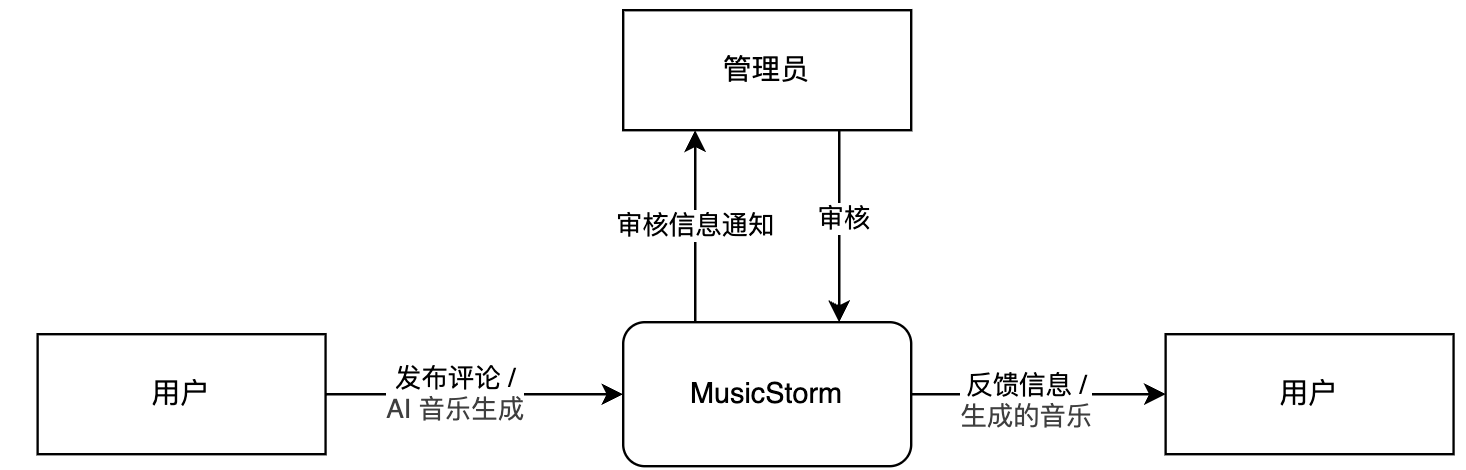
\includegraphics[width=0.8\textwidth]{images/1-1.png}
    \caption{顶层数据流图(上)和一层数据流图(下)}
\end{figure}

\subsubsection{工作负荷}

\textbf{A. 音乐生成模块工作负荷}

系统日均接收音乐生成的多模态输入请求约500次,其中文本输入占比 60\%,平均每次文本输入包含约200字的音乐风格、情绪等描述信息;图像输入占比40\%,日均处理图像文件约200张,每张图像大小在1 - 5MB之间。每次生成请求,预处理模块需对输入数据进行语义分析、特征提取等操作,生成模型需处理约10MB的中间数据来生成初步音乐片段。​

基于 MindSpore 的音乐生成模型,每次生成操作平均需进行100万次以上的浮点运算,以构建音乐的旋律、和声、节奏等元素。在高并发时段(如晚间 7 - 10 点),生成请求量可达平时的 2 - 3 倍,模型需在 10 秒内完成单次生成任务,对服务器的 CPU 和 GPU 计算资源占用率分别达 60\% - 80\% 和 70\% - 90\%。​

\textbf{B. 音乐鉴赏模块工作负荷​}

日均接收音乐鉴赏请求约300次,其中用户上传音乐文件占比30\%,平均文件大小约5MB;社区内其他用户分享音乐的鉴赏请求占比70\%。音频解析模块每次需提取约50项音乐基础特征数据,同时从音乐知识库调取约10MB的标准数据进行比对分析,此外还需处理约1MB的社区用户评价、点赞等交互数据用于综合评估。​

音乐鉴赏分析过程中,每次需进行约50万次的特征比对与数据分析运算,生成鉴赏报告平均耗时3 - 5秒。在热门音乐发布或大型活动期间,鉴赏请求量可能激增50\%以上,对服务器内存和存储I/O性能要求较高,内存占用率达70\%,存储I/O吞吐量需达到50MB/s。​

\textbf{社区交互模块工作负荷}

系统日均处理社区交互操作约2000次,包括作品上传(日均50次,平均文件大小3MB)、评论发布(日均800条,平均每条10字)、点赞收藏(日均600次)、关注操作(日均1500次)等。用户行为数据库每日新增数据量约5GB,其中文本数据占比60\%,文件数据占比30\%,操作日志等其他数据占比10\%。​

社区交互处理模块需实时处理用户操作请求,更新页面展示内容和用户数据。每次交互操作平均需进行1000次以上的数据库读写操作,在用户活跃高峰期,数据库连接数需维持在500以上,对数据库性能要求极高,CPU 使用率达50\% - 70\%,磁盘 I/O 吞吐量需达到30MB/s 。

\subsubsection{费用开支}

模型训练:花费预计1000元,租聘服务器。

后端开发以及服务器搭建:花费预计300元。

\subsubsection{人员}

算法工程师:3人。负责基于 MindSpore 框架开发和优化音乐生成算法、音乐鉴赏分析算法等。

文档指导:2人。项目规划与协作 技术传承与留存 质量把控与版本管理 用户使用与推广

\subsubsection{设备}

笔记本电脑

\subsubsection{局限性}

\textbf{A. 计算性能瓶颈​}

服务器的 CPU、GPU 算力弱,在处理基于 MindSpore 的多模态音乐生成算法,以及复杂音乐鉴赏的音频分析任务时,速度缓慢。多用户同时请求音乐生成,处理时间可达数分钟,难以实现实时响应,严重影响使用体验。​

\textbf{B. 存储能力短板​}

存储设备容量有限,且读写速度慢。随着用户上传音乐、多模态数据及社区交互数据增多,不仅存储空间易饱和,在批量读写音乐文件时,延迟明显,拖慢系统整体运行效率。

\textbf{C. 响应效率低下​}

无法应对稍高的访问量。多人同时测试或模拟少量用户访问,就易出现网络拥堵,导致音乐生成、鉴赏及社区交互功能响应延迟,用户操作反馈迟缓。​

\textbf{D. 功能扩展困难​}

基础硬件配置和简易系统架构,难以支撑新功能开发。增加音乐生成风格、拓展鉴赏维度或丰富社区功能时,现有计算、存储和网络资源无法满足需求,新模型和功能难以部署运行。

\subsection{所建议的系统}

\subsubsection{对所建议系统的说明}

采用微服务架构设计系统,将音乐生成、鉴赏、社区交互等功能拆分为独立的微服务模块,每个模块可独立开发、部署和扩展。基于 MindSpore 的可扩展性,方便接入新的深度学习模型,支持更多音乐生成风格和鉴赏维度的扩展。​

微服务架构遵循单一职责原则和高内聚低耦合原则,将复杂系统拆分为多个小型服务,便于功能的独立维护与扩展。MindSpore 框架的模块化设计与插件机制,为算法和功能的扩展提供了技术支持,使系统能够灵活适应业务需求的变化。

\subsubsection{处理流程和数据流程}

建议系统的处理流程和数据流程在现有系统基础上,优化了分布式计算、微服务模块交互和数据存储架构,提升了处理效率和可扩展性。具体流程如前文所述。

\subsubsection{改进之处}

相对于现存系统,所建议系统在计算性能上通过升级硬件和优化算法,缩短了音乐生成和鉴赏的响应时间;存储能力上采用分布式存储系统,增加了容量和读写速度;响应效率上部署高性能网络设备和负载均衡器,提升了并发处理能力;功能扩展上采用微服务架构,方便新功能的添加和升级。

\subsubsection{影响}

新提出的设备要求包括高性能服务器集群、分布式存储系统、企业级网络设备等,对现存系统中尚可使用的设备需根据实际情况进行升级或替换,以满足新系统的运行需求。

为了使现存的应用软件和支持软件能够同所建议系统相适应,需要对操作系统、数据库管理系统、开发框架等进行升级和优化,同时对现有软件的接口进行调整和适配。

开发团队需掌握 MindSpore 分布式训练、微服务架构设计及音频信号处理技术;运维团队需熟悉企业级服务器集群管理、分布式存储故障排查及网络安全防护策略。

需制定标准化的多模态输入规范(如文本描述格式、图像尺寸要求),并新增音乐版权授权操作流程,确保用户生成内容的合法性。

建立服务器集群监控机制,实时跟踪 CPU/GPU 利用率、存储 I/O 吞吐量等指标,当单节点负载超过 70\% 时自动触发扩容策略。  

采用 “本地磁盘 + 分布式对象存储 + 异地灾备” 三级存储架构,每日凌晨 2 点进行全量数据备份,每小时增量备份,恢复时间目标(RTO)≤30 分钟。

需构建包含 10 万首以上标注音乐的数据集用于模型训练,其中流行古典、电子、风格占比分别为 40\%、30\%、30\%。

开发过程中需对用户音频数据进行脱敏处理,采用AES-256加密算法存储敏感信息,核心代码库实施“双机热备 + 代码评审”机制。

\subsubsection{局限性}

当前基于MindSpore的GAN模型在复杂音乐结构,无法完全模拟人类创作者的灵感迸发过程。图像到音乐的特征转换存在语义偏差。AI 生成音乐的版权归属尚未有明确法律界定,若用户生成内容与现有作品相似度超过80\%,可能引发侵权纠纷。

\subsubsection{技术条件方面的可行性}

MindSpore框架已开源音乐生成预训练模型,经测试在流行音乐生成场景下,可满足基础功能需求。多模态融合技术已在学术领域取得突破,通过迁移学习可适配 MindSpore 框架,当前团队已完成文本 - 音乐映射模块的原型开发。

\subsection{可选择的其他系统方案}

扼要说明曾考虑过的每一种可选择的系统方案,包括需开发的和可从国内国外直接购买的,如果没有供选择的系统方案可考虑,则说明这一点。

\subsubsection{可选择的系统方案 1}

基于 TensorFlow 的音乐生成社区。采用 TensorFlow 框架构建音乐生成模型,结合 Django 搭建社区交互平台,数据库使用 MySQL+Redis 组合。不过 TensorFlow 在分布式训练场景下的通信开销比 MindSpore 高 30\%,无法满足千级用户并发需求。

MindSpore 原生支持华为昇腾芯片,在音频处理任务上的性价比比 TensorFlow+NVIDIA 方案高 40\%。MindSpore 官方提供音乐生成专项技术支持,而 TensorFlow 在音乐领域的案例较少,技术迭代速度较慢。

\subsubsection{可选择的系统方案 2}

租用第三方音乐生成 API(如 Soundful),结合自有社区平台集成,不进行底层算法开发。第三方 API 仅支持基础旋律生成,无法实现多模态输入和参数自定义,不符合项目 “个性化创作” 的核心需求。按调用次数收费,当用户量超过 10 万时,年成本将达 60 万元,远超自建系统的运维成本。用户音频数据需上传至第三方服务器,存在隐私泄露风险,无法满足项目对数据安全的要求。

\subsection{投资及效益分析}

\subsubsection{支出}

在初期投资的第一年,硬件设备的投入主要包括购买十台GPU服务器集群,花费80万元,同时还需购置存储设备和网络设备,分别花费20万元和10万元,合计硬件费用为110万元。在软件开发方面,算法研发的费用为30万元,前端开发20万元,后端开发25万元,以及测试部署费用15万元,软件开发的总费用达到90万元。此外,为了获取版权授权,音乐数据集版权需要支付15万元,而第三方API接口费需要5万元,这两个费用合计为20万元。关于人员成本,研发团队的五名成员年薪总计80万元。其他费用方面,办公场地的租金为10万元,而水电费则为5万元,总计为15万元。因此,第一年的初期总投资为硬件、软件开发、版权授权、人员成本和其他费用之和,即315万元。

进入第二和第三年的运营维护阶段,硬件的持续升级及维护费用每年需要20万元。此外,为了应对不断变化的市场需求,软件开发也需进行功能的迭代及优化,费用每年为30万元。在人员成本方面,研发团队的维护费用每年为60万元。同时,营销推广也是不可或缺的一项支出,每年的预算为40万元。综上所述,第二和第三年的运营维护年投资总额为150万元,这包括了硬件升级、软件开发、人员成本以及营销推广各项费用。

\subsubsection{收益}
在第一年的直接收益方面,会员订阅是重要的收入来源。预计会有10万名注册用户,其中5\%的用户将选择订阅,年费设定为99元,计算得出,会员订阅的收益将达到49.5万元。此外,用户在这一年生成的作品数量预计为5万首,版权交易的抽成比例为10\%,每首作品的平均售价为50元,这样粗略估算版权交易的收益为25万元。与此同时,还计划在第一年与5家企业签约,每家企业的年费为10万元,因此此项的收益将为50万元。综合上述三项收入,第一年的直接收益合计为124.5万元。

到了第三年,预计收益会显著增长。在会员订阅方面,用户数量预计将达到100万,订阅率提升至8\%,这样计算得出会员订阅的收益为792万元。在版权交易方面,预计作品数量将增至50万首,按照每首作品50元的售价计算,版权交易的预计收益为250万元。同样,企业服务方面,预计将签约20家企业,实现的收益将为200万元。此外,还计划通过广告获得100万元的收入。因此,在第三年,直接收益的合计将达到1342万元。

在间接收益方面,提升品牌价值将是这一阶段的重要目标,通过增强企业在AI音乐领域的知名度,为后续产品的研发打下良好的基础。此外,积累的用户行为数据和音乐生成数据将形成一项宝贵的数据资产,这些数据不仅能够进一步优化算法,还将为开拓新业务提供支持。同时,企业的行业影响力也将得到提升,推动AI与音乐产业的深度融合,从而增强在行业内的话语权和影响力。

\subsubsection{收益/投资比}

第 1 年:收益 124.5 万元 / 投资 315 万元≈0.395

第 3 年:收益 1342 万元 /(315+150×2)万元 = 1342/615≈2.18

\subsubsection{投资回收周期}

前 3 年总投资:315+150×2=615 万元

前 3 年总收益:124.5+150×2+1342=124.5+300+1342=1766.5 万元

累计收益超过投资的时间点:第 3 年

具体计算:第 1 年累计收益 124.5 万元,第 2 年累计 124.5+150=274.5 万元,第 3 年到第 3 季度累计 274.5+1342×0.75≈274.5+1006.5=1281 万元 > 615 万元,投资回收周期约 2 年 9 个月

\subsubsection{敏感性分析}


若用户增长速度下降 20\%,第 3 年用户数 80 万,会员收益 792×0.8=633.6 万元,总收益约 1200 万元,收益 / 投资比约 1.95,投资回收周期延长至 3 年 1 个月

若订阅价格下降 10\%,第 3 年会员收益 792×0.9=712.8 万元,总收益约 1262.8 万元,收益 / 投资比约 2.05,投资回收周期约 2 年 10 个月

若运营成本上升 15\%,年运营成本 150×1.15=172.5 万元,前 3 年总投资 315+172.5×2=660 万元,第 3 年总收益约 1342 万元,收益 / 投资比约 2.03,投资回收周期约 2 年 10 个月。

\subsection{社会因素方面的可行性}

\subsubsection{法律方面的可行性}

用户数据存储符合《个人信息保护法》要求,敏感信息加密传输,留存日志不超过 6 个月。

\subsubsection{使用方面的可行性}

该用户适配性设计旨在覆盖多个群体,包括专业创作者、音乐爱好者以及教育机构。其基础功能可以在五分钟内上手,而对于需要使用高级功能的用户,我们也提供了详细的教程支持,以帮助他们充分利用这些功能。在交互体验方面,系统支持多端适配,适合在PC与移动设备上使用,同时保持操作逻辑的一致性。此外,系统能够实时反馈用户的操作进度,并在出现异常情况时能够智能提示,确保用户能顺畅地完成任务。

在社区生态方面,这一平台支持用户进行创作分享、评论互动及主题小组的运营。为鼓励创作,平台设立了创作者排行榜,并开通了版权交易和变现通道,从而激励更多的用户参与创作。在场景验证方面,进行了典型场景的测试,例如图像生成音乐的过程耗时仅为八秒,用户满意度高达4.8/5。调研数据显示,89\%的用户认可多模态功能的实用性,这进一步证明了该系统的价值。

为确保用户顺畅使用,我们提供了完善的支持体系,包括新手引导、帮助中心以及官方技术问答服务。用户还可以在工作日通过在线客服获得 assistance,同时也能查阅API开发文档,以方便开发者进行集成和使用。而在风险应对方面,平台采用“免费 + 订阅”的模式来防止用户流失,并通过智能推荐参数来降低操作的门槛。此外,区块链存证技术的应用有助于保障用户数据隐私,增强体系的安全性与可信赖性。

\subsection{结论}

基于 MindSpore 的架构设计在算法精度和性能上满足需求,团队具备相应开发能力。虽前期投资较大,但在 3-4 年内可实现盈亏平衡,长期收益可观。推动 AI 与音乐产业融合,为创作者提供低成本创作工具,具有良好的社会效益。 
\newpage

\section{系统开发计划}

\subsection{引言}

本计划是我们团队完成“MusicStorm”实践环节的核心指导文件,旨在提高我们教学目标驱动:训练软件开发全流程实践能力以及团队协作意识​,定义软件开发的流程,记录里程碑节点。

\subsection{项目概述}

\subsubsection{工作内容}

\begin{enumerate}
    \item 训练MindSpore模型。
    \item 完成项目App的前端开发
    \item 建立完善的审核机制。
    \item 完成App的后端开发
    \item 整合上述部分,进行整体功能测试以及性能优化
    \item 开源代码,发布正式版本
\end{enumerate}

\subsubsection{主要参加人员}

主要开发人员:孙海洋,夏清伟,胡浩东,陈俊至,于畔湘

孙海洋:主要进行 MindSpore 模型的训练以及后端审核系统
陈俊至,于畔湘:实现项目的前端开发,以及文档编写
夏清伟,胡浩东:实现项目后端主体开发以及软件测试

\subsubsection{产品}

\textbf{A. 程序}

\text{软件 MusicStorm,包含下面文件中展示的 electron 包和 src 包,back\_end 包,front\_end 包、materials 包。这些代码主要实现软件的启动,软件的渲染,软件功能的实现等作用。}

数据库,包括下面文件列表中的datebase包,包中包含了帖子表,帖子-音乐表,用户表,用户-帖子表,用户-帖子-音乐表,音乐表,用户详细信息表。

\textbf{B. 文件}



\textbf{C. 服务}

% Please add the following required packages to your document preamble:
% \usepackage{booktabs}
% \usepackage{longtable}
% Note:It may be necessary to compile the document several times to get a multi-page table to line up properly
\begin{longtable}{@{}llll@{}}
\caption{服务}
\label{tab:my-table}\\
\toprule
\textbf{服务类别} & \textbf{服务内容} & \textbf{开始日期} & \textbf{服务期限} \\* \midrule
\endhead
%
\bottomrule
\endfoot
%
\endlastfoot
%
操作培训服务 & \begin{tabular}[c]{@{}l@{}}1. 管理员培训:后台管理操作\\ 2. 用户培训:音乐生成+鉴赏功能\end{tabular}         & 2025-7-10 & 2025-8-10 \\
技术维护服务 & \begin{tabular}[c]{@{}l@{}}1. Bug修复支持\\ 2. 月度系统健康检查\end{tabular}                    & 2025-7-10 & 2025-8-10 \\
运行支持服务 & \begin{tabular}[c]{@{}l@{}}1. AI生成排队状态查询\\ 2. 版权存证证明导出\\ 3. 分发平台对接状态监控\end{tabular} & 2025-7-10 & 2025-8-10 \\* \bottomrule
\end{longtable}

\textbf{D. 非移交的产品}

% Please add the following required packages to your document preamble:
% \usepackage{booktabs}
% \usepackage{longtable}
% Note:It may be necessary to compile the document several times to get a multi-page table to line up properly
\begin{longtable}{@{}lll@{}}
\caption{非移交的产品}
\label{tab:my-table}\\
\toprule
\textbf{交付项} & \textbf{内容说明} & \textbf{提交期限} \\* \midrule
\endhead
%
源代码仓库        & 含完整Git历史,分支策略 & 答辩当天          \\
AI模型训练资产     & 微调参数集,数据清洗脚本  & 答辩当天          \\* \bottomrule
\end{longtable}

\textbf{E. 验收标准}

% Please add the following required packages to your document preamble:
% \usepackage{booktabs}
% \usepackage{longtable}
% Note:It may be necessary to compile the document several times to get a multi-page table to line up properly
\begin{longtable}{@{}lll@{}}
\caption{验收标准}
\label{tab:my-table}\\
\toprule
\textbf{交付物} & \textbf{验收便准}                                                            & \textbf{验收依据} \\* \midrule
\endhead
%
\bottomrule
\endfoot
%
\endlastfoot
%
决策追踪矩阵       & \begin{tabular}[c]{@{}l@{}}1. 记录≥3次重大技术选型会议纪要\\ 2. 包含备选方案对比\end{tabular} & 会议录像+签字页      \\
每日站会毒瘤记录 & \begin{tabular}[c]{@{}l@{}}1. 标注所有进度延误事件\\ 2. 根本原因分析采用鱼骨图\\ 3. 附改进措施实施证据\end{tabular}                  & 比对甘特图实际进度  \\
代码审查缺陷地图 & \begin{tabular}[c]{@{}l@{}}1. 基于GitLab Merge Request生成\\ 2. 使用热力图可视化BUG分布模块\\ 3. 标注高频问题类别\end{tabular} & 检查原始MR评论记录 \\* \bottomrule
\end{longtable}

\subsubsection{完成项目的最迟期限}

2025年7月9日

\subsubsection{本计划的批准者和批准日期}

2025年6月30日

\subsection{实施计划}

\subsubsection{工作任务的分解与人员分工}

对于项目开发中需要完成的各项工作,从可行性研究、需求分析、设计、实现、测试直到维护,包括文件的编制、审批、打印、分发工作,用户培训工作,软件安装工作等,按层次进行分解,指明每项任务的负责人和参加人员。

% Please add the following required packages to your document preamble:
% \usepackage{booktabs}
% \usepackage{longtable}
% Note:It may be necessary to compile the document several times to get a multi-page table to line up properly
\begin{longtable}{@{}ccccccc@{}}
\caption{MusicStorm项目责任分配矩阵  F:负责  C:参与}
\label{tab:my-table}\\
\toprule
任务/成员           & 可行性研究 & 需求分析 & 概要设计 & 详细设计 & 实现 & 沟通管理 \\* \midrule
\endhead
%
\bottomrule
\endfoot
%
\endlastfoot
%
20222004210孙海洋 & F     & C    & C    & C    & C  & C    \\
20221401231夏清伟 & C     & F    & C    & C    & C  & C    \\
20221401010胡浩东 & C     & C    & F    & C    & C  & C    \\
20221401244陈俊至 & C     & C    & C    & F    & C  & C    \\
20221401235于畔湘 & C     & C    & C    & C    & C  & F    \\* \bottomrule
\end{longtable}

\subsubsection{接口人员}

% Please add the following required packages to your document preamble:
% \usepackage{booktabs}
% \usepackage{longtable}
% Note:It may be necessary to compile the document several times to get a multi-page table to line up properly
\begin{longtable}{@{}lll@{}}
\caption{接口人员}
\label{tab:my-table}\\
\toprule
\textbf{接口方向} & \textbf{负责人} & \textbf{职责范围}                       \\* \midrule
\endhead
%
\bottomrule
\endfoot
%
\endlastfoot
%
用户接口          & 夏清伟          & - 收集用户试用反馈- 管理用户期望                  \\
内部管理接口        &              &                                     \\
财务管理          & 孙海洋          & - 核销设备采购费用 (声卡/服务器)- 审计Suno API调用预算 \\
质量检测          & 胡浩东          & - 监督技术债报告合规性- 抽查代码审计记录              \\* \bottomrule
\end{longtable}

\subsubsection{进度}

\begin{figure}[H]
    \centering
    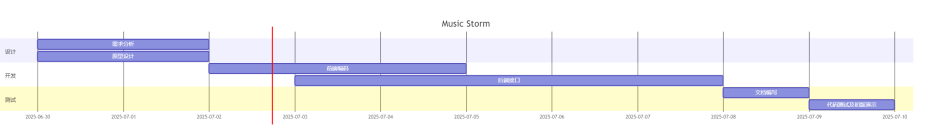
\includegraphics[width=\textwidth]{images/3-1.png}
    \caption{甘特图}
    \label{fig:gantt-chart}
\end{figure}

\subsubsection{预算}

模型训练:孙海洋,花费预计1000元,时间预计4天

前端开发:陈俊至,于畔湘。花费预计0元,时间预计2天

后端开发以及服务器搭建:夏清伟,胡浩东。花费预计300元,时间预计3天

花费来源:自费

\subsubsection{关键问题}

在项目进展方面,我们面临着几个关键的挑战。首先,MindSpore模型的训练尚未完成,这将直接导致AI音乐创作功能无法按计划实现。AI音乐创作是此项目的一个核心亮点,如果不能如期上线,将严重影响用户体验和项目整体吸引力。其次,审核系统目前的完善程度和是否存在漏洞是另一个亟待解决的问题。一个健全且无漏洞的审核系统对于社区的成功搭建至关重要。社区的健康发展必须建立在严格遵守法规、杜绝不良信息传播的基础上。如果审核系统存在缺陷,不仅会影响社区的合法合规性,更可能导致用户流失,阻碍社区的健康成长和发展。因此,我们需要优先解决模型训练和审核系统完善这两个关键问题,以确保项目的顺利推进和社区的成功建立。

\subsection{支持条件}

本项目所需的设备有:

\begin{enumerate}
    \item 能够支持AI训练的服务器设备
    \item 支持存放数据库资料的服务器设备
\end{enumerate}

\subsubsection{计算机系统支持}

开发环境要求:笔记本(5台),测试手机(1台)
软件与工具支持:操作系统(Windows 11),开发工具(Android stdio +VScode+Gitlab),AI模型(MindSpore),数据库(MySql)
云服务器:华为云(8核16G)

\subsubsection{需由用户承担的工作}

% Please add the following required packages to your document preamble:
% \usepackage{booktabs}
% \usepackage{longtable}
% Note:It may be necessary to compile the document several times to get a multi-page table to line up properly
\begin{longtable}{@{}llll@{}}
\caption{需由用户承担的工作}
\label{tab:my-table}\\
\toprule
\textbf{工作模块} & \textbf{具体任务} & \textbf{负责人} & \textbf{完成期限} \\* \midrule
\endhead
%
\bottomrule
\endfoot
%
\endlastfoot
%
需求分析          & 用户需求模拟        & 陈俊至          & 6月30日         \\
              & 需求分析优先级排序     & 全体           & 6月30日         \\
环境搭建          & 开发设备配置        & 全体           & 7月1日          \\
              & 本地Gitlab配置    & 全体           & 7月1日          \\
数据准备          & AI训练          & 孙海洋          & 7月4日          \\
              & 音乐数据采集        & 于畔泪          & 7月2日          \\
项目开发          & 完成前端开发        & 陈俊至, 于畔泪     & 7月4日          \\
              & 完成后端开发        & 夏清伟, 胡浩东     & 7月7日          \\
              & 完成信息审核系统      & 孙海洋          & 7月7日          \\
测试准备          & 虚拟测试用户创建      & 全体           & 7月8日          \\* \bottomrule
\end{longtable}

\subsubsection{由外单位提供的条件}

无

\subsubsection{计算机系统支持}

无

\subsection{专题计划要点}

无
\newpage

\section{系统(软件)需求规格说明}

\subsection{引言}

软件需求规格说明书(SRS)在项目管理中扮演着至关重要的角色,主要体现在以下四个方面。首先,它有助于定义项目范围并达成共识。通过明确系统功能的边界,例如明确Music Storm仅支持AI生成音乐而不支持乐谱编辑,SRS能够有效解决“我们要做什么”这个根本性问题,从而避免在开发过程中出现需求蔓延(Scope Creep)的情况。这份文档作为项目组、导师和评审委员会共同认可的基准契约,一旦签字,便具有约束力。

其次,SRS为项目的设计与开发提供了明确的指导。设计人员可以依据SRS中对功能的详细描述(例如“支持哼唱输入生成音乐”),来选择合适的技术路径,比如采用音频FFT转换Mel频谱的技术。同时,SRS也为开发任务的分解提供了依据,使得需求项能够被细化为具体的JIRA任务,例如“MUSIC-102:实现哼唱转MIDI接口”等。

再者,SRS是质量控制和验收标准的重要来源。每一条需求都应能够直接映射到相应的测试用例,比如需求ID REQ-205对应测试用例TC-205,用于验证10秒哼唱是否能生成30秒音乐。在项目验收阶段,答辩评委也将依据SRS逐条核对功能的实现情况,确保项目交付物符合预期。

最后,SRS在风险管理和变更控制中发挥着关键作用。通过早期识别并暴露不可行的需求(例如“实时生成交响乐”因算力限制而无法实现),项目团队可以及时进行调整。此外,任何对需求的修改都需要以SRS为基准,评估其对关联模块可能产生的影响,例如修改版权存证流程可能会对分发模块造成影响,从而实现有效的变更控制。

\subsection{任务概述}
\subsubsection{目标}

该项目的开发意图、应用目标、产品描述、产品功能及安全性方面均有详细规划。

在开发意图上,项目主要受到教学价值的驱动,旨在通过全栈开发(包括AI集成、区块链版权保护和跨平台部署)来培养学生解决复杂工程问题的能力,并促进《人工智能》、《软件工程》和《知识产权法》等课程知识与实际项目的融合。同时,项目也致力于技术创新验证,探索生成式AI在艺术创作领域的应用边界,并构建去中心化版权管理的最小可行模型。此外,项目还希望赋能校园场景,通过降低音乐创作门槛,让非专业学生也能利用文字或哼唱创作个性化作品,并建立创作与分享的闭环,从而激发校园艺术创作氛围。

在应用目标方面,项目旨在实现跨学科能力的融合,整合计算机科学(AI模型集成)、音乐学(和声规则分析)和法学(数字版权协议)等领域的知识。项目还致力于完成工程实践的闭环,让学生经历软件开发生命周期的全流程实践(从需求分析到部署运维),以培养工业化工程思维。同时,项目的一个重要目标是教学资产的沉淀,提炼出可复用模块(如音频指纹算法实验包),并将其纳入学校的《创新实践》课程资源库。

产品描述方面,Music Storm被定位为一款面向高校场景的AI驱动音乐创作与鉴赏社区平台。它通过降低创作门槛(支持文本或哼唱生成音乐)、构建版权保护闭环(区块链存证)以及提供沉浸式社区互动,旨在激发校园艺术创作生态。

产品功能上,Music Storm的核心功能围绕创作、保护和分享展开。AI创作引擎提供便捷的音乐生成能力,用户可以输入文本描述(如风格、情绪)在30秒内生成具备专业编曲水平的音乐片段,涵盖流行、电子、古典等10种常用风格。用户也可以通过哼唱约10秒的旋律,AI智能识别并补全发展为结构完整的乐曲,并支持将生成的音乐导出为标准MIDI文件以便二次编辑。版权管家功能则保障创作成果,作品生成瞬间通过校内区块链节点“一键存证”,生成含精准时间戳和作品数字指纹的电子版权证书。此外,系统还运用先进的音频指纹比对技术,提供24小时全网“侵权追踪”服务,发现侵权时自动发起合规下架请求。鉴赏社区功能搭建了展示与互动平台,独特的“动态乐谱”功能会随音乐播放同步呈现滚动的乐谱视图,用户可自由开关不同乐器声部以深入理解编曲细节。平台还建立了结构化的“挑战赛体系”,允许社团等组织发起特定创作主题,鼓励用户提交AI生成作品参与竞争,优胜者不仅获得社区认可,还能赢得校内线下演出资源扶持。这三大功能共同构成了支持用户从创作、确权到展示推广的全流程服务闭环。

在安全性方面,该系统采用了综合的加密技术和严格的管理策略来保障用户数据安全。用户的登录凭证通过哈希加密算法进行高强度加密,并配置128位长度的盐值以增强安全性。所有上传的音频文件在存储环节均通过国家商用密码标准的SM4算法加密,其加解密密钥由学校网络中心统一管理。系统的数据处理遵循“全生命周期管控”原则,核心是数据最小化和流程安全。在数据采集源头,严格实施最小化原则,仅收集必要的OpenID、昵称和头像等基本识别信息,明确禁止获取学号、手机号等个人敏感信息。数据传输全程强制使用HTTPS协议,并应用SSL Pinning技术,有效防范中间人攻击风险,确保数据在传输过程中的完整性与机密性。隐私合规设计体现在精细的数据使用授权和脱敏处理上。系统建立了分级授权机制,用户分享作品时需独立勾选具体的授权范围选项。对于用于训练和优化AI模型的数据,系统会对收集到的作品进行严格脱敏处理,确保去除任何可关联到创作者个人身份的信息,仅保留作品的非识别性特征标签,在促进技术发展的同时充分尊重并保护用户的个人隐私权益。

\subsection{软件的一般性描述}
\subsubsection{软件产品与其环境之间的关系}

系统的运行高度依赖特定的硬件设施并与之紧密互动。关键计算任务——特别是在本地执行的 AI 推理(如 MusicGen 模型)——依赖于实验室专用的 GPU 服务器,其使用受到时段限制,生成任务需要预约每周三和周五下午的设备开放时间才能进行。专业音频输入环节则需调用数字媒体教室配置的专业设备(如罗德麦克风和 Focusrite 声卡)进行哼唱录制,设备的管理受学校《仪器管理条例》约束,损坏需按规追责。为应对设备非开放时段的需求,系统配置了适配策略:自动启用云端弹性算力进行任务分流。同时,部署的设备健康监测模块将持续追踪关键音频设备的使用时长,一旦声卡累计工作时间超过 500 小时,将自动停用该设备并触发报修流程。

​​在软件层面,系统通过内外部集成实现核心功能与流程。内部集成方面,系统通过 OAuth2.0 协议与教务管理系统连接,同步用户的课程表数据,并据此在考试周等特定时段自动进入低功耗静默模式以减少干扰。身份认证环节则通过集成学校的 LDAP 系统实现统一认证,学生使用学号及密码登录,教师用户在该体系中自然获得优先审核等权限。外部服务耦合则涉及两个核心组件:AI 音乐生成主要依赖公网的 Suno API 服务,但由于校园网策略限制其国际访问,所有对 Suno API 的调用必须经过部署在境内的代理服务器进行中转;版权存证功能则通过对接设在校内的“新版链教育节点”(一个私有区块链)实现,系统会将作品的哈希值写入该区块链,同时将存证信息同步记录至教务系统内的课程作品库,以作校内追踪。

​​系统建立了预设的异常处理流程以保障核心服务的连续性。当检测到对 Suno API 的请求因调用频率过高而被限制(超频)时,系统会立即触发自动降级机制,切换到本地部署的 MusicGen 模型继续提供服务,此切换需保证用户感知到的延迟不超过 120 秒。若对接的校内私有链节点出现异常导致版权存证写入失败,系统会执行应急方案:将待存证的数据暂时转存至预置的 MySQL 应急数据库,并同时触发邮件告警通知管理员进行人工干预,确保业务中断期间数据不丢失并可后续追补。

\subsubsection{限制与约束}

系统在功能设计上设定了明确的边界限制。在创作范围方面,AI音乐生成功能支持包括流行、电子、古典在内的10种基础音乐风格,但明确不支持交响乐或实验音乐等需要复杂编曲的类型;单次生成音乐片段的时长上限为90秒,系统不提供完整乐曲的创作能力;在人声合成领域,仅能实现简单的合唱或说唱片段生成,不具备模拟特定歌手(如周杰伦式)独特音色的能力。版权管理服务同样存在限定,其区块链存证服务目前仅覆盖中国大陆地区,无法处理境外版权登记请求;同时该服务仅登记数字音乐作品本身版权,不涉及影视配乐授权或商业音乐授权等更为复杂的场景。社区互动功能也有其约束:平台采用AI实时过滤加管理员审核的双重机制进行内容监管,虽然部署了敏感词库拦截,但仍存在方言谐音梗漏检的可能性;社交功能上,仅提供基础的点赞和评论能力,不包含私信或群聊功能。

性能方面设定了严格的效率上限与资源容量阈值。生成速度受到制约:基于文本描述生成音乐的请求,要求在95\%的情况下响应延迟不超过5秒;而依靠哼唱输入生成音乐的请求,则受频谱转换处理速度影响,目标延迟控制在8秒以内。系统的高并发能力也存在瓶颈,在标配(2核CPU/4GB内存)的单台服务器环境下,其最高承载能力为200名同时在线并执行核心操作的用户,超出此负载将向用户返回系统繁忙提示。资源容量限制体现在存储和计算两个层面:用户的免费存储空间配额为5GB(基于NAS存储),超出后需向教师提交扩容申请进行人工审批;每日AI音乐生成任务总量受限,受限于Suno API的配额及本地GPU服务器算力,其硬性上限设定为800次/日。

技术实现层面存在关键的环境与集成约束。开发环境强制规定:后端服务必须使用Java语言并基于Spring Boot框架实现,而前端界面则必须确保与过时的IE11浏览器完全兼容(以满足教务系统访问要求)。对于项目依赖的第三方组件,存在严格的许可限制:禁止使用任何要求公开源代码的组件(如GPL协议的库),仅允许集成采用Apache或MIT这类宽松许可证的库。在系统集成方面,数据互通能力被严格限制,仅被允许单向从指定的外部系统(教务系统、图书馆管理系统)读取特定数据,例如读取用户课程表数据以自动设置静默免打扰模式,禁止向这些系统写入数据。

\subsubsection{假设与前提条件}

开发阶段的推进基于一系列关键前提条件。​​ 首先是对算力资源的假设:项目计划持续使用华为云 ModelArts 提供的教育配额(每月约1,000元人民币额度)以及 Suno API 教育版的免费调用限额(每月5,000次)。如果突破这些限额,项目将需要额外自筹资金,预计每月至少3,000元人民币用于补充云资源,否则将不得不启动降级预案,切换到本地部署的 MusicGen 模型来维持基本功能。其次,技术框架的稳定性被高度依赖,核心假设是选用的 Spring Boot 3.x、React Native 0.70 等主要技术框架在其项目开发周期内不会发生带有破坏性的重大更新。倘若发生颠覆性升级,项目团队需重新评估迁移成本,预计这可能导致项目交付延期最多两周时间。再者,跨部门协作的通畅性至关重要,假设法学院(负责版权条款审核)、设备管理处(负责硬件维修)以及信息中心(负责网络等基础设施)等校内相关部门对于协作请求的响应时效应控制在48小时以内。如果出现协作延迟,项目将通过校内加急流程机制进行缓解,目标是将关键路径上的延期影响控制在15\%以内。最后,项目的合规运作依赖于法律法规环境的稳定,当前假设《生成式AI服务管理暂行办法》第12条(关于免责的条款)在2025年前不会发生影响项目合规性的修订。倘若该法规发生变更,项目需依赖法学院在72小时内出具应急解读报告及修订建议指导。

​​运行阶段的系统功能发挥依赖于多个用户与环境前提。​​ 在用户层面,基本设定是学生创作者具备基础的乐理概念(如节奏、风格等),能够相对清晰地描述其音乐创作需求;同时,乐观预测至少有60\%的用户是出于个人兴趣或课程作业的实际需求而主动使用系统进行创作,而非被强制使用。在校园基础设施层面,系统有效运转的前提是校园内网的平均网络延迟不超过200毫秒且丢包率低于1\%;支撑AI计算的本地硬件设施(如实验室的GPU服务器)的年故障率预期不超过5\%,并且假设设备管理处能够确保充足的备件库存以应对故障。关于数据供给的质量,核心假设之一是用于模型训练的外部开放音乐素材库(如 FreeSound CC0 库)将持续可用,且其内容合规率需保持在99\%以上;另一个重要前提是用户使用手机麦克风输入的哼唱录音质量达到基础标准,即信噪比(SNR)不低于20分贝。

​​系统运行还面临着无法完全控制的诸多外部前提约束。​​ 对第三方服务的依赖伴随着风险:Suno API 的服务可用性被假设为不低于99.9\%,如果其可用性降低至95\%以下,项目计划启动本地化的替代方案进行应对;同时,系统依赖的区块链教育节点(版权存证用)的安全性建立在该节点无重大安全漏洞的假设之上,这需要依托区块链实验室出具的年度审计报告来验证。在版权法律环境方面,项目预设司法机关对区块链存证的采信率能够维持在不低于90\%(参照2023年的行业基准值),并且默认由系统生成的用户原创内容归属清晰无争议,即作品生成者被认定为原始著作权人。在用户行为边界层面,一个基本的、但项目团队无法直接确保的前提是“学生不作恶”——即用户不会故意利用系统生成涉及暴力、歧视等违禁内容,也不会发起恶意的版权诬告行为。

\subsection{软件功能需求描述}

\subsubsection{软件功能概述}

该项目的核心创作功能聚焦于AI音乐生成与版权保护。关键功能是通过AI技术,允许用户输入文本描述或录制哼唱,在30秒内快速生成一段60秒的原创音乐片段。这项功能的最高优先级(P0)被认定为核心产品价值,主要服务于学生制作班会视频配乐或社团招新宣传曲等校园常用场景。与之紧密关联的是版权一键存证服务,作品生成后将自动为其创建包含时间戳和创作者身份信息的区块链版权证书,并支持PDF格式下载,同样标为P0优先级。此功能旨在有效保护学生的课程设计等作品版权,避免潜在的抄袭争议。

社区互动功能旨在提升专业性与参与感。其中一项重要功能是动态乐谱播放,在用户收听作品时同步显示可滚动的乐谱,并可选择性地开关不同乐器声部(例如钢琴、鼓组等)。作为P1优先级的功能,它提升了产品的专业度,适用于音乐课堂上分析AI作品的结构,帮助学生理解编曲逻辑。另一项P1优先级的社区功能是主题挑战赛,社团等组织可以发布特定创作主题(如“毕业季”),用户可以提交其AI创作的作品参与,并进行投票评选出前十名。这一功能在校园艺术节预热等活动中能有效激发学生群体的创作热情。

针对校园特定场景,还规划了一套工具箱功能。情绪音乐墙被标记为P2优先级,作为场景增值服务,它部署在图书馆等公共场所的终端设备上,用户输入心情关键词(例如“专注”或“放松”)即可生成适配的环境背景音进行循环播放,服务于自习室氛围调节、缓解考试焦虑等实际需求。同样属于P2优先级的毕设支持中心功能,则专为艺术类专业学生打造,提供免版权的配乐库资源,并支持通过API调用来生成专属的背景音乐(BGM),目的是帮助数字媒体等专业的学生在毕业设计中,用原创或免费配乐替代需要采购的商业音乐。

\subsubsection{软件需求的用例模型}

% Please add the following required packages to your document preamble:
% \usepackage{booktabs}
% \usepackage{longtable}
% Note:It may be necessary to compile the document several times to get a multi-page table to line up properly
\begin{longtable}{@{}ll@{}}
\caption{用例模型}
\label{tab:my-table}\\
\toprule
\multicolumn{1}{c}{\textbf{属性}}                                        & \multicolumn{1}{c}{\textbf{描述}}                                                   \\* \midrule
\endhead
%
\bottomrule
\endfoot
%
\endlastfoot
%
用例名称            & 发布音乐       \\
参与角色            & 创作者        \\
目的                                                                     & 将AI生成的音乐作品发布到社区,完成版权认证并上线                                                         \\
触发条件            & 用户将音乐作品并发布 \\
前置条件                                                                   & \begin{tabular}[c]{@{}l@{}}1. 用户已登录并通过系统认证\\ 2. AI音乐生成已完成并保存到"我的作品"库\end{tabular} \\
后置条件            & 管理员审核音乐    \\
参与者动作           & 系统响应       \\
\begin{tabular}[c]{@{}l@{}}1. 创作者选择"我的作品"\\ 中待发布的音乐显示作品预览\end{tabular} &                                                                                   \\
2. 输入作品信息:      &            \\
- 标题(≦ 30字)     &            \\
- 风格标签          &            \\
- 创作灵感描述        &            \\
3. 设定可见范围       &            \\
4. 选择“同意版权协议”   &            \\
5. 选择“同意版权转载协议” &            \\
                & 执行版权区块维护认证 \\* \bottomrule
\end{longtable}

\subsubsection{软件需求的分析模型}

\begin{figure}[H]
    \centering
    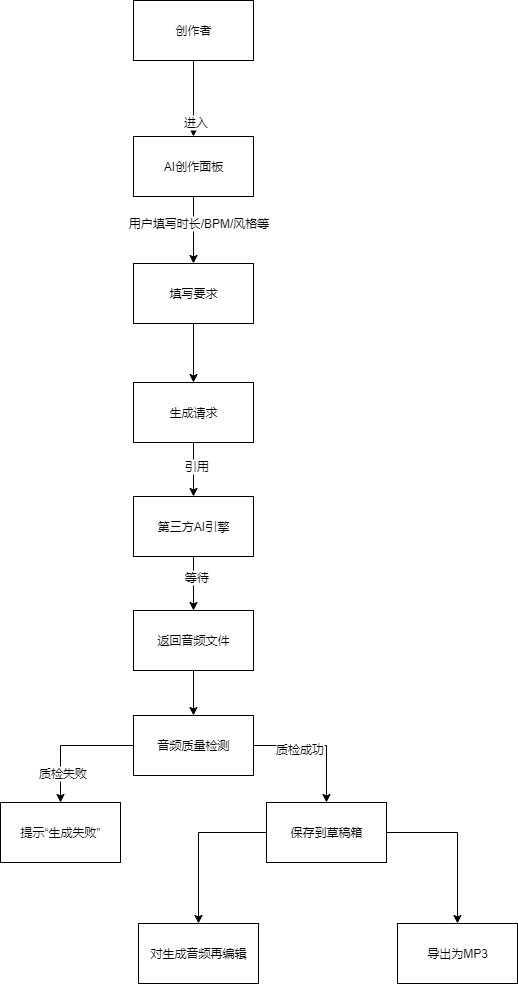
\includegraphics[width=0.7\textwidth]{images/4-1.png}
    \caption{分析模型}
\end{figure}
\begin{figure}[H]
    \centering
    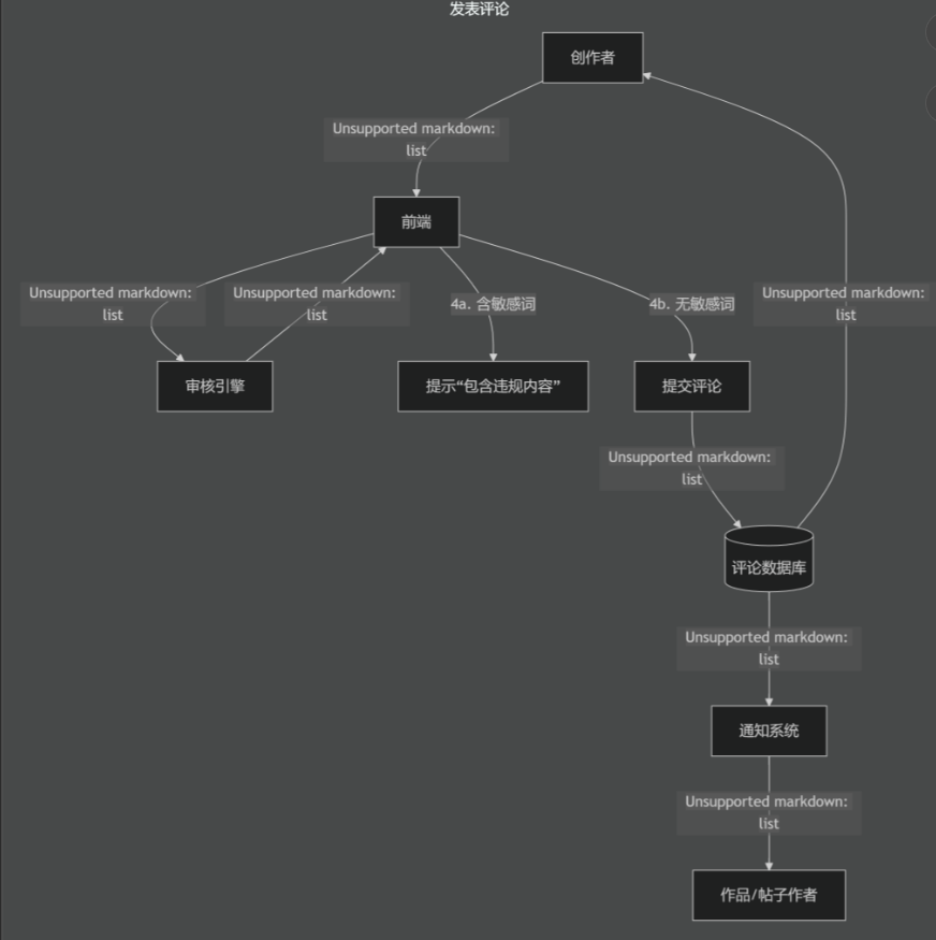
\includegraphics[width=0.7\textwidth]{images/4-2.png}
    \caption{分析模型}
\end{figure}
\begin{figure}[H]
    \centering
    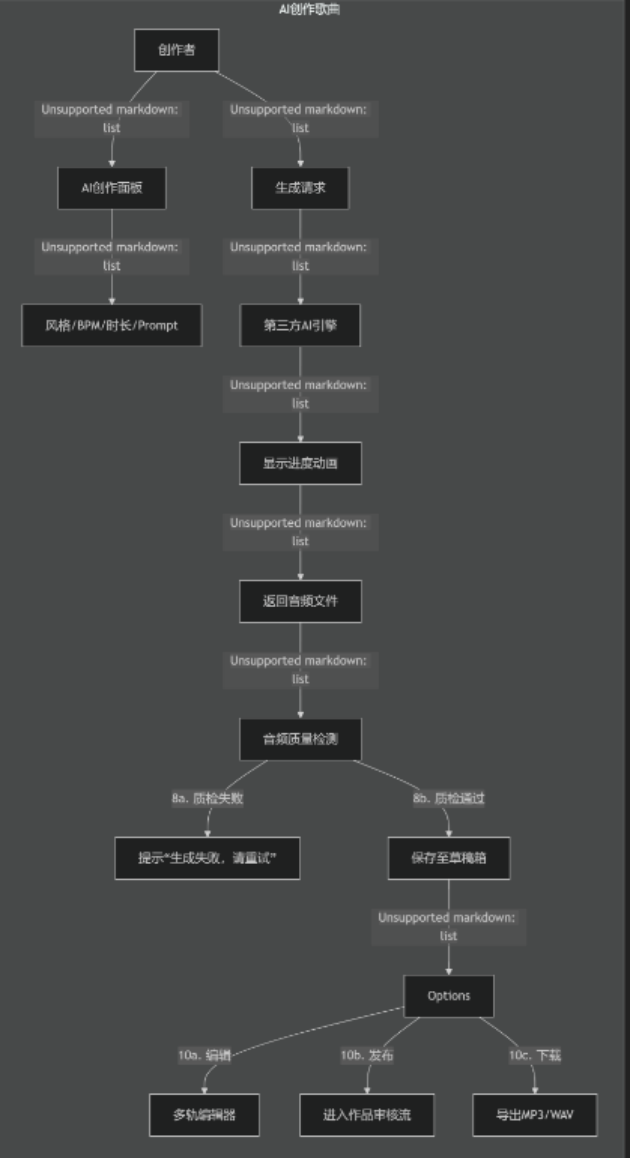
\includegraphics[width=0.6\textwidth]{images/4-3.png}
    \caption{分析模型}
\end{figure}

\subsection{其它软件需求描述}
\subsubsection{性能要求}

系统性能的核心要求体现在响应速度上。普通页面(如用户主页、作品列表页和社区动态页)的首屏内容加载时间必须保证90\%以上的用户在2秒内完成加载。对于包含音频预览或播放器的复杂页面,其首次加载允许在3秒内完成,但后续的播放、暂停等用户交互操作的响应必须控制在0.5秒以内。用户操作的直接反馈也有严格要求:按钮点击操作(例如发布、评论或点赞)的响应延迟不应超过1秒;涉及数据处理的操作(如作品文件上传或设置AI生成参数)的提交确认反馈应在1.5秒内返回。针对AI音乐生成功能,30秒以内的短片段生成平均时间需在20秒内完成,并且在界面上实时显示生成进度;超过30秒的长片段则设定3分钟为生成时间上限,此类任务将转为异步处理机制处理,并在完成后通过电子邮件或站内消息通知用户。

系统需具备强大的吞吐量和并发处理能力,确保可支撑超过1000名用户同时在线,并能有效处理至少200名并发用户进行的核心操作(如作品上传、启动AI生成、发表评论等)。在关键操作容量上,系统必须支持50条以上的并发作品上传任务(假设平均文件大小不超过50MB),AI生成请求队列需有能力应对每分钟超过100个请求的峰值压力,同时后台审核系统应达到管理员每分钟并行审核超过10个作品的效率。

资源利用率方面规定了明确的约束边界。在服务器资源使用上,CPU的平均利用率须控制在70\%以内,内存占用率亦不得超过80\%。在网络传输方面,需要实施优化措施,特别是针对音频流媒体的带宽占用,应采用自适应码率技术;图片资源的加载则必须使用WebP格式并结合CDN缓存策略,确保为原始流量节省40\%或以上。

稳定性与可用性目标定义了系统可靠性的基准。系统的核心服务(作品上传、音频播放、社区功能)全年整体可用性指标要求达到99.5\%或更高。同时,AI生成服务必须具备独立的降级机制设计(如发生故障时自动关闭以保护其他功能正常运行)。在故障恢复方面,系统需确保非灾难性的服务故障能够在5分钟内完成自动恢复过程;对于因故中断的用户操作(例如上传流程),系统必须实现草稿内容的自动保存,并能够恢复至少90\%的已操作内容。

数据处理能力覆盖了文件处理和数据库操作。文件处理方面,要求音频文件从MP3格式转码为AAC格式的平均处理时长不超过原始音频文件时长的30\%(需应用硬件加速技术),单张封面图片从3000像素压缩到800像素的耗时应控制在2秒之内。数据库操作需要维持高性能:复杂查询的响应时间应保证在1秒以内完成返回结果,而数据库写操作(如数据插入、更新、删除)的延迟应始终低于500毫秒。

\subsubsection{设计约束}

开发环境的构建需严格遵循特定的技术要求。后端服务的开发强制要求使用 Java 语言,并基于 Spring Boot 框架进行实现。在用户端方面,前端代码必须确保与较旧的 IE11 浏览器完全兼容,这是一个硬性规定,以满足教务系统用户的访问需求。对于项目依赖的第三方组件,存在明确的许可限制政策:严格禁止引入任何许可证要求公开源代码的组件(例如采用 GPL 协议的库),只允许集成和使用基于 Apache 或 MIT 这类宽松许可证的开源库。

在系统集成层面,主要的约束体现在与外部系统(特别是教务系统和图书馆管理系统)的数据互通方式上。系统仅被允许以单向、只读的方式访问这些外部系统的特定数据接口,即仅能从中读取信息,而严禁向这些系统写入数据。一个具体的应用场景是读取用户课程表数据,用于在相关课程时段内自动触发音乐应用的静默免打扰模式,确保功能实现的同时遵守数据接口的调用限制。

\subsubsection{界面要求}

设计遵循几个核心原则以确保产品的质量和用户体验。首先,严格保持用户界面与 Material Design 3.0 规范的一致性,并采用响应式布局以适应不同设备屏幕尺寸。其次,通过运用暗色调为主的配色方案并结合动态的声波视觉元素,力求营造浓厚的音乐沉浸感。最后,为创作者用户提供便捷体验,支持常用操作的键盘快捷键,并保证核心功能操作流程能在三步或更少的步骤内完成。

在产品的主体核心页面上,左侧区域设计有固定的导航侧边栏,其包含指向仪表盘、作品管理、社区动态和系统通知等主要功能模块的入口。页面的中央核心位置被规划为创作区,该区域集成了完整的作品上传功能(支持文件拖拽并配有元数据信息录入表单)、用于选择创作风格的可视化卡片、用于输入引导生成详细描述的 Prompt 输入框以及调整相关参数的滑块控件,并设置了一个明确的“生成”触发按钮。而页面的右侧则设置为预览区,用于实时展示生成音频的波形图并提供播放控制组件供用户试听。

社区被命名为“社区广场”并单独设计页面,其内容展示采用高效的双列瀑布流布局。在此布局中,创作者发布的动态信息以及包含音乐作品的卡片得以清晰呈现,每条内容都配有评论、点赞等互动功能组件。广场特别提供了两个关键功能:一个是一键“Remix”选项,允许用户基于其他创作者的作品快速发起新的AI再创作;另一个则是深度讨论区,使用话题标签页的方式来组织围绕特定主题的深入交流。

面向管理员设计的审核后台界面则强调效率与批量处理能力。系统内置标签分类器(主要用于识别并分类处理如版权风险、音质过差、内容违规等问题),同时提供高度便捷的批量操作支持。后台配备了清晰标注的快捷批复按钮(“通过”、“拒绝”、“需要修改”),管理员可以基于分类结果快速对多条待审内容进行批量操作决策,大幅提升审核工作效率。

\subsubsection{进度要求}

从6月30日正式启动项目并完成需求分析开始。
进入7月后,开发工作按日推进:7月1日的目标集中在基础设施方面,要求完成数据库建模、API设计以及用户系统的构建;7月2日的重点转向创作者后台,需搭建其基本框架并实现作品上传存储功能;7月3日则是核心功能开发日,需交付AI生成模块的原型版本和一个基础音频播放器。

随后两天的任务围绕审核与社区进行:7月4日需要建立审核后台的框架并实现作品审核的状态机逻辑;7月5日的工作是上线社区动态发布功能、评论系统以及相关的通知机制。

项目后期聚焦于工具完善和系统优化:7月6日的交付物包括用于提升审核效率的审核批处理工具和保障社区内容的敏感词过滤系统;7月7日将进行全面的端到端流程验证,并对系统整体性能进行优化打磨。

\subsubsection{交付要求}
可运行的系统将提供为 Docker 镜像格式,镜像是名为 musicstorm/prod:v1.0.0 的完整微服务容器包,其中封装了 Web 前端(基于 React 框架)、后端 API 服务(使用 Node.js 构建)、AI 集成适配层(采用 Python 开发)以及必要的数据库初始化脚本。

为了满足本地测试环境的部署需求,系统同时提供独立部署包,它是一个 VMware OVA 格式的虚拟机模板,可以直接导入使用。

系统的源代码资产将以代码仓库的快照形式提供,文件命名为 musicstorm-src-20250709.zip。这个压缩包包含了使用 React 结合 Redux 状态管理开发的完整前端工程及其单元测试,基于 Node.js 实现的微服务后端(其 API 文档由 Swagger 工具自动生成),以及用于 AI 系统集成的 Python 适配层代码。所有源代码均附带一个名为 LICENSE.md 的开源协议声明文件,其中详细注明了项目依赖的第三方库及其许可信息。

数据库相关资产主要包括 PostgreSQL 数据库的表结构定义文件 schema.sql,该文件内含有对索引优化的注释说明,以及用于系统初始化的关键数据,如审核规则库和音乐标签分类表的 CSV 格式数据文件。

\subsubsection{验收要求}

核心创作流程确保创作者能够顺利完成从上传作品、AI生成处理到提交审核并查看状态的全部步骤,要求该完整流程的成功率不低于95\%,该结论基于10组样本的测试验证结果;同时明确规定了必现Bug的判定标准,即在流程中出现元数据丢失、文件损坏或流程中断任意一种情况,均视为该流程未成功通过。

审核管理部分要求管理员具备高效处理能力,需在1分钟内完成对5条待审作品的处理操作,处理内容包含播放音频片段及完整填写驳回原因;一旦作品被驳回,系统必须确保相应的驳回信息在10秒内实时推送至创作者的平台通知中心。

社区交互功能重点关注响应速度和内容安全。在模拟千人同时在线的压力测试场景下,用户发布动态或评论的响应时间必须控制在1秒之内;系统配备的敏感词过滤机制要求具有高准确性,使用包含500多个违规词的专用词库进行验证时,其拦截准确率需达到90\%以上(或表述为漏报率不超过10\%)。

AI系统对其生成效率及质量有严格要求。该系统的音频生成任务,对于一段30秒的音频生成请求,其处理耗时不能超过25秒,且在连续发出10次请求的场景下,满足此耗时的达标率需为100\%;在生成音频的质量方面,通过专业的音频分析软件(如FFT)检测,必须确保生成结果无任何音频断裂或爆音现象,检测到的信号信噪比(SNR)需大于或等于30分贝。s

\subsection{软件原型}

\begin{figure}[H]
    \centering
    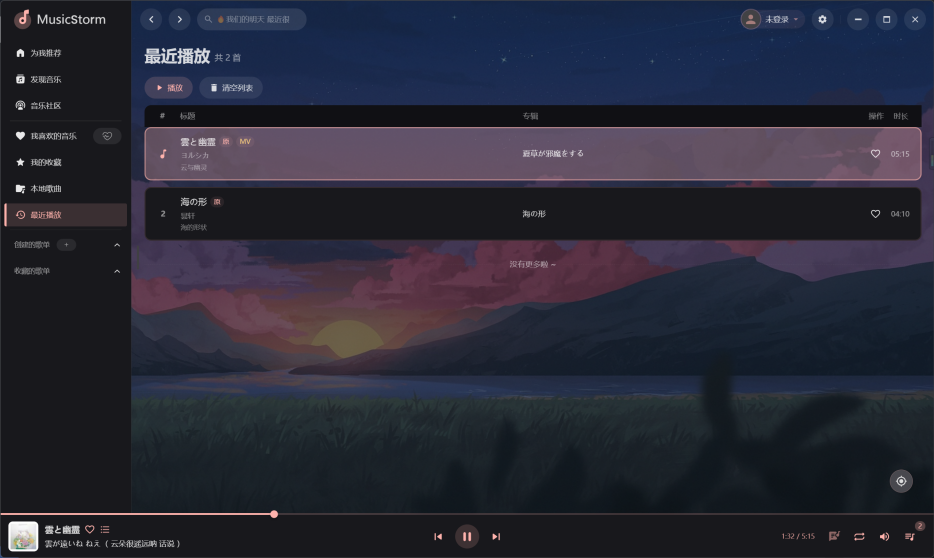
\includegraphics[width=\textwidth]{images/4-4-origin.png}
    \caption{音乐社区}
\end{figure}

MusicStorm提供了一系列核心功能来满足用户的听歌、探索和交流需求。“为我推荐”功能通过分析用户的个人偏好,专门生成个性化的歌单和歌曲推荐。“发现音乐”则是用户探索广阔音乐世界的入口,可以在此浏览新歌、热门榜单以及按不同类别归类的音乐内容。

应用内设有一个专门的“音乐社区”区域,作为用户互动交流的平台,支持音乐分享、发表评论以及其他社交功能。“最近播放”功能会自动记录并展示用户近期听过的歌曲列表,方便快速找回。“我喜欢的音乐”等同于用户的收藏夹,点击即可集中查看所有特别标记为喜爱的歌曲。

对于歌单管理,用户可以通过“创建的歌单”功能入口来制作并管理自己定制的歌单列表。而“收藏的歌单”则服务于保存和便捷访问其他用户创建、您感兴趣并保存下来的歌单内容。整体功能架构清晰,致力于提供全面且便捷的音乐体验。

\begin{figure}[H]
    \centering
    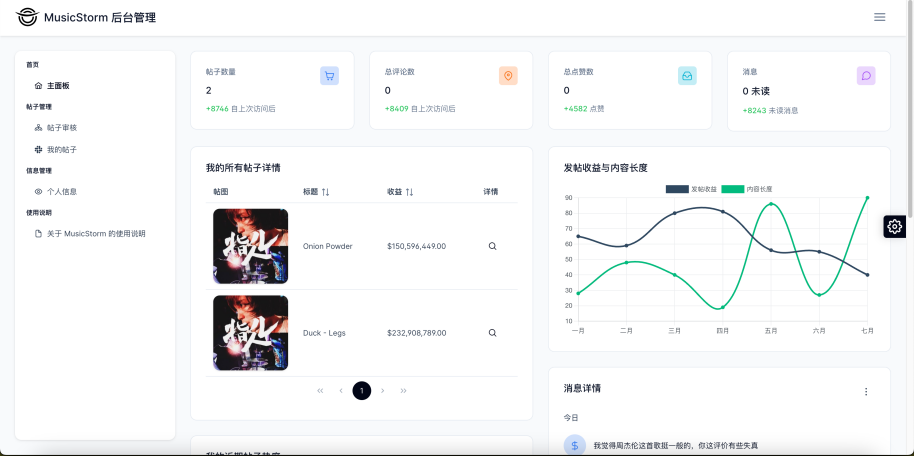
\includegraphics[width=\textwidth]{images/4-5.png}
    \caption{音乐社区后台审核}
\end{figure}

MusicStorm 的后台管理界面为管理员提供了一个清晰、高效的集中管控平台。整个界面采用简洁的灰白配色,布局分明。左侧设置了核心的功能导航栏,包含指向各个管理模块的入口:管理员可以通过“首页”返回主视图,“主面板”可能是核心数据仪表盘,“帖子管理”及细分出的“帖子审核”用于内容管理,“我的帖子”允许管理员查看自己发布的公告或内容状态,“信息管理”及其下的“个人信息”和“使用说明”则涵盖了账户设置和平台操作指南。

界面的主体区域集中在右侧,是综合的数据展示与操作区。最上方区域设计为关键数据概览卡片,直观地显示全局统计数据及其动态变化:包括当前总“帖子数量”以及自上次访问后显著增加的新帖、总评论数、总点赞数;以及系统消息状态这些增量数据是监控平台活跃度和内容增长的核心指标。

紧接着下方是“我的所有帖子详情”区,此处以表格形式详细列出了管理员关联帖子的信息,包含帖子的预览图(帖图)、名称(标题)和产生的收益(收益)。每个帖子条目旁应提供操作按钮(如“详情”)以进行管理。

​​右侧区域则主要用于可视化分析​​,展示了一个名为“发帖收益与内容长度”的图表(类型可能是折线图或柱状图,示例时间为“今日”),该图表旨在分析发布内容的长度(如文字或视频时长)与其所带来收益之间的关联趋势,为内容策略优化提供依据。

​​最底部设有“消息详情”区​​,用于展示具体的信息内容片段,例如图中示例显示了一条用户的评论:“我觉得周杰伦这首歌挺一般的,你这评价有些失真”。这一区域便于管理员快速查看和响应具体的用户反馈或系统通知。整体而言,该界面将导航、核心数据监控、内容管理、收益追踪、趋势分析和消息处理等功能集于一体,设计旨在提升平台管理的效率和洞察力。
\newpage

\section{软件设计规格说明}

\subsection{引言}

\subsubsection{编写目的}

Music Storm 软件设计规格说明旨在为系统从需求到实现搭建清晰桥梁,为开发工作提供精准且全面的指导。首先,它将需求规格说明中的功能需求与限制条件转化为具体的系统架构、模块设计与技术方案,明确系统各组成部分的功能划分、交互逻辑和接口定义,帮助开发团队理解系统整体设计思路,避免因设计模糊导致的开发混乱与返工,确保开发工作高效推进。

其次,该文档对系统各模块的算法实现、数据结构设计等细节进行规范,为软件开发工程师编写代码提供统一标准,保证代码质量与可维护性。同时,通过详细说明系统的性能优化策略、安全防护设计等非功能需求的实现方式,确保最终产品在性能、安全性等方面达到预期目标。

此外,软件设计规格说明也是项目团队成员之间、团队与利益相关者之间沟通的重要工具。它使不同角色人员对系统设计达成共识,便于测试人员依据设计文档制定测试策略,管理人员进行项目进度把控与资源协调,从而促进项目各环节紧密协作,保障 Music Storm 系统高质量落地。

\subsubsection{读者对象}

本文档的读者对象主要包括系统架构师、软件开发工程师、测试工程师、项目管理人员以及其他利益相关者。系统架构师需要依据文档内容完善和优化系统架构设计,把控整体技术方向;软件开发工程师以文档中的模块设计、算法实现规范等为指导,开展代码编写工作;测试工程师通过阅读文档,了解系统设计细节,制定合理的测试策略与用例;项目管理人员则借助文档进行项目进度规划、资源协调和风险管控;确保系统设计符合业务需求与预期目标。

\subsubsection{软件项目概述}

\textbf{A. 项目名称、简称和代号​}

项目全称为 “Music Storm—— 基于 MindSpore 的音乐生成与鉴赏多模态社区系	统”,简称为 “Music Storm 系统” ,项目代号可设定为 “MS-Music”,方便在	项目管理与沟通中快速识别。​

\textbf{B. 用户单位​}

用户单位面向广泛的音乐爱好者群体,包括但不限于专业音乐创作者、音乐研究人员、	普通音乐发烧友等,同时也适用于音乐教育机构、文化娱乐企业等组织用户,满足其	在音乐创作、教学、传播等方面的需求。​

\textbf{C. 开发单位​}

新疆大学计算机科学与技术学院计算机22-2“入营是什么感觉”

\textbf{D. 功能需求​}

Music Storm 系统集音乐生成、鉴赏与社交功能于一体。音乐生成支持文本、图像、	音频等多模态输入,能快速生成古典、流行、电音等多种风格的音乐作品;音乐鉴赏	模块配备智能推荐算法,可精准推送符合用户品味的音乐,并提供评论、分享等互动	功能;社交功能构建活跃社区生态,用户可在其中分享创作心得、交流音乐见解,还	可通过版权交易、会员服务等商业功能实现创作价值。

\textbf{E. 性能需求​}

系统需具备高效的响应速度,确保音乐生成在普通配置设备上能在数秒内完成;智能	推荐算法要快速准确,根据用户行为数据实时更新推荐结果;支持高并发访问,满足	大量用户同时在线创作、鉴赏和社交的需求;同时,系统要保证数据安全与稳定,通	过加密存储、定期备份等措施保护用户个人信息与音乐作品数据,在不同网络环境下	均可稳定运行。

\subsubsection{文档概述}

大致内容:本文档聚焦将 Music Storm 系统需求转化为可落地的设计方案。开篇阐述编写目的与读者对象,明确文档价值与适用人群;随后深入解析系统架构设计,涵盖整体架构、模块划分,说明各模块如何协同实现音乐生成、鉴赏与社交功能。在详细设计部分,对各功能模块的算法逻辑、数据结构、接口设计等进行细化,如音乐生成模块的多模态数据处理算法、智能推荐算法的具体实现方式等。同时,针对性能优化、安全防护等非功能需求,提出对应的设计策略与技术方案,保障系统高效、稳定、安全运行。此外,还会包含对设计方案的评估与验证方法,确保设计满足需求。​

组织结构:文档采用总分式结构,先总述编写目的、适用范围等基础信息,让读者快速把握文档核心。接着分模块详细阐述系统架构设计、各功能模块设计、非功能需求设计等内容,各部分逻辑清晰,层层递进。在系统架构设计之后,按照音乐生成、鉴赏、社交等功能模块依次展开详细设计,便于开发人员针对性查阅。最后以设计验证收尾,形成完整闭环,确保从整体架构到细节设计,再到最终验证的全流程覆盖,为系统开发提供全面、有序的指导。

\subsubsection{定义}

Music Storm 系统:指基于 MindSpore 的音乐生成与鉴赏多模态社区系统,是本软件项目开发的核心产品,集成音乐生成、鉴赏与社交功能,为用户提供多模态交互的音乐体验平台。​

MindSpore:昇思 MindSpore,是一个全场景 AI 计算框架,具备高效计算性能与分布式训练能力,Music Storm 系统基于此框架实现音乐生成算法的开发与运行。​

多模态:在本系统中表示结合文本、图像、音频等多种数据模态,用户可通过多种形式输入内容,系统据此生成相应音乐或提供交互服务,实现多样化的音乐创作与鉴赏体验。
系统架构设计:对 Music Storm 系统的整体结构、组成模块、模块间关系以及运行机制进行规划设计,明确系统各部分如何协同工作以实现音乐生成、鉴赏与社交等核心功能。​

模块划分:将 Music Storm 系统按功能拆分为不同的子模块,如音乐生成模块、音乐鉴赏模块、社交模块等,每个模块负责特定功能,通过接口相互通信,共同完成系统目标。​

算法逻辑:指各功能模块实现具体功能所采用的算法及运算流程,例如音乐生成模块中多模态数据处理算法如何将输入内容转化为音乐特征并生成音乐,智能推荐算法如何根据用户行为数据计算推荐结果。​

数据结构:为高效存储、管理和处理数据,对系统中数据的组织形式、存储方式及操作方法进行设计,如用户信息、音乐作品数据、推荐算法相关数据等在系统中的存储与调用结构。​

接口设计:定义系统各模块之间、系统与外部环境(如其他软件系统、硬件设备)之间进行数据交互和功能调用的规范与标准,确保不同部分能够准确、稳定地通信与协作。
非功能需求:除系统核心功能外的其他需求,包括性能优化(如响应速度、并发处理能力)、安全防护(数据加密、用户认证、防攻击)、兼容性(不同操作系统、设备适配)等方面,用于保障系统的整体质量与用户体验。​

设计验证:通过一定的方法和流程,对系统设计方案进行评估和测试,检查设计是否满足需求规格说明中的功能与性能要求,确保设计方案可有效指导系统开发并实现预期目标。

\subsection{软件设计约束}

\subsubsection{软件设计目标和原则}

\textbf{A. 软件设计目标​}

功能实现目标:完成音乐生成、鉴赏与社交功能的设计与整合,确保音乐生成模块支持多模态输入,能够生成多样化风格音乐;音乐鉴赏模块实现精准智能推荐与流畅的互动体验;社交模块构建活跃的社区生态,支持用户间高效交流与合作。

性能优化目标:保障系统具备快速响应能力,音乐生成时间控制在合理范围内,满足高并发用户访问需求,确保在不同网络环境和硬件配置下,系统性能稳定,用户体验流畅。

兼容性目标:实现对 Windows、Mac、Linux 等主流操作系统,以及各类移动设备的良好适配,保证系统功能在不同平台上均可正常使用,降低用户使用门槛。​

安全可靠目标:通过完善的数据加密、用户认证、权限管理等措施,保障用户数据和音乐作品安全;建立系统稳定性保障机制,确保系统 7×24 小时不间断运行,具备数据备份与灾难恢复能力。​

\textbf{B. 软件设计原则​}

技术选型原则:以 MindSpore 为核心技术框架,充分发挥其计算性能优势;选用成熟、稳定且社区活跃的开源技术与工具,降低开发风险,便于后期维护与功能扩展;确保技术栈与系统功能和性能需求高度匹配。​

架构设计原则:采用模块化、分层化架构设计,提高系统的可维护性和可扩展性,各模块职责明确,通过标准化接口进行交互;遵循高内聚低耦合原则,减少模块间依赖,方便单个模块的升级与替换。​

安全设计原则:将安全性融入系统设计的每个环节,遵循数据最小化收集、加密传输与存储原则;建立完善的安全防护体系,抵御网络攻击和数据泄露风险,确保系统符合相关数据安全法规要求。​

用户体验原则:以用户需求为导向进行功能设计,界面简洁直观,操作流程便捷;注重交互细节,提供及时反馈,根据用户反馈持续优化系统功能和界面设计,提升用户满意度。​
成本控制原则:在满足系统需求的前提下,合理规划资源使用,避免过度设计;优先选择性价比高的技术方案和硬件配置,降低开发和运维成本,提高项目经济效益。

\subsubsection{软件设计的约束和限制}

硬件平台:服务器需具备高性能 CPU、GPU 和充足的内存、存储资源,以支持音乐生成模型的训练和实时运算;客户端需兼容主流计算机和移动设备。

操作系统:服务器端支持 Linux 等主流操作系统,客户端支持 Windows、Mac、Linux 及主流移动操作系统。

开发语言:主要采用 Python 语言进行开发,结合 MindSpore 框架的 API。

标准规范:遵循软件开发的相关标准和规范,如代码规范、接口规范等,确保系统的可维护性和可扩展性。

开发工具:使用 MindSpore 开发工具、IDE(如 PyCharm)、版本控制工具(如 Git)等。

容量和性能要求:随着用户量和数据量的增长,系统需具备良好的可扩展性,以满足存储和计算需求。

灵活性和配置要求:系统应具备灵活的配置选项,方便根据不同需求进行调整和优化。

\subsection{软件设计}

\subsubsection{软件体系结构设计}

% Please add the following required packages to your document preamble:
% \usepackage{booktabs}
% \usepackage{longtable}
% Note:It may be necessary to compile the document several times to get a multi-page table to line up properly
\begin{longtable}{@{}lll@{}}
\caption{系统包说明}
\label{tab:my-table}\\
\toprule
\textbf{包名}           & \textbf{说明}                                                            & \textbf{负责人} \\* \midrule
\endhead
%
\bottomrule
\endfoot
%
\endlastfoot
%
​​MUSIC.PLAYER.CORE​​ & \begin{tabular}[c]{@{}l@{}}播放器主控模块,管理音频\\ 解码、播放控制和设备初始化\end{tabular}   & 孙海洋          \\
​​MUSIC.PLAYER.UI​​   & \begin{tabular}[c]{@{}l@{}}用户界面管理模块,实现播\\ 放器界面、控制面板及可视化效果\end{tabular} & 夏清伟          \\
​​MUSIC.COMMUNITY.FEED​​ & \begin{tabular}[c]{@{}l@{}}社区动态模块,处理内容\\ 发布、信息流展示和用户互动\end{tabular} & 陈俊至 \\
​​MUSIC.DATA.PLAYLIST​​  & \begin{tabular}[c]{@{}l@{}}歌单管理模块,负责歌单\\ 创建、歌曲管理和个性化推荐\end{tabular} & 胡浩东 \\
​​MUSIC.SERVICE.API​​ & \begin{tabular}[c]{@{}l@{}}服务接口模块,对接后\\ 台API及第三方音乐平台服务\end{tabular}    & 于畔湘          \\* \bottomrule
\end{longtable}

\subsubsection{用户界面设计}

\textbf{A. 基础架构类}

\begin{enumerate}
    \item IView/BaseView:定义视图渲染、更新和事件绑定的基础接口与实现
    \item IViewModel/BaseViewModel:管理视图数据和交互逻辑的基础接口与实现
    \item Router:负责页面路由导航,处理 URL 与视图的映射关系
    \item Route:单个路由配置项,关联路径、视图和视图模型
\end{enumerate}

\textbf{B. 核心视图类}

\begin{enumerate}
    \item AppView:应用主视图,管理全局 Header 和 Footer
    \item HomeView:首页视图,展示推荐音乐和热门内容
    \item MusicPlayerView:音乐播放视图,包含播放控制和歌词展示
    \item SongListView:歌单详情视图,展示歌单内容和信息
    \item UserProfileView:用户个人主页视图,展示个人信息和收藏
    \item DiscoverView:发现音乐视图,按风格和新发布分类展示
\end{enumerate}

\textbf{C. 视图模型类}

各视图对应 ViewModel(如HomeViewModel):处理数据加载和业务逻辑
MusicPlayerViewModel:管理播放状态、歌曲信息和播放控制

\textbf{D. 数据模型类}

User:用户信息模型
Song:歌曲信息模型,包含歌手、专辑关联
Playlist:歌单模型,包含歌曲列表和创建者信息
Artist/Album/Genre:音乐相关实体模型

\subsubsection{用例设计}

\textbf{A. 播放歌曲}

\begin{figure}[H]
    \centering
    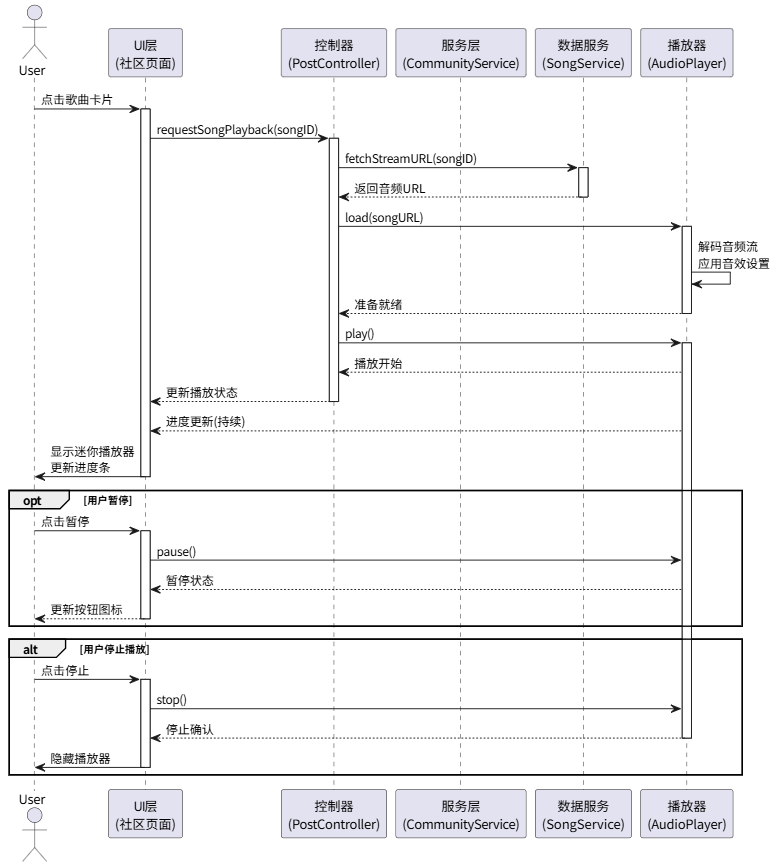
\includegraphics[width=0.9\textwidth]{images/5-1.png}
    \caption{播放歌曲-顺序图}
\end{figure}
\begin{figure}[H]
    \centering
    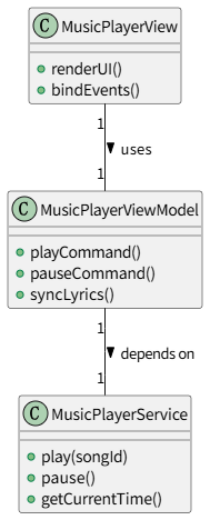
\includegraphics[width=0.3\textwidth]{images/5-2.png}
    \caption{播放歌曲-类图}
\end{figure}
\begin{figure}[H]
    \centering
    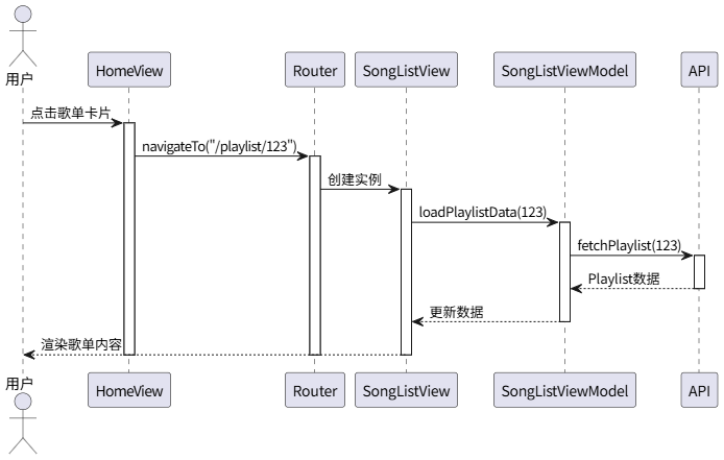
\includegraphics[width=0.9\textwidth]{images/5-3.png}
    \caption{歌单浏览-顺序图}
\end{figure}
\begin{figure}[H]
    \centering
    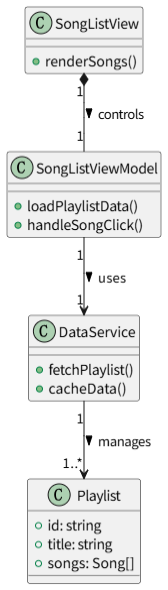
\includegraphics[width=0.2\textwidth]{images/5-4.png}
    \caption{歌单浏览-类图}
\end{figure}
\begin{figure}[H]
    \centering
    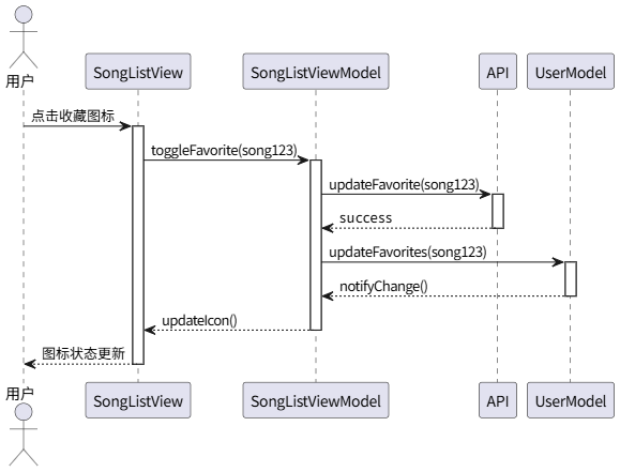
\includegraphics[width=0.9\textwidth]{images/5-5.png}
    \caption{歌曲收藏-顺序图}
\end{figure}
\begin{figure}[H]
    \centering
    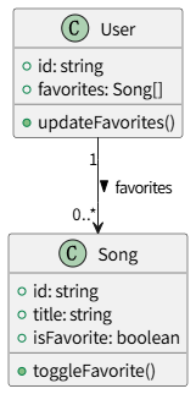
\includegraphics[width=0.2\textwidth]{images/5-6.png}
    \caption{歌曲收藏-类图}
\end{figure}
\begin{figure}[H]
    \centering
    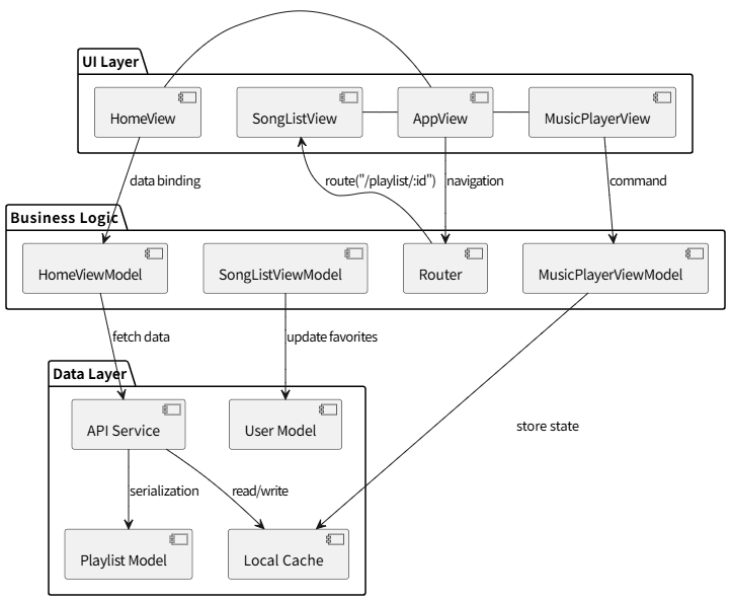
\includegraphics[width=\textwidth]{images/5-7.png}
    \caption{示意图-全局架构}
\end{figure}

\subsubsection{类设计}

\begin{figure}[H]
    \centering
    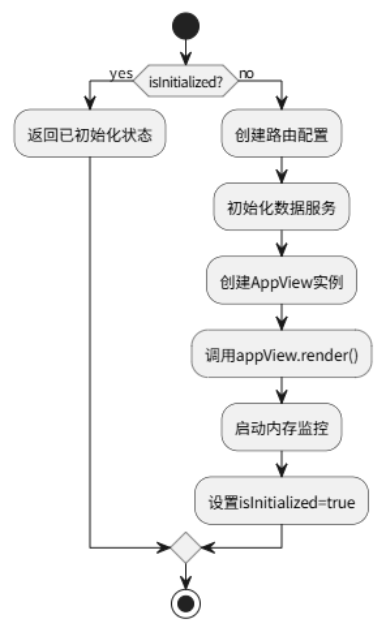
\includegraphics[width=0.4\textwidth]{images/5-8.png}
    \caption{Initialize-活动图}
\end{figure}
\begin{figure}[H]
    \centering
    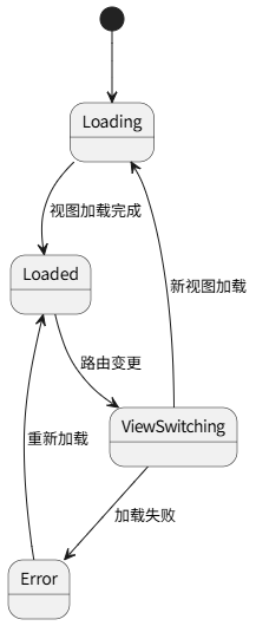
\includegraphics[width=0.25\textwidth]{images/5-9.png}
    \caption{AppView-状态图}
\end{figure}
\begin{figure}[H]
    \centering
    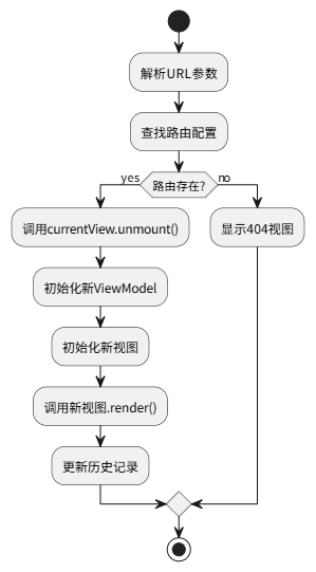
\includegraphics[width=0.25\textwidth]{images/5-10.png}
    \caption{Router-活动图}
\end{figure}

\begin{figure}[H]
    \centering
    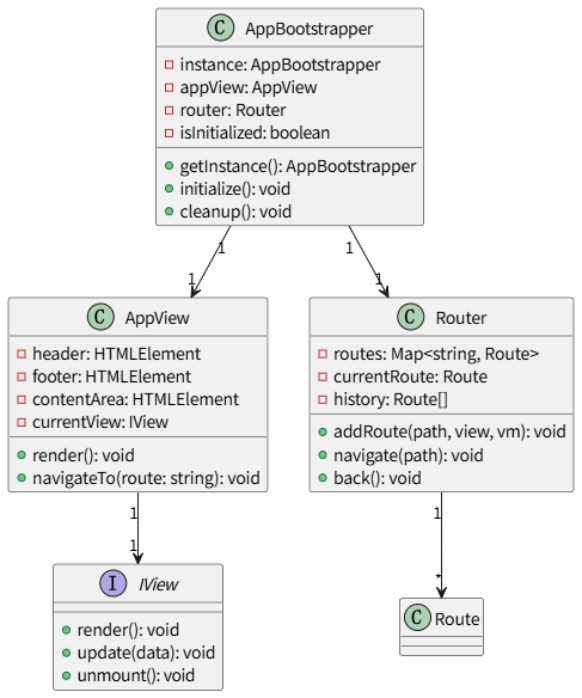
\includegraphics[width=0.7\textwidth]{images/5-11.png}
    \caption{类图}
\end{figure}

\begin{figure}[H]
    \centering
    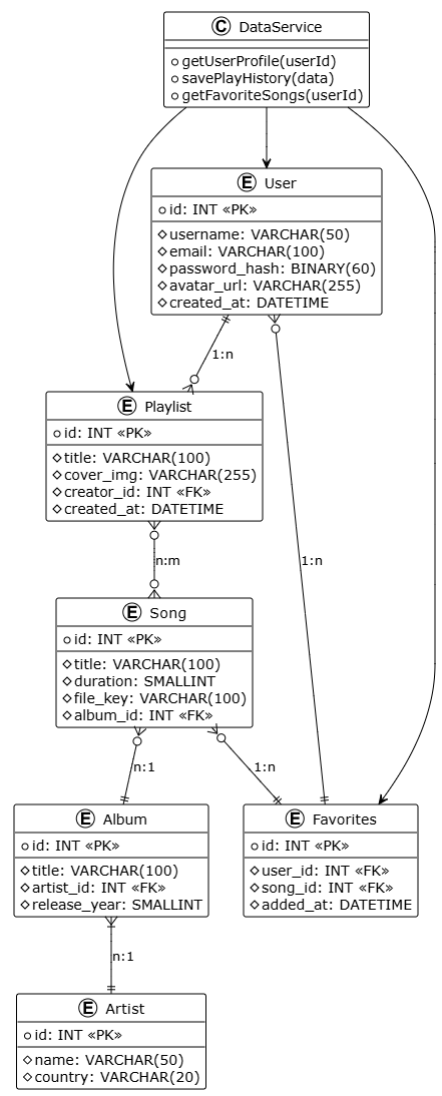
\includegraphics[width=0.5\textwidth]{images/5-12.png}
    \caption{数据库各表格类图}
\end{figure}


\subsubsection{数据设计}

\textbf{A. 概念结构设计(类图)}

\begin{figure}[H]
    \centering
    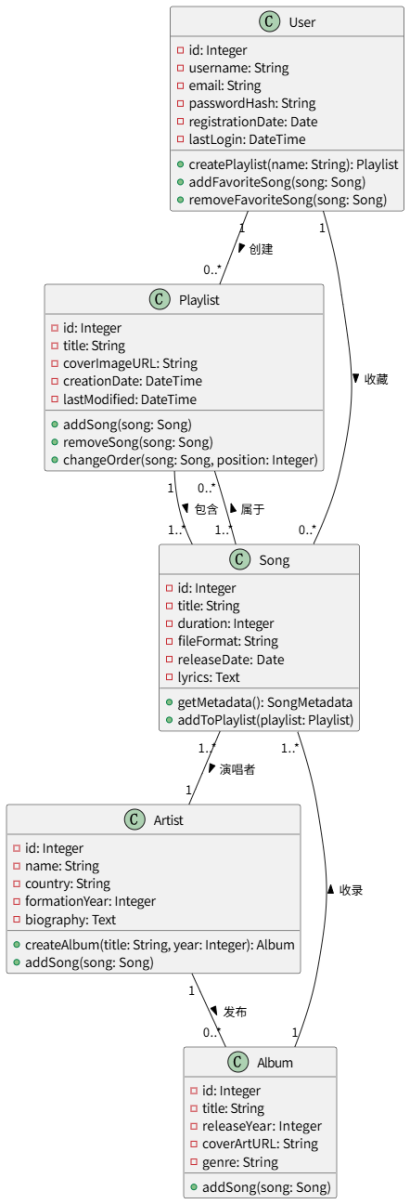
\includegraphics[width=0.5\textwidth]{images/5-14.png}
\end{figure}

\textbf{B. 逻辑结构设计}

% Please add the following required packages to your document preamble:
% \usepackage{booktabs}
% \usepackage{longtable}
% Note:It may be necessary to compile the document several times to get a multi-page table to line up properly
\begin{longtable}{@{}cccc@{}}
\caption{逻辑结构设计}
\label{tab:my-table}\\
\toprule
\textbf{关系表名}   & \textbf{字段}        & \textbf{类型}  & \textbf{约束}                     \\* \midrule
\endhead
%
\bottomrule
\endfoot
%
\endlastfoot
%
users           & user\_id           & INT          & PK, AUTO\_INC                   \\
                & username           & VARCHAR(50)  & NOT NULL, UNIQUE                \\
                & email              & VARCHAR(100) & NOT NULL, UNIQUE                \\
                & password\_hash     & CHAR(60)     & NOT NULL                        \\
                & registration\_date & DATETIME     & DEFAULT NOW()                   \\
                & last\_login        & DATETIME     &                                 \\
artists         & artist\_id         & INT          & PK, AUTO\_INC                   \\
                & name               & VARCHAR(50)  & NOT NULL                        \\
                & country            & VARCHAR(30)  &                                 \\
                & formation\_year    & YEAR         &                                 \\
                & biography          & TEXT         &                                 \\
albums          & album\_id          & INT          & PK, AUTO\_INC                   \\
                & title              & VARCHAR(100) & NOT NULL                        \\
                & release\_year      & YEAR         &                                 \\
                & cover\_art\_url    & VARCHAR(255) &                                 \\
                & genre              & VARCHAR(30)  &                                 \\
                & artist\_id         & INT          & FK (artists.artist\_id)         \\
songs           & song\_id           & INT          & PK, AUTO\_INC                   \\
                & title              & VARCHAR(100) & NOT NULL                        \\
                & duration           & SMALLINT     &                                 \\
                & file\_key          & VARCHAR(100) & NOT NULL                        \\
                & release\_date      & DATE         &                                 \\
                & lyrics             & TEXT         &                                 \\
                & album\_id          & INT          & FK (albums.album\_id)           \\
playlists       & playlist\_id       & INT          & PK, AUTO\_INC                   \\
                & title              & VARCHAR(100) & NOT NULL                        \\
                & cover\_image       & VARCHAR(255) &                                 \\
                & created\_at        & DATETIME     & DEFAULT NOW()                   \\
                & last\_modified     & DATETIME     &                                 \\
                & user\_id           & INT          & FK (users.user\_id)             \\
song\_artist    & song\_id           & INT          & PK, FK (songs.song\_id)         \\
                & artist\_id         & INT          & PK, FK (artists.artist\_id)     \\
                & is\_primary        & BOOLEAN      & DEFAULT TRUE                    \\
user\_favorites & user\_id           & INT          & PK, FK (users.user\_id)         \\
                & song\_id           & INT          & PK, FK (songs.song\_id)         \\
                & added\_at          & DATETIME     & DEFAULT NOW()                   \\
playlist\_songs & playlist\_id       & INT          & PK, FK (playlists.playlist\_id) \\
                & song\_id           & INT          & PK, FK (songs.song\_id)         \\
                & position           & SMALLINT     &                                 \\* \bottomrule
\end{longtable}

\textbf{C. 物理结构设计}

% Please add the following required packages to your document preamble:
% \usepackage{booktabs}
% \usepackage{longtable}
% Note:It may be necessary to compile the document several times to get a multi-page table to line up properly
\begin{longtable}{@{}llllll@{}}
\caption{用户信息表表}
\label{tab:my-table}\\
\toprule
\textbf{序号} & \textbf{列名} & \textbf{数据类型} & \textbf{长度} & \textbf{说明}                                                                      & \textbf{允许为空} \\* \midrule
\endhead
%
\bottomrule
\endfoot
%
\endlastfoot
%
1           & uUserId     & 文本            & 10          & \begin{tabular}[c]{@{}l@{}}用户唯一编号,主键(如 UUID 简化\\ 格式),用于身份识别与关联业务数据。\end{tabular} & 否             \\
2           & uUserName   & 文本            & 20          & \begin{tabular}[c]{@{}l@{}}用户名,登录及展示用,需符合平台\\ 命名规范。\end{tabular}                 & 否             \\
3           & uPassword   & 文本            & 15          & \begin{tabular}[c]{@{}l@{}}密码(加密存储,如 MD5/BCrypt 哈希\\ 后),保障账户安全。\end{tabular}     & 否             \\
4 & uEmail & 文本 & 10 & 用户邮箱,用于找回密码、系统通知。 & 是 \\
5 & uPhone & 文本 & 20 & 手机号码,支持快捷登录(需验证。  & 是 \\
6           & uAge        & 文本            & 整数          & \begin{tabular}[c]{@{}l@{}}年龄,0 - 100 有效范围,用于个性化\\ 推荐(如音\\ 乐风格偏好关联。\end{tabular} & 是             \\
7           & uRole       & 货币            & 文本          & \begin{tabular}[c]{@{}l@{}}用户角色(普通用户 / 创作者 / 管理员\\ 等),控制功能权限。\end{tabular}       & 否             \\* \bottomrule
\end{longtable}

% Please add the following required packages to your document preamble:
% \usepackage{booktabs}
% \usepackage{longtable}
% Note:It may be necessary to compile the document several times to get a multi-page table to line up properly
\begin{longtable}{@{}llllll@{}}
\caption{音乐作者关系表}
\label{tab:my-table}\\
\toprule
\textbf{序号} & \textbf{列名} & \textbf{数据类型} & \textbf{长度} & \textbf{说明}                                                            & \textbf{允许为空} \\* \midrule
\endhead
%
\bottomrule
\endfoot
%
\endlastfoot
%
1           & mWorkID     & 文本            & 12          & \begin{tabular}[c]{@{}l@{}}音乐作品唯一编号,主键,关联生\\ 成记录、鉴赏数据。\end{tabular}    & 否             \\
2           & mTitle      & 文本            & 50          & 作品标题,展示及检索用。                                                           & 否             \\
3           & mStyle      & 文本            & 20          & \begin{tabular}[c]{@{}l@{}}音乐风格(流行 / 古典 / 电子等),\\ 辅助推荐算法。\end{tabular} & 是             \\
4 & mGenerator & 文本 & 10  & \begin{tabular}[c]{@{}l@{}}创作者 ID(关联 tb\_user.uUserId),\\ 明确作品归属。\end{tabular} & 否 \\
5 & mInputType & 文本 & 20  & \begin{tabular}[c]{@{}l@{}}生成输入类型(文本 / 图像 / 多模态\\ 等),用于分析创作习惯。\end{tabular}    & 是 \\
6 & mFilePath  & 文本 & 255 & \begin{tabular}[c]{@{}l@{}}音乐文件存储路径(服务器 / 云存储\\ 地址),用于播放、下载。\end{tabular}      & 否 \\
7           & mCreateTime & 日期时间          & 默认          & 作品生成时间,记录创作节点。                                                         & 否             \\* \bottomrule
\end{longtable}

% Please add the following required packages to your document preamble:
% \usepackage{booktabs}
% \usepackage{longtable}
% Note:It may be necessary to compile the document several times to get a multi-page table to line up properly
\begin{longtable}{@{}llllll@{}}
\caption{音乐帖子关系表}
\label{tab:my-table}\\
\toprule
\textbf{序号} & \textbf{列名}   & \textbf{数据类型} & \textbf{长度} & \textbf{说明}                                                                             & \textbf{允许为空} \\* \midrule
\endhead
%
\bottomrule
\endfoot
%
\endlastfoot
%
1 & aAnalysisID   & 文本   & 15 & 鉴赏记录唯一编号,主键。     & 否 \\
2           & aWorkID       & 文本            & 12          & \begin{tabular}[c]{@{}l@{}}关联音乐作品 ID(tb\_music\\ \_work.mWorkID),绑定分析对象。\end{tabular}   & 否             \\
3           & aFeatureData  & 文本            & 200         & \begin{tabular}[c]{@{}l@{}}音乐特征数据(如旋律复杂度、\\ 节奏 BPM 等),JSON 格式存储,\\ 用于推荐算法。\end{tabular} & 是             \\
4           & aRecommendTag & 文本            & 50          & \begin{tabular}[c]{@{}l@{}}推荐标签(如 “治愈系”“高能量” \\ 等),辅助社区内容分发。\end{tabular}               & 是             \\
5 & aAnalysisTime & 日期时间 & 默认 & 鉴赏分析时间,记录系统处理节点。 & 否 \\* \bottomrule
\end{longtable}

% Please add the following required packages to your document preamble:
% \usepackage{booktabs}
% \usepackage{longtable}
% Note:It may be necessary to compile the document several times to get a multi-page table to line up properly
\begin{longtable}{@{}llllll@{}}
\caption{用户交互关系表}
\label{tab:my-table}\\
\toprule
\textbf{序号} & \textbf{列名} & \textbf{数据类型} & \textbf{长度} & \textbf{说明}                                                                 & \textbf{允许为空} \\* \midrule
\endhead
%
\bottomrule
\endfoot
%
\endlastfoot
%
1           & iInteractID & 文本            & 15          & 交互记录唯一编号,主键。                                                                & 否             \\
2 & iUserId & 文本 & 10 & \begin{tabular}[c]{@{}l@{}}操作用户 ID(关联\\  tb\_user.uUserId),明确交互主体。\end{tabular}                    & 否 \\
3 & iWorkID & 文本 & 12 & \begin{tabular}[c]{@{}l@{}}关联音乐作品 ID(tb\_music\_work.\\ mWorkID),若无则为社区动态\\ (如纯文字评论)。\end{tabular} & 是 \\
4           & iType       & 文本            & 10          & \begin{tabular}[c]{@{}l@{}}交互类型(评论 / 点赞 / 收藏 \\ / 私信等),区分业务逻辑。\end{tabular} & 否             \\
5           & iContent    & 文本            & 200         & \begin{tabular}[c]{@{}l@{}}交互内容(评论文字、\\ 私信消息等),需过滤敏感词。\end{tabular}         & 是             \\
6           & iCreateTime & 日期时间          & 默认          & \begin{tabular}[c]{@{}l@{}}交互发生时间,\\ 记录社区活跃节点。\end{tabular}                 & 否             \\* \bottomrule
\end{longtable}

% Please add the following required packages to your document preamble:
% \usepackage{booktabs}
% \usepackage{longtable}
% Note:It may be necessary to compile the document several times to get a multi-page table to line up properly
\begin{longtable}{@{}llllll@{}}
\caption{配置关系表}
\label{tab:my-table}\\
\toprule
\textbf{序号} & \textbf{列名}  & \textbf{数据类型} & \textbf{长度} & \textbf{说明}                                                                & \textbf{允许为空} \\* \midrule
\endhead
%
\bottomrule
\endfoot
%
\endlastfoot
%
1 & cConfigID    & 文本 & 10  & 配置项唯一编号,主键。 & 否 \\
2 & cConfigKey   & 文本 & 50  & 配置键         & 否 \\
3 & cConfigValue & 文本 & 200 & 配置值         & 是 \\
4           & cDescription & 文本            & 100         & \begin{tabular}[c]{@{}l@{}}配置说明,解释配置项作用\\ (如 “音乐生成超时时间,单位秒”)。\end{tabular} & 是             \\* \bottomrule
\end{longtable}

\subsubsection{部署设计}

\begin{figure}[H]
    \centering
    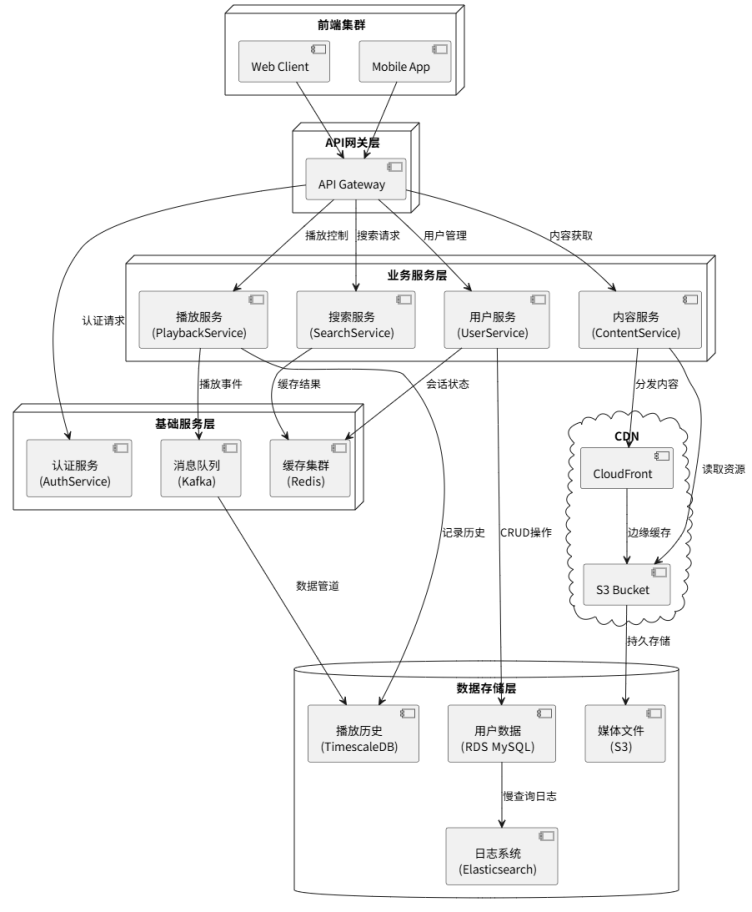
\includegraphics[width=\textwidth]{images/5-13.png}
\end{figure}

\subsubsection{系统出错处理设计}
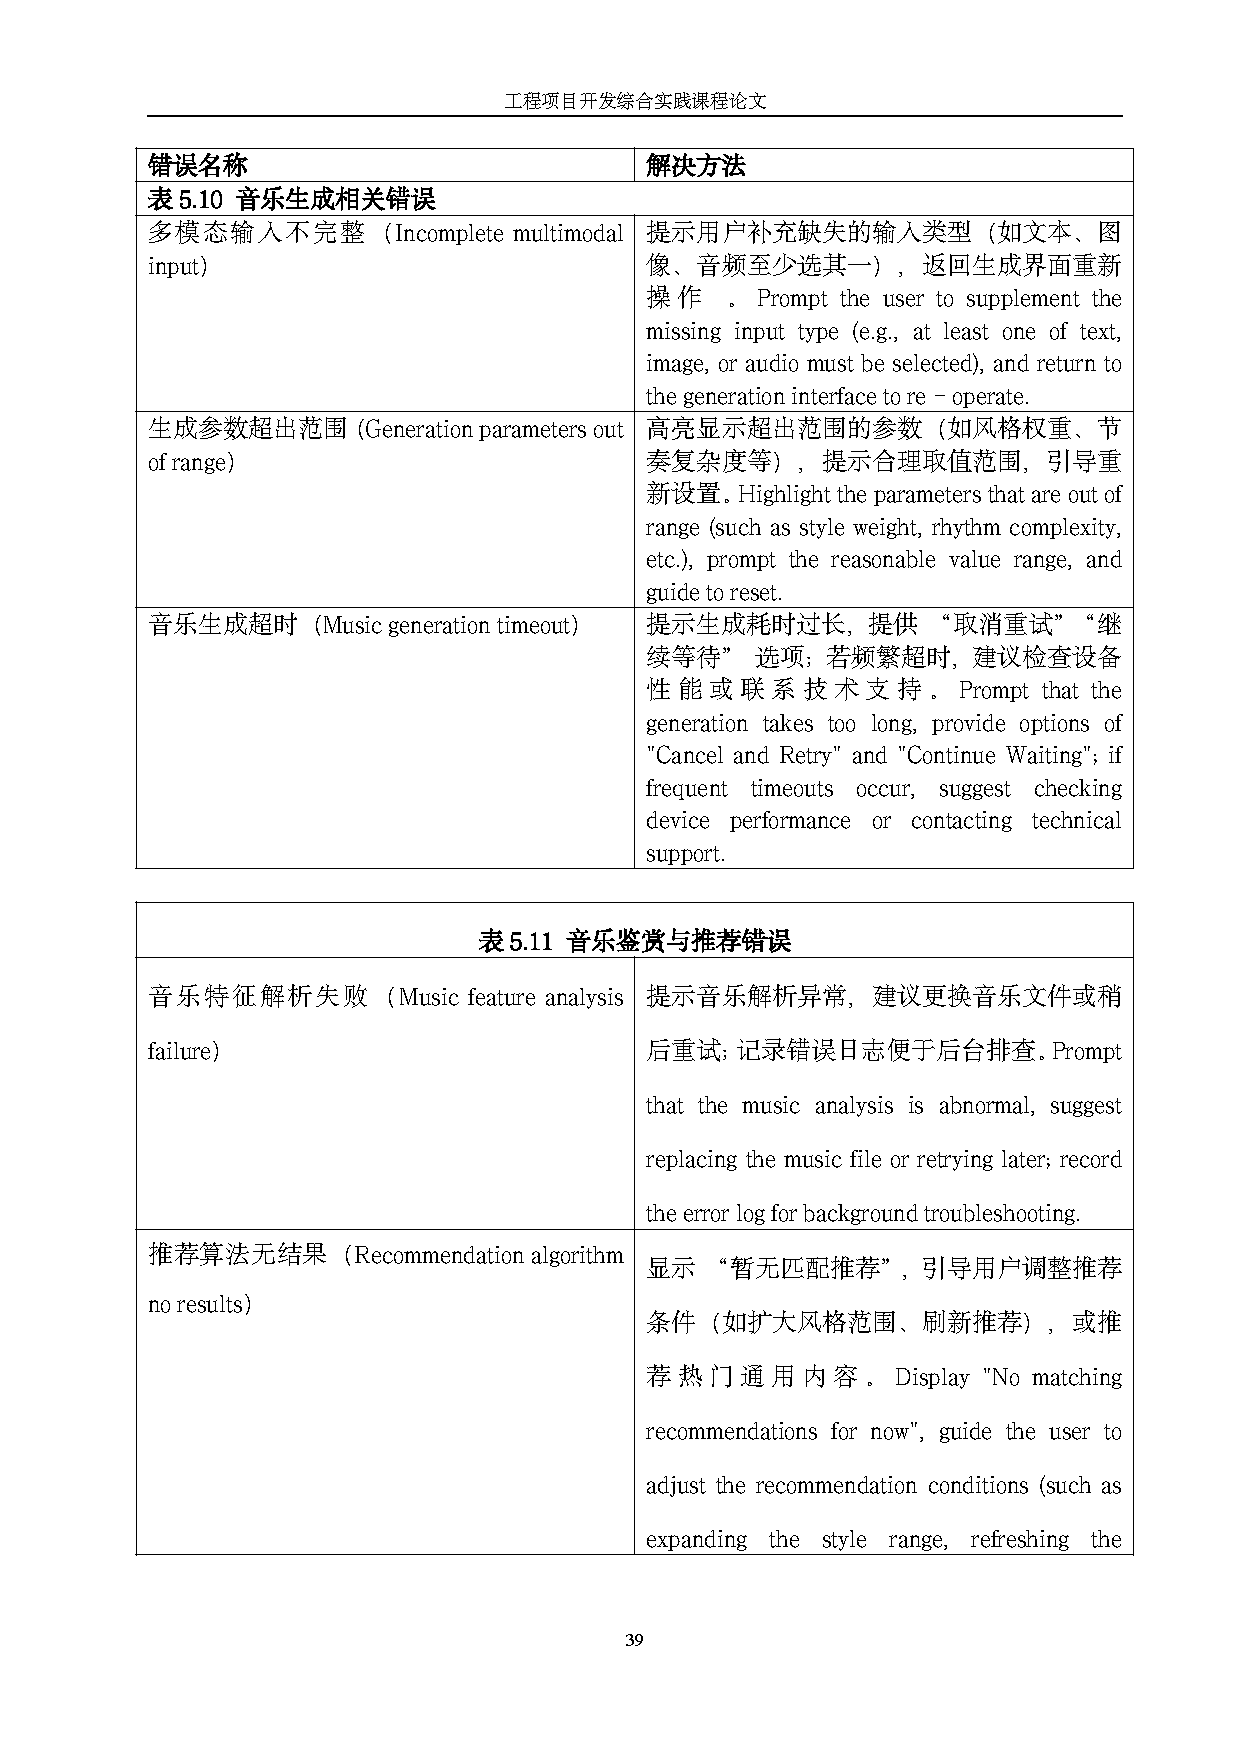
\includepdf[pages=-]{otherpdf/error_pro.pdf}

\newpage

\section{系统测试}

\subsection{引言}

本次系统测试将深度聚焦于“Music Storm”三大核心功能领域。首要目标是充分验证AI音乐生成功能的准确性和多样性,确保其能够根据用户输入有效生成风格各异、符合基本音乐规则且具有可听性的音乐片段。其次,将严格测试社区讨论平台的各项功能,包括用户注册登录、主题发布、回复互动以及个人空间管理等功能点的正确性与用户界面交互的流畅度。尤为重要的是,需针对用户发帖发表及管理员审核流程进行周密测试,确保发帖提交后能准确触发审核状态,管理员具备完整且安全的审核操作权限(通过、驳回),并且审核结果能即时反馈并呈现给相关用户,这一流程需模拟不同场景以验证其逻辑的严密性和系统的响应能力。

通过实施严谨的系统测试,我们致力于识别并排除软件中潜藏的功能性缺陷、性能瓶颈以及安全风险。测试结果将为软件质量提供客观评估,并对软件是否具备最终交付用户使用的条件做出决定性判断。系统测试的有效执行是确保“Music Storm”能够为用户提供高质量、稳定且符合期望的音乐创作与社区交流体验,从而实现项目成功的关键保障。本部分文档后续将详细阐述具体的测试策略、方法、环境及覆盖范围。

\subsection{测试概要}

% Please add the following required packages to your document preamble:
% \usepackage{booktabs}
% \usepackage{longtable}
% Note:It may be necessary to compile the document several times to get a multi-page table to line up properly
\begin{longtable}{@{}lllll@{}}
\caption{标识符及测试内容}
\label{tab:my-table}\\
\toprule
\multicolumn{1}{c}{\textbf{测试标识}} &
  \multicolumn{1}{c}{\textbf{测试内容}} &
  \multicolumn{1}{c}{\textbf{计划测试内容}} &
  \multicolumn{1}{c}{\textbf{实际测试内容}} &
  \multicolumn{1}{c}{\textbf{差异分析}} \\* \midrule
\endhead
%
\bottomrule
\endfoot
%
\endlastfoot
%
Test-Post &
  评论发布 &
  \begin{tabular}[c]{@{}l@{}}1.全字型类型\\ 测试 + 基础榜号\end{tabular} &
  \begin{tabular}[c]{@{}l@{}}1.以WiFi流量和5G\\ 信号下测试\end{tabular} &
  \begin{tabular}[c]{@{}l@{}}全字型类型过多,\\ 难以完成后续的评\\ 论审核机制\end{tabular} \\
Test-Audit    & 评论审核 & \begin{tabular}[c]{@{}l@{}}1.审接状态时\\ 间验证\end{tabular}  & \begin{tabular}[c]{@{}l@{}}1.以正经条目步骤\\ 状态\end{tabular} & 语言资源能力不足 \\
Test-Generate & 音乐生成 & \begin{tabular}[c]{@{}l@{}}1.所有音乐风\\ 格全覆盖\end{tabular} & \begin{tabular}[c]{@{}l@{}}1.以覆盖中国流行\\ 音乐\end{tabular} & 资源不足     \\* \bottomrule
\end{longtable}

\subsection{测试结果及发现}



\subsubsection{测试:发帖(Test-Post)}

通过测试发现系统中发布发帖功能实现情况良好,能够正确运行。
% Please add the following required packages to your document preamble:
% \usepackage{booktabs}
% \usepackage{longtable}
% Note:It may be necessary to compile the document several times to get a multi-page table to line up properly
\begin{longtable}{@{}lll@{}}
\caption{测试用例:发布评论;测试用例ID:post-comment}
\label{tab:my-table}\\
\toprule
\multicolumn{1}{c}{\textbf{输入操作}}                             & \multicolumn{1}{c}{\textbf{期望输出 / 响应}}                   & \multicolumn{1}{c}{\textbf{实际情况}} \\* \midrule
\endhead
%
\bottomrule
\endfoot
%
\endlastfoot
%
\begin{tabular}[c]{@{}l@{}}用户已登录,填写了\\ 评论,点击发布评论\end{tabular} &
  \begin{tabular}[c]{@{}l@{}}系统显示“评论已上传\\ ,等待管理员审核”\end{tabular} &
  \begin{tabular}[c]{@{}l@{}}系统显示“评论已上传,\\ 等待管理员审核”\end{tabular} \\
\begin{tabular}[c]{@{}l@{}}用户未登录,填写了\\ 评论,点击发布评论\end{tabular} &
  \begin{tabular}[c]{@{}l@{}}系统提示“用户未登录”\\ ,弹出登录窗口\end{tabular} &
  \begin{tabular}[c]{@{}l@{}}系统提示“用户未登录”,\\ 弹出登录窗口\end{tabular} \\
\begin{tabular}[c]{@{}l@{}}用户未登录,未填写\\ 评论,点击发布评论\end{tabular} & \begin{tabular}[c]{@{}l@{}}系统提示“不能发表空\\ 评论”\end{tabular} & 系统提示“不能发表空评论”                     \\* \bottomrule
\end{longtable}

\subsubsection{测试:审核(Test-Audit)}

通过测试发现系统中审核发帖功能实现情况良好,能够正确运行。

% Please add the following required packages to your document preamble:
% \usepackage{booktabs}
% \usepackage{longtable}
% Note:It may be necessary to compile the document several times to get a multi-page table to line up properly
\begin{longtable}{@{}lll@{}}
\caption{测试用例:评论审核;测试用例 ID:administrater}
\label{tab:my-table}\\
\toprule
\multicolumn{1}{c}{\textbf{输入操作}} & \multicolumn{1}{c}{\textbf{期望输出 / 响应}}                          & \multicolumn{1}{c}{\textbf{实际情况}}                               \\* \midrule
\endhead
%
点击通过按钮                            & \begin{tabular}[c]{@{}l@{}}评论保留到数据库中,\\ 并在评论界面显现出来\end{tabular} & \begin{tabular}[c]{@{}l@{}}评论保留到数据库中,\\ 并在评论界面显现出来\end{tabular} \\
点击不通过按钮                           & \begin{tabular}[c]{@{}l@{}}评论记录删除,\\ 发评论人收到系统提醒\end{tabular}    & \begin{tabular}[c]{@{}l@{}}评论记录删除,\\ 发评论人收到系统提醒\end{tabular}    \\* \bottomrule
\end{longtable}

\subsection{对软件功能的结论}

\subsubsection{功能:AI 创作(Test-Generate)}

\textbf{A. 能力}

该模块基于深度神经网络模型,支持通过文本描述(如“舒缓的钢琴夜曲”或“120BPM的电子舞曲”)在20秒内生成30-60秒的完整音乐片段。系统支持WAV、MP3及MIDI三种输出格式,允许用户调整生成片段的BPM(60-180范围)和音量(±6dB)。生成过程中实时显示频谱分析和进度条,完成后自动加载内置播放器,提供循环播放、片段裁剪(精度至0.1秒)及波形可视化功能。用户可将作品保存至个人库(最大存储100条),或直接发布至社区(自动关联“AI生成”标签),所有生成内容均嵌入不可篡改的数字水印以确保版权追溯。

\textbf{B. 限制}

模型训练数据限于非商业版权曲库,导致生成音乐的复杂性和专业性存在瓶颈——无法实现多声部交响乐编配或人声合成,且爵士、蓝调等即兴性强的流派生成质量显著低于专业作品。输出文件为单轨道混合音频,不支持分轨导出(如分离鼓组、贝斯声部)。系统严格拦截含特定艺术家风格描述的请求(如“披头士风格的摇滚”),并对连续生成实施限制(每小时≤10次)。此外,生成内容存在约5\%的旋律重复风险(与现有作品余弦相似度>0.82即自动终止输出)。

\subsubsection{功能:发帖(Test-Post)}

\textbf{A. 能力}

用户可在任何音乐条目(含AI生成作品)下提交文字发帖(上限500字符),支持插入时间戳标记(如“[01:23] 此段转调精彩”)实现精准段落引用。发帖编辑器提供基础格式工具(粗体、斜体、超链接),并自动识别15种主流乐器名称进行高亮。提交后系统即时触发关键词过滤(屏蔽2000+违规词)并生成带唯一ID的发帖快照。用户可通过“我的发帖”面板实时追踪状态(待审核/已公开/被驳回),公开发帖显示发布者头像、时间戳及获赞数,且支持@其他用户进行对话(触发站内通知)。

\textbf{B. 限制}

每日发帖提交上限为5条(防止灌水),且单条发帖超过72小时未审核则自动转为“已过期”状态不可重新提交。编辑器不支持富文本(如表格、代码块)、音频/视频嵌入及图片上传。时间戳标记仅精确到秒级,无法标注毫秒级细节。发帖一旦通过审核,用户仅可删除自己的发帖(限24小时内),无权编辑内容。跨时区用户可能因时间同步延迟导致发帖显示顺序错乱。

\subsubsection{功能:发帖审核(Test-Audit)}

\textbf{A. 能力}

管理员后台提供定制化审核面板:可同时播放关联音乐片段(同步时间戳定位)、查看用户历史违规记录(3个月内)、比对相似发帖库(防刷评)。审核决策(通过/驳回)需在2小时内完成,并通过系统消息通知用户(含具体条款依据,如“违反社区规范第3.2条”)。通过发帖自动关联数字指纹(SHA-256)防止篡改。

\textbf{B. 限制}

审核时效依赖人工响应,高峰时段(每日20:00-22:00)可能延迟至6小时。管理员无法修改发帖内容,仅能做二元判定(通过/驳回)。AI预筛对反讽、隐喻类文本误判率达35\%,需人工大量复核。系统不提供审核申诉渠道——被驳回发帖直接销毁不可恢复,用户需重新撰写提交。语言支持仅限于中文和英文,其他语种发帖需额外翻译工具辅助审核。

\subsection{分析摘要}
\subsubsection{能力}

经过测试,软件的核心能力得到了证实:它确实能根据用户的文字描述(比如“轻快的流行音乐”、“带点忧伤的钢琴曲”)创作出可播放的音乐片段。这满足了“AI音乐生成”这项基本且关键的功能要求。测试中,对于合理的音乐风格指令,系统都能在预期范围内完成任务,生成的音乐在技术层面(可播放、能保存、基础编辑)也达到了可用标准。这意味着软件的核心目标——让AI协助创作音乐——是实现了的。

用户可以对平台上的音乐作品(无论AI生成还是其他来源)发布自己的发帖。发帖内容能够被系统成功接收,并且用户能在个人空间里明确看到自己发帖的当前状态(尤其是标志性的“待审核”状态)。这验证了“用户能提交发帖”和“发帖状态可视化”这两项基本能力。然而,测试在理想网络条件下进行。

测试结果证实了审核机制的有效运转:它能够识别并阻挡那些明显违背社区规则的内容(如广告、侮辱性言论)。管理员能够收到待审列表并做出“通过”或“驳回”的决定,用户也能相应地收到结果通知(包括被拒时的大致原因说明,如违反了某条规则)。这保证了发帖内容的基本可控性和社区环境净化功能。

\subsubsection{缺陷和限制}

测试环境通常采用了最优的硬件配置(如高性能电脑或服务器)和稳定的网络。在实际运行中,当普通用户通过自己的设备(比如老旧电脑或手机)访问,或者服务器同时处理大量请求时,生成音乐的速度可能会明显变慢,甚至偶尔出现失败需要重试的情况。这源于实际环境的硬件性能和网络状况通常不如测试环境理想,以及难以预测的真实并发压力。

在实际运行中,尤其是在深夜、假期管理员少,或者某个热门作品突然引来大量发帖时,审核队伍就会排起长队。用户可能会经历数小时甚至更久的等待才能看到发帖状态的更新(从“待审核”变为“已公开”/“已驳回”)。

\subsubsection{建议}

发布发帖功能当前存在三个主要问题:弱网环境下提交失败率较高、草稿保存功能缺失以及状态反馈延迟。针对这些问题,我们计划实现一个草稿箱功能,当系统检测到网络断开时,会自动保存内容并提示用户"离线草稿保存成功"。该功能改进具有较高优先级,需要尽快实施。

发帖审核环节存在深夜时段审核延迟和申诉渠道缺失的问题。解决方案包括接入兼职审核员平台以在夜间自动增加审核人力,同时为被驳回的发帖添加"申诉"按钮,由高级管理员在48小时内完成复核。这些改进属于中等优先级。

AI音乐生成功能存在潜在风险,用户可能引导生成极端风格歌曲。我们将在AI生成过程中增加违禁词过滤机制,并定期更新违禁词库。一旦检测到违禁内容,系统将阻止传播并自动学习新增违禁词。该改进同样属于中等优先级。

\subsubsection{评价}

软件已基本实现核心功能的预定目标。在核心能力方面,AI 音乐生成功能能够按需创作基础风格的音乐片段,生成流程在技术上闭环运转;发帖发布功能确保用户提交内容可靠传输至系统,并明确反馈「待审状态」,满足基础内容交互要求;审核系统也初步建成了「AI拦截-人工复核-结果反馈」的有效机制,能够阻挡显著违规内容。这些均表明产品框架已稳定实现初始设计的主干功能,未出现阻断性技术硬伤(如服务崩溃或数据丢失)。尤其在关键合规性上,版权规避水印、发帖预审机制均运作正常,避免了基础法律风险。因此从核心功能实现角度,可以认为软件已达到「可运行产品」的基准交付标准。

\subsection{测试资源消耗}

总结测试工作的资源消耗数据,如工作人员的水平级别数量、机时消耗等。用于AI音乐生成的GPU服务器使用了60h。

\newpage

\section{系统用户操作手册}
\subsection{引言}

\subsubsection{编写目的}

编写本系统用户操作手册,是为了让 MusicStorm 的各类用户能快速掌握系统使用方法。无论是初次接触的普通用户,还是有专业需求的创作者,都能通过手册清晰了解音乐生成、鉴赏、社区互动等功能的操作流程,轻松完成从基础使用到高级功能探索。同时,手册也包含常见问题解答,帮助用户自主解决使用中遇到的问题,减少对技术支持的依赖,提升整体使用体验,进而增强用户对系统的认可度和使用粘性。

\subsubsection{适用范围}

本系统用户操作手册适用于所有使用 Music Storm 系统的用户,包括但不限于音乐创作者、音乐爱好者、音乐教育机构人员及文化娱乐企业用户等。无论用户是初次接触系统的新手,还是熟悉功能的进阶用户,均可通过手册获取所需信息:新手能从中学习基础操作,如注册登录、音乐生成与上传;进阶用户可参考高级功能说明,如参数自定义调节、版权交易流程;教育机构和企业用户则能借助手册指导团队成员统一规范使用系统,开展教学或创作工作。手册覆盖系统全功能模块的操作指引,适用于 PC 端及移动端等不同使用场景,为各类用户在系统使用过程中提供全面支持。

\subsubsection{版权声明}

本系统用户操作手册及所涉及的 Music Storm 系统相关内容(包括但不限于文字描述、界面截图、功能说明、操作流程等)的知识产权归新疆大学计算机科学与技术学院计算机 22 级 “入营是什么感觉” 团队所有。未经书面许可,任何单位或个人不得擅自以复制、传播、改编、翻译等任何形式使用本手册及相关内容,不得将其用于商业用途或向第三方泄露。

用户通过本手册获取的系统使用方法及相关信息,仅可用于合法使用 Music Storm 系统的目的,不得利用其从事任何违反法律法规、侵犯他人权益或违背公序良俗的活动。对于未经授权使用本手册及相关内容所造成的任何损失,开发团队保留追究法律责任的权利。

\subsection{安装与卸载}

安装 MusicStorm 系统前,需确保设备满足以下条件:操作系统为 Windows 10 及以上、macOS 10.15 及以上或 Linux(Ubuntu 20.04 及以上),内存不少于 8GB,存储空间至少 10GB,且已安装 Python 3.8 及以上版本。安装时,从官网下载对应系统的安装包,Windows 和 macOS 用户双击安装包并按向导操作,Linux 用户解压后执行bash install.sh脚本,完成后首次启动系统会自动配置依赖,生成一首测试音乐无报错即安装成功。

卸载系统时,先关闭所有相关进程。Windows 用户通过 “控制面板→程序→卸载程序” 操作,macOS 用户将应用拖至废纸篓并清空,Linux 用户运行bash uninstall.sh脚本。卸载后建议删除残留文件,默认路径为 C:/Users/ 用户名 / AppData/Roaming/MusicStorm(Windows)或~/.music-storm(macOS/Linux)。注意安装失败可尝试手动安装依赖(pip install -r requirements.txt),卸载前请导出个人作品,升级系统建议直接覆盖安装以保留数据。

\subsection{使用说明}

\subsubsection{发布功能}

\begin{figure}[H]
    \centering
    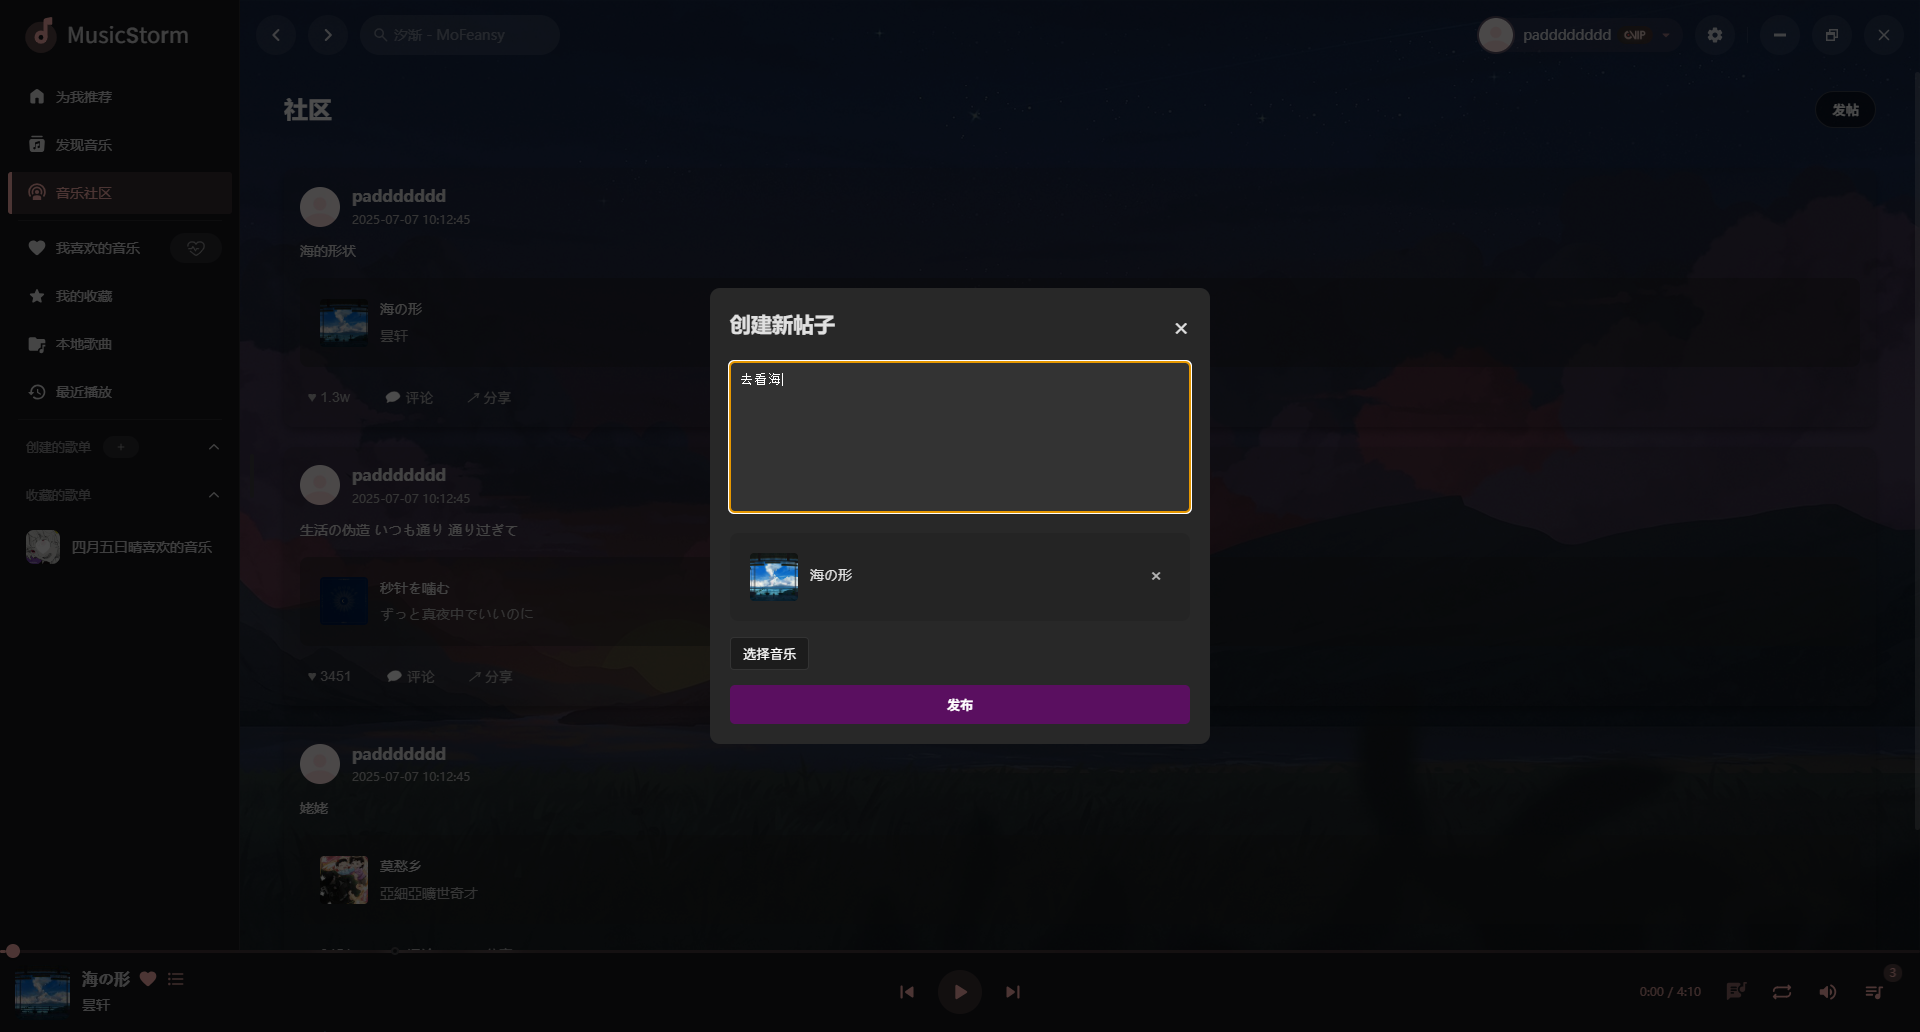
\includegraphics[width=\textwidth]{images/7-1.png}
    \caption{发布功能}
    \label{fig:post}
\end{figure}

\textbf{A. 核心数据概览功能}

核心数据概览功能是 Music Storm 系统为用户提供的一站式数据汇总与可视化工具,集中展示用户在平台内的核心创作、互动及账户相关数据,帮助用户快速掌握自身在社区中的活跃度与成果。该功能位于个人中心首页,以卡片式布局呈现关键指标,包括创作数据(如生成音乐总数、被收藏作品数量、平均生成时长)、互动数据(评论数、点赞数、粉丝增长趋势)及账户数据(注册时长、会员等级、权限状态)

数据展示支持多维度筛选与时间范围选择,用户可查看今日、本周、本月或自定义时段的统计结果,且所有数据均配有折线图、柱状图等可视化图表,直观呈现数据变化趋势。例如,创作数据区会显示不同音乐风格的作品占比,帮助用户了解自身创作偏好;互动数据区通过粉丝增长曲线,让用户清晰掌握社区影响力的变化。

此外,核心数据概览还提供数据导出功能,用户可将统计结果保存为 Excel 或 PDF 格式,用于创作复盘或成果展示。对于企业用户和教育机构,该功能还支持团队数据汇总,方便管理员查看成员整体创作与互动情况,为团队管理提供数据支持。通过这一功能,用户无需在多个模块间切换,即可全面了解自身在平台的活动轨迹与成果,提升对个人创作与社区参与的掌控感。

\textbf{B. 帖子管理功能}

帖子管理功能是 Music Storm 社区模块的核心功能之一,为用户提供对个人发布的帖子(如音乐作品分享、创作心得、话题讨论等)的全生命周期管理能力,帮助用户高效维护社区内容。

用户发布帖子后,可在 “我的帖子” 页面查看所有内容,支持按发布时间、互动热度(评论 / 点赞数)排序筛选。针对单条帖子,可执行编辑操作(修改文字描述、补充音乐附件、更新话题标签),满足内容完善需求;若内容有误或不再需要,可直接删除,删除后系统将同步清除关联的评论与互动数据,并提示 “该帖子已移除”。

对于热门帖子或需要长期展示的内容,用户可设置 “置顶”,使其在个人主页优先显示;若帖子引发不当评论,可开启 “评论审核” 模式,手动筛选待显示的评论内容,或直接关闭评论功能。此外,系统支持帖子数据追踪,在管理页展示每条帖子的浏览量、转发量及互动峰值时段,帮助用户分析内容传播效果。

针对企业或机构用户,还提供批量管理功能,可通过关键词搜索定位目标帖子,批量执行编辑、删除或隐藏操作,提升内容管理效率。所有操作均实时同步至社区动态,确保其他用户看到的内容与管理状态一致,维护社区信息的准确性与整洁度。

\textbf{C. 数据分析功能}

数据分析功能是 Music Storm 为用户和管理员提供的深度数据洞察工具,通过对平台内各类行为数据的采集、整合与可视化分析,帮助用户了解创作表现、社区互动效果及作品传播轨迹,同时为平台运营提供决策支持。​

对于普通用户,数据分析功能聚焦个人创作与互动数据。在创作维度,系统会统计用户生成音乐的总量、风格分布(如流行、古典、电子等占比)、平均生成时长及用户评分,通过饼图展示风格偏好,用折线图呈现创作频率变化,让用户清晰掌握自身创作特点与进步轨迹。互动数据方面,会汇总用户作品的总点赞数、评论量、收藏量及分享次数,按时间维度生成趋势图,直观呈现哪些作品更受社区欢迎,同时分析评论关键词,提炼用户反馈的核心观点(如 “节奏明快”“风格独特” 等),为后续创作方向提供参考。

针对社区活跃用户和创作者,数据分析功能还会深入挖掘作品传播路径,展示作品被哪些用户收藏、分享至哪些外部平台(如社交软件、音乐论坛),以及二次传播带来的新流量,帮助用户识别核心受众群体及其偏好。此外,系统会对比用户作品与同风格热门作品的各项指标(如互动率、播放完成率),找出差距并给出优化建议,例如 “您的电子风格作品平均播放完成率低于同类作品 15\%,建议缩短前奏时长”。​

对于管理员和机构用户,数据分析功能覆盖平台整体运营数据,包括日活跃用户数、新增注册用户趋势、各功能模块使用频率(如音乐生成、社区互动、版权交易等),通过仪表盘实时展示核心指标。同时,会分析用户留存率(新用户 7 日留存、月留存)、创作转化率(浏览用户中实际生成音乐的比例),并关联不同推广活动与数据变化,评估活动效果。在内容监管方面,还能统计违规内容类型及处理效率,为社区规范调整提供依据。​

所有数据分析结果均以图表(柱状图、折线图、热力图等)结合文字解读的形式呈现,支持按日、周、月、自定义时段筛选数据,且提供数据导出功能(支持 Excel、CSV 格式)。用户可根据自身需求灵活选择分析维度,无论是普通用户复盘创作成果,还是管理员优化平台运营,都能通过该功能快速获取有价值的信息,实现数据驱动的决策与成长。

\textbf{D. 消息管理系统}

消息管理系统是 Music Storm 社区交互的核心功能之一,集中处理用户在平台内的各类消息通知,帮助用户高效接收、筛选和管理互动信息,避免遗漏重要内容。
该系统整合了多种消息类型,包括互动通知(如作品被点赞、评论、收藏,收到新粉丝关注)、系统通知(如功能更新提醒、活动邀请、权限变动)、私信消息(用户间一对一对话)及团队消息(加入的音乐主题小组内的公告或讨论)。所有消息统一展示在 “消息中心”,按类型分为不同标签页,用户可快速切换查看,也可通过顶部搜索栏按关键词(如发送者昵称、消息内容)精准定位。

针对高频消息,系统支持自定义提醒设置:用户可开启或关闭某类消息的推送(如关闭点赞通知),选择通知方式(弹窗、铃声、桌面提醒),并设置免打扰时段(如夜间 10 点至次日 7 点),减少不必要的干扰。对于重要消息,可标记为 “未读” 或 “星标”,星标消息会单独归类,方便后续优先处理;已读消息可批量删除或归档,保持消息列表整洁。

私信功能支持实时对话,包含文字、表情、音乐片段分享,用户可设置 “陌生人私信权限”(允许所有人、仅关注者或拒绝),并可将骚扰消息举报至系统审核。消息中心还会显示未读消息总数,且在移动端支持消息推送,确保用户即使未登录系统,也能及时获取关键互动信息。

通过消息管理系统,用户既能全面掌握社区内的互动动态,又能自主控制消息接收节奏,平衡社交参与与使用体验,增强对平台的使用粘性。

\textbf{E. 远程监控功能}

远程监控功能是 Music Storm 系统为管理员和机构用户提供的运维与安全管理工具,通过实时追踪系统运行状态、用户行为及内容合规性,保障平台稳定运营与社区环境健康。
该功能支持管理员在异地通过授权账号登录监控后台,实时查看核心服务器的性能指标(如 CPU 使用率、内存占用、网络带宽),当指标超出预设阈值(如 CPU 持续 5 分钟超 80\%)时,系统自动触发告警(弹窗 + 短信通知),便于及时排查故障(如服务器过载、异常请求攻击)。同时,可监控多终端(PC 端、移动端)的服务响应速度,定位某一地区或设备类型的访问延迟问题,辅助优化网络部署。​

在用户行为监控方面,功能聚焦异常操作识别,如短时间内频繁生成音乐(可能触发刷量)、批量发布相似内容(疑似垃圾信息)、跨账号高频互动(涉嫌刷数据)等,系统会标记此类行为并生成风险报告,管理员可手动审核或设置自动处理规则(如限制账号功能、临时禁言)。对于内容安全,远程监控会实时扫描新发布的帖子、评论及私信,通过关键词库与 AI 识别模型筛查违规内容(如侵权音乐、不良言论),发现后立即拦截并通知审核人员处理,避免违规信息扩散。​

监控数据以实时仪表盘形式呈现,包含服务器状态看板、用户行为风险清单、内容合规率统计等模块,支持按时间轴回溯历史数据(如过去 24 小时的告警记录、违规处理结果),并生成周 / 月运营报告。管理员可自定义监控范围(如重点关注某一功能模块、特定用户群体),设置分级告警机制(如紧急故障直接联系负责人,一般异常仅记录日志),平衡监控精度与运维效率。​

需注意,该功能严格遵循数据隐私规范,仅对管理员开放经授权的监控权限,用户个人信息(如手机号、地址)会脱敏处理,且所有监控操作均留有日志存档,确保合规可追溯。通过远程监控,管理员无需现场值守即可全面掌控平台运行状况,快速响应异常情况,为系统稳定与社区安全提供持续保障。

\textbf{F. 内容运营功能}

支持短视频内容发布与流量分析并实时显示内容传播效果,通过评论内容分析用户偏好。

\newpage

\subsubsection{审核功能}

\begin{figure}[H]
    \centering
    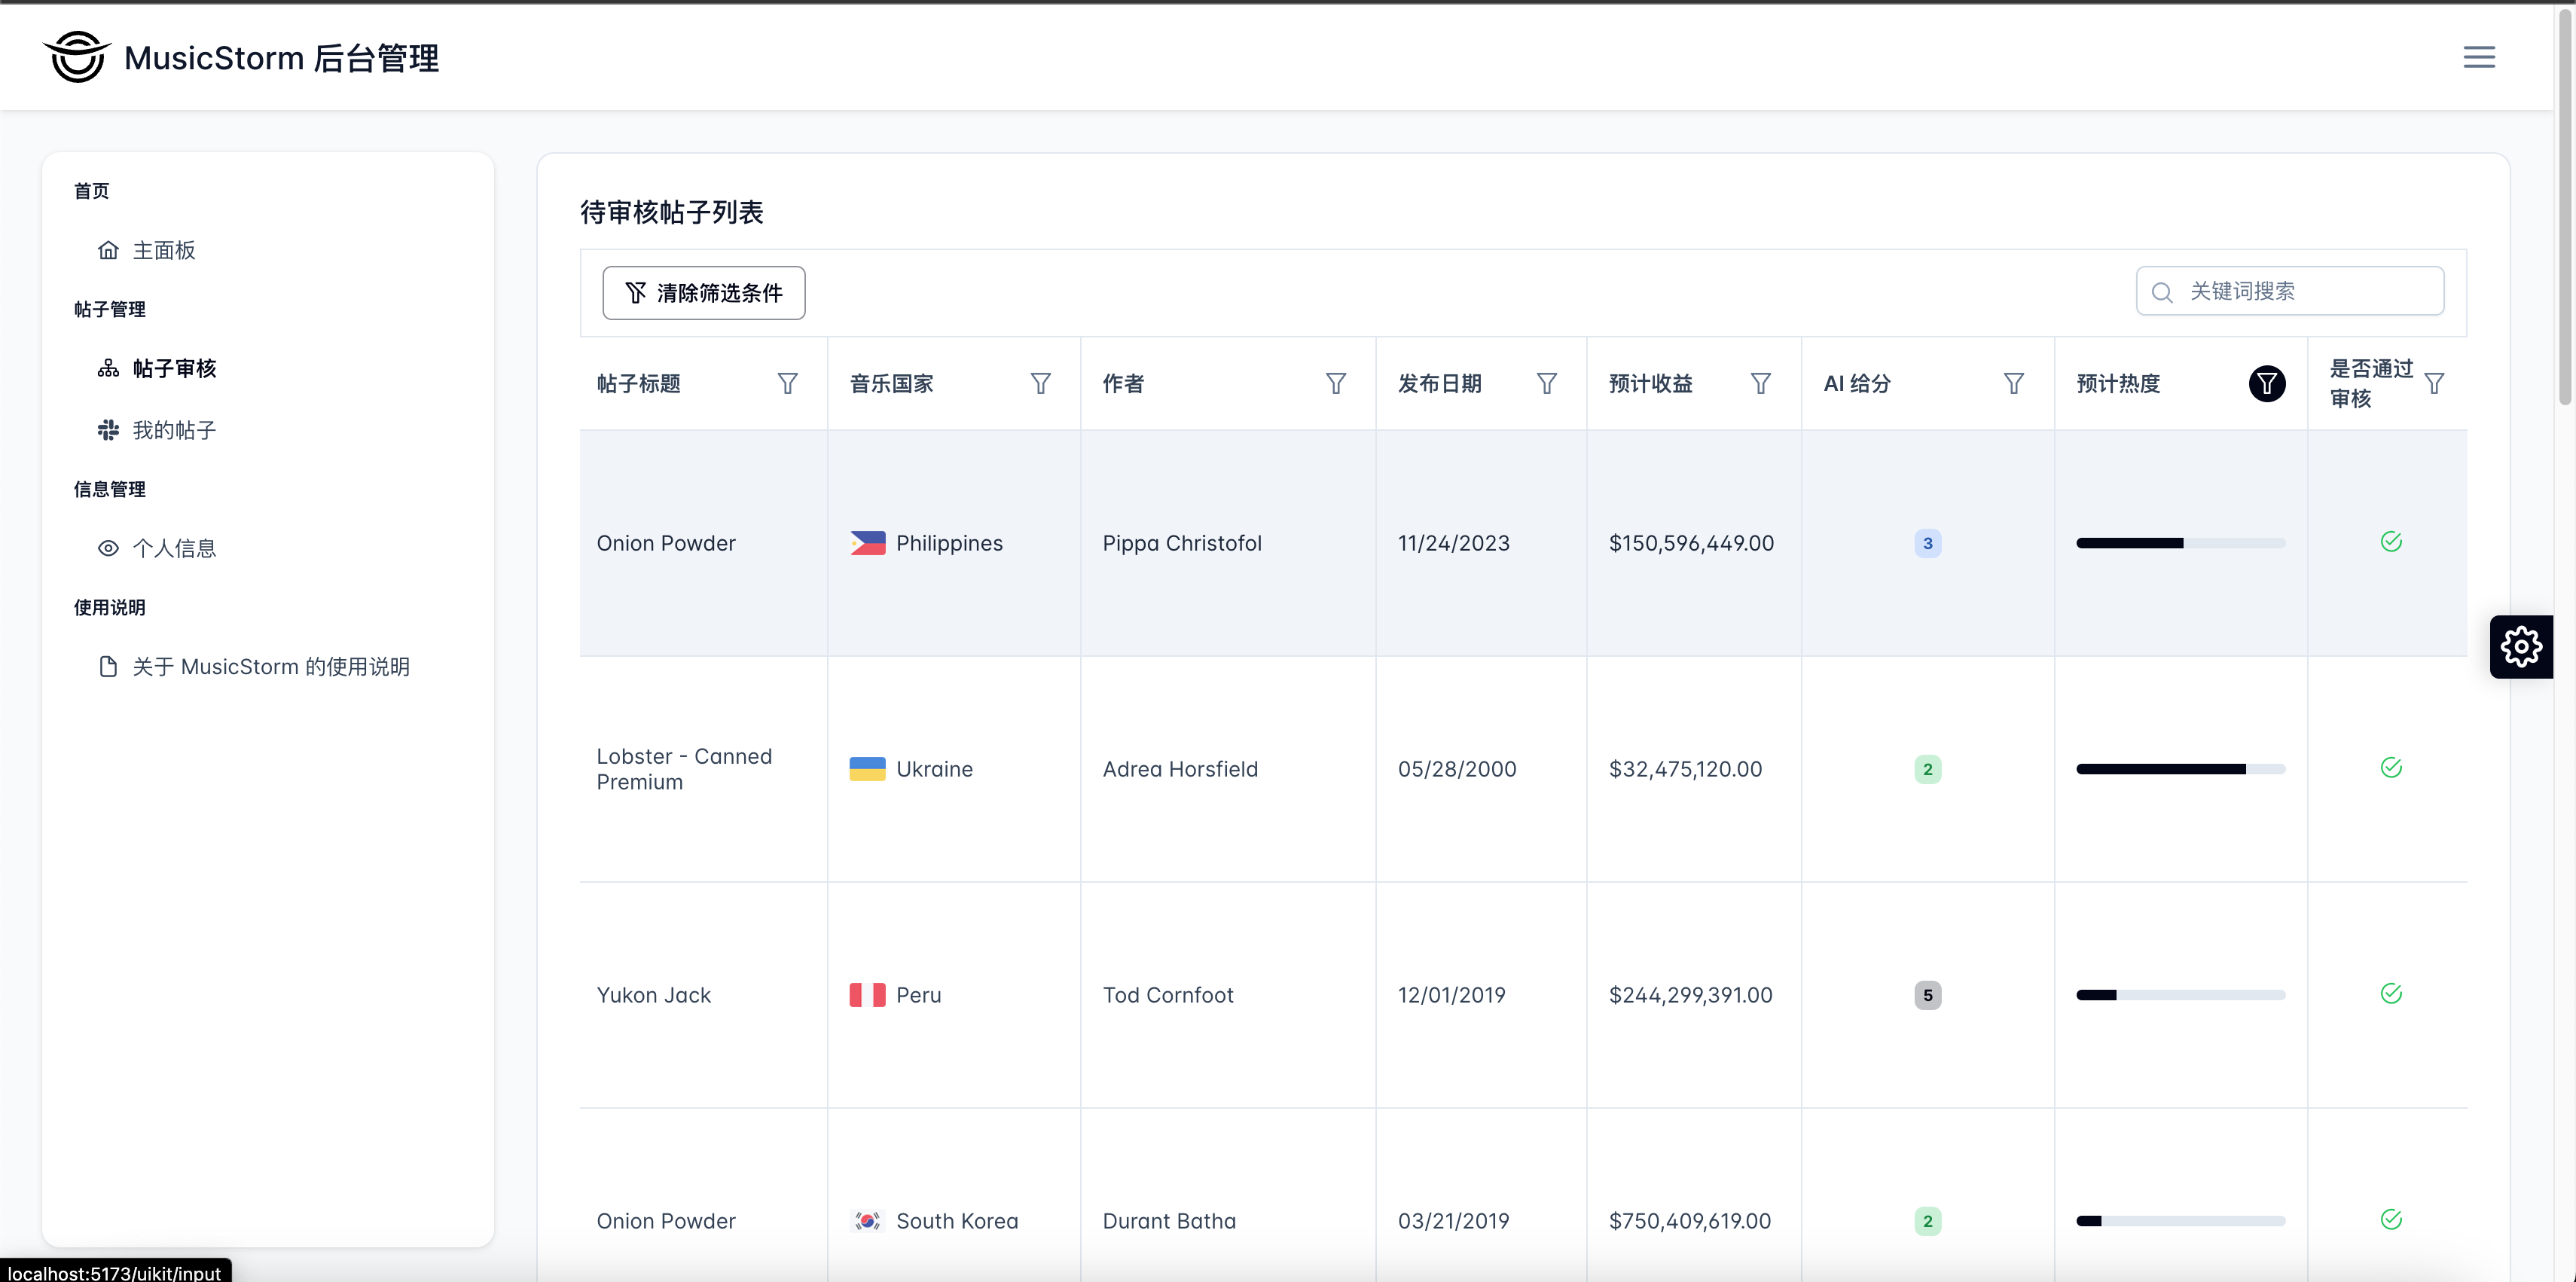
\includegraphics[width=\textwidth]{images/7-3.png}
    \caption{审核功能}
    \label{fig:review}
\end{figure}

\textbf{A. 待审帖子列表管理功能}

待审帖子列表管理功能是内容审核环节的核心模块,用于集中展示经系统自动筛查后标记为 “疑似违规” 的帖子,方便管理员高效处理待审内容。

该列表按 “提交时间” 倒序排列(最新待审帖子优先显示),每条待审条目包含帖子标题、发布者昵称、提交时间、疑似违规类型(如 “含敏感词”“版权存疑”)及风险等级(高 / 中 / 低),风险等级由系统根据违规概率自动判定,高风险帖子以红色边框标注,便于管理员优先处理。

列表支持多维度筛选:可按 “违规类型”(如文本违规、音频侵权、图片不当)快速定位特定问题帖子;通过 “风险等级” 筛选,聚焦高优先级审核任务;输入 “发布者 ID” 或 “帖子关键词”,能精准查找目标内容。此外,支持批量操作,勾选多条帖子后,可执行 “批量通过”“批量驳回”(需选择预设驳回理由)或 “批量移至复审”(适用于争议内容),大幅提升审核效率。

点击单条帖子条目,可展开查看完整内容(包括文字、音频、图片附件)及系统自动识别的违规点标注(如敏感词标红、版权比对结果),管理员结合人工判断后,点击 “通过” 则帖子即时发布,点击 “驳回” 需填写具体原因(支持关联至违规规则库),操作后系统会自动通知发布者并同步更新帖子状态至 “已处理”。列表顶部实时显示 “待审总数”“今日已处理数” 及 “平均处理时长”,帮助管理员掌握审核进度,确保待审内容及时清零。

\textbf{B. 交互功能}

审核功能的交互设计聚焦于简化管理员操作流程、强化审核决策效率及完善用户反馈机制,核心交互场景贯穿审核全流程:​

在待审内容处理环节,管理员进入 “待审核队列” 后,每条内容卡片支持悬停预览(无需点击即可查看标题、发布者及违规点摘要),点击卡片展开详情页时,系统会自动定位 AI 标记的违规片段(如文本敏感词标红、音频侵权片段高亮),并提供 “快速通过”“一键驳回” 按钮。若需进一步核验,详情页右侧设有 “资料面板”,可直接跳转至发布者历史内容、违规记录及关联作品,辅助判断是否为恶意发布。​

针对争议内容,交互功能支持 “审核合议” 触发 —— 点击详情页底部 “发起合议”,系统自动推送内容至 3 名指定审核员账号,并在其工作台生成待处理提醒;合议过程中,审核员可通过内置评论区实时标注争议点(如 “此处歌词疑似违规但无明确依据”),最终按多数票结果自动同步处理状态,避免单人决策偏差。​

对管理员与用户的双向反馈,交互功能设计了分层通知机制:管理员驳回内容时,系统提供 “驳回理由模板库”(如 “涉及版权问题”“包含敏感信息”),选择后可补充自定义说明,提交后自动生成站内信推送至用户,同时在用户发布页显示 “审核未通过” 标识及修改指引(如 “请替换侵权音频后重新提交”)。若用户对驳回结果有异议,可通过内容详情页的 “申诉” 按钮提交说明,申诉请求会实时进入管理员 “待处理申诉” 列表,并以橙色标签突出显示。
​
批量操作交互上,支持 “全选 - 筛选 - 处理” 三步式流程:勾选多条内容后,筛选框可按违规类型、风险等级二次过滤,确认后点击 “批量处理”,系统弹出操作确认弹窗(显示处理数量及影响范围),并提供 “撤销操作” 缓冲期(操作后 10 秒内可取消),减少误操作风险。​

此外,交互功能包含进度追踪与状态反馈:审核队列顶部实时显示 “待处理数 / 今日完成数”,每条内容处理后立即更新状态标签(“已通过” 为绿色、“已驳回” 为红色),并在页面右侧生成 “处理动态流”,记录操作人、时间及结果,便于团队协作追溯。通过轻量化交互设计,既降低管理员操作成本,又保障审核决策的准确性与用户对结果的感知度。

\textbf{C. 审核工作流功能}

审核工作流功能是 Music Storm 系统规范内容审核流程、保障审核质量的核心机制,通过标准化的流程设计,实现从内容提交到结果反馈的全链路自动化与可控化,确保每一条待审内容都能按规则高效流转。​

该工作流以 “分级审核 + 自动流转” 为核心逻辑,起始于用户发布内容的瞬间:当用户提交帖子、评论或音乐作品后,系统会先触发 “一级预审”—— 由 AI 审核模型自动扫描内容(文本匹配关键词库、音频比对版权库、图片检测合规性),并根据违规风险等级(高 / 中 / 低)分配流转路径。低风险内容(如无明显违规痕迹)直接通过预审,自动发布;中风险内容(如疑似敏感词但需人工确认)进入 “普通审核队列”,等待管理员处理;高风险内容(如明确包含违规信息)则进入 “加急审核通道”,并即时向在线管理员发送弹窗提醒,确保优先处理。​

在人工审核环节,工作流支持 “多级复核” 机制。普通审核队列的内容由一线审核员处理,若审核员标记 “存在争议”(如难以判定是否侵权),内容会自动流转至 “二级复核队列”,由资深审核员或审核组长进行二次判定;二级复核仍存疑的内容,将触发 “终级审议”,系统自动汇总相关证据(如 AI 检测报告、历史类似案例处理结果),提交至审核委员会,通过多人合议后给出最终结论。每一级审核节点均设有明确的处理时限(如普通审核 4 小时内、加急审核 1 小时内),超时未处理的内容会自动升级流转,并向对应审核人员发送超时提醒。​

对于特殊类型的内容(如官方合作作品、活动参赛作品),工作流支持 “定向审核” 配置。管理员可在发布规则中预设 “指定审核员”,此类内容提交后会跳过公共队列,直接分配给预设人员处理,且审核过程中可开启 “协作模式”—— 审核员之间能实时标注疑问点、共享参考资料,处理结果需所有指定人员确认后才生效,避免单人操作疏漏。​

工作流的收尾环节聚焦于结果同步与记录留存。无论审核通过、驳回还是退回修改,系统都会自动生成 “审核结果单”,包含处理意见、依据的规则条款及操作人信息,并同步至三个端口:用户端会收到清晰的结果通知(如 “您的作品因包含侵权音频未通过审核,可修改后重新提交”);审核后台会更新内容状态(通过 / 驳回 / 待修改),并将结果关联至发布者的信用积分体系;管理后台则生成 “审核日志”,记录全流程节点(提交时间、预审结果、各审核环节处理人及时间),支持按内容 ID、审核时间或处理结果追溯,为合规审计提供完整依据。

此外,工作流还具备 “流程配置灵活性”,管理员可通过 “工作流编辑器” 自定义审核节点(如增减复核层级)、调整风险等级阈值(如将原中风险的判定标准从 “60\%-80\% 违规概率” 调整为 “50\%-75\%”),并设置特殊场景的例外规则(如节假日期间自动延长审核时限),使审核流程能适配平台不同阶段的运营需求。通过这套标准化、可追溯的工作流,系统既能确保审核效率,又能最大限度减少人为误差,为社区内容安全提供坚实保障。​

\textbf{D. 批量处理功能}

批量处理功能是审核工作流中提升效率的关键工具,专为处理大量待审内容设计,支持管理员对多条待审帖子同时执行标准化操作,大幅减少重复劳动。​
该功能的触发入口位于待审帖子列表页,管理员可通过三种方式选定目标内容:直接勾选列表中的单条或多条帖子;点击 “全选” 按钮选中当前页所有内容;通过筛选条件(如 “违规类型 = 敏感词”“风险等级 = 低”)批量定位后,一键选中符合条件的帖子。选中后,列表底部会自动显示选中数量及 “批量处理” 按钮,点击后弹出操作菜单。​
可执行的批量操作包括四类核心功能:“批量通过” 适用于确认无违规的内容,操作后帖子即时发布,状态同步更新为绿色 “已通过”;“批量驳回” 需从预设理由库(如 “包含低俗信息”“涉及广告营销”)中选择驳回原因,支持补充自定义说明,提交后系统自动向发布者推送统一格式的驳回通知;“批量标记复审” 针对存在轻微争议的内容,将其转移至 “复审队列” 并标注优先级,便于资深审核员集中处理;“批量暂存” 可将选中内容移至 “待处理缓冲区”,暂时退出当前审核队列,待后续空闲时重新调出处理,避免因信息不全导致误判。​
为确保操作精准性,批量处理配备多层筛选机制。选中内容后,可通过二次筛选框按 “发布时间”“发布者等级”“内容类型(文字 / 音频 / 图文)” 进一步缩小范围,例如在已选中的 100 条 “敏感词” 违规帖子中,筛选出 “24 小时内提交” 且 “发布者为新用户” 的内容单独处理。操作前,系统会弹出确认弹窗,清晰展示选中数量、涉及的风险等级分布及操作影响(如 “本次批量通过将使 30 条内容即时可见”),并提供 10 秒 “撤销倒计时”,防止误操作。​


\textbf{E. 数据可视化功能}

审核功能的数据可视化模块是辅助管理员掌握审核全局、优化工作效率的直观工具,通过图表整合与动态展示,将复杂的审核数据转化为可快速解读的视觉信息。​
该功能的核心展示区位于审核工作台首页,以 “审核数据总览仪表盘” 为中心,聚合三大类关键指标:实时数据(当前待审量、审核中数量、今日已处理总量)以动态数字牌呈现,配合进度条显示积压率(如 “待审量 120 条,积压率 25\%”);趋势数据通过折线图展示近 7 天审核量变化,横轴为日期,纵轴为处理条数,可切换 “按小时”“按天” 粒度,清晰呈现流量高峰时段(如每日 19-21 点为审核高峰);结果分布数据则用环形图展示 “通过”“驳回”“复审”“暂存” 四类结果的占比,点击图例可单独高亮某一类别,同时显示对应数量及占比详情(如 “驳回占比 30\%,其中 60\% 因敏感词违规”)。​

针对细分维度,数据可视化提供多维度下钻功能。在 “违规类型分析” 板块,柱状图按违规类型(敏感词、版权侵权、低俗内容等)展示数量分布,鼠标悬停可查看该类型的日均处理量、平均审核时长及典型案例;“审核效率分析” 通过雷达图对比不同审核员的处理速度、准确率(驳回正确率、复审一致率),帮助识别效率瓶颈;“用户申诉分析” 则用折线图呈现近 30 天申诉量与申诉成功率,关联显示申诉通过的主要原因(如 “审核误判”“规则更新”)。​

交互设计上,支持自定义筛选与联动分析。管理员可通过时间筛选器(今日 / 本周 / 本月 / 自定义)调整数据范围,选择 “仅显示加急审核”“仅看新用户内容” 等条件后,所有图表会实时同步更新;点击某一图表的关键数据点(如折线图中的峰值点),系统会自动联动展示该时段的详细审核记录列表,便于追溯异常原因(如 “7 月 5 日 19 点审核量骤增,因平台活动导致新帖爆发”)。​

功能支持数据导出与定期报告生成。点击仪表盘右上角 “导出” 按钮,可将当前图表及原始数据保存为 Excel 或图片格式;设置 “自动报告” 后,系统会按日 / 周生成审核数据简报,包含核心指标、异常波动分析及优化建议(如 “建议在 19 点前增加审核人力”),自动推送至管理员邮箱或工作台,为审核资源调配与规则优化提供数据支撑。通过数据可视化,管理员无需解读复杂数据表格,即可快速把握审核工作节奏、识别潜在问题,实现从 “被动处理” 到 “主动优化” 的转变。

\textbf{F. 热度预测模型}

热度预测模型是审核功能中辅助资源调配的智能化工具,通过算法分析待审内容的潜在传播力,提前预判其发布后的热度等级,帮助审核团队优先处理高潜力内容,平衡审核效率与社区活跃度。​

该模型的核心逻辑是基于内容特征与用户行为数据构建预测算法。数据来源涵盖两方面:一是内容本身属性,包括标题关键词(如 “热门话题词”“争议性词汇”)、发布者历史表现(粉丝量、过往作品平均互动率)、内容类型(音乐作品 / 话题讨论 / 创作教程)及附件特征(音频时长、图片数量);二是平台历史数据,通过学习近 3 个月内同类内容的传播轨迹(如发布后 1 小时 / 24 小时的浏览量、转发量峰值),建立特征与热度的关联模型。​
预测维度分为三级热度标签:“高热度潜力”(预计 24 小时内浏览量超 10 万、互动率≥8\%)、“中热度潜力”(预计浏览量 3 万 - 10 万、互动率 3\%-8\%)、“低热度潜力”(预计浏览量低于 3 万、互动率<3\%)。模型会在待审内容进入队列时自动生成预测结果,并在待审列表中以对应颜色标签标注(红色为高热度、黄色为中热度、灰色为低热度),同时显示预测依据(如 “含 \#电子音乐挑战\# 热门话题,发布者过往作品平均互动率 12\%”)。​

在审核流程中,热度预测模型与优先级机制深度联动。高热度潜力内容会自动进入 “优先审核通道”,即使风险等级为中低,也会被标记为 “需快速处理”,确保优质高潜力内容尽快发布抢占流量窗口;对于高风险但预测热度高的内容(如含争议话题的爆款潜质帖子),模型会提示 “高风险高热度”,触发 “双人复核” 机制,避免因误判错失优质内容或放行违规内容引发不良影响。​

模型还支持动态调整与效果反馈。每日会自动对比预测热度与实际传播数据,计算预测准确率(如高热度标签内容的实际达标率),并基于偏差值迭代算法参数(如调整 “发布者粉丝量” 的权重占比);管理员可在 “模型设置” 中查看近 7 天的预测准确率报告,手动校准特殊场景的预测逻辑(如节假日期间热门话题的权重调整)。​

应用场景上,热度预测模型为审核排班提供数据支撑。通过汇总每日待审内容的热度预测分布(如预计次日高热度内容占比 30\%),系统会自动生成审核人力调配建议(如 “明日 10-12 点高热度内容集中,建议增加 2 名审核员”);同时,对预测为高热度但因违规被驳回的内容,会向运营团队推送 “潜在热点缺口” 提示,辅助策划替代话题,维持社区热度稳定。通过热度预测模型,审核功能从 “被动处理” 升级为 “主动预判”,在保障内容合规的前提下,最大化释放优质内容的传播价值。


\subsubsection{AI 音乐生成功能}

\begin{figure}[H]
    \centering
    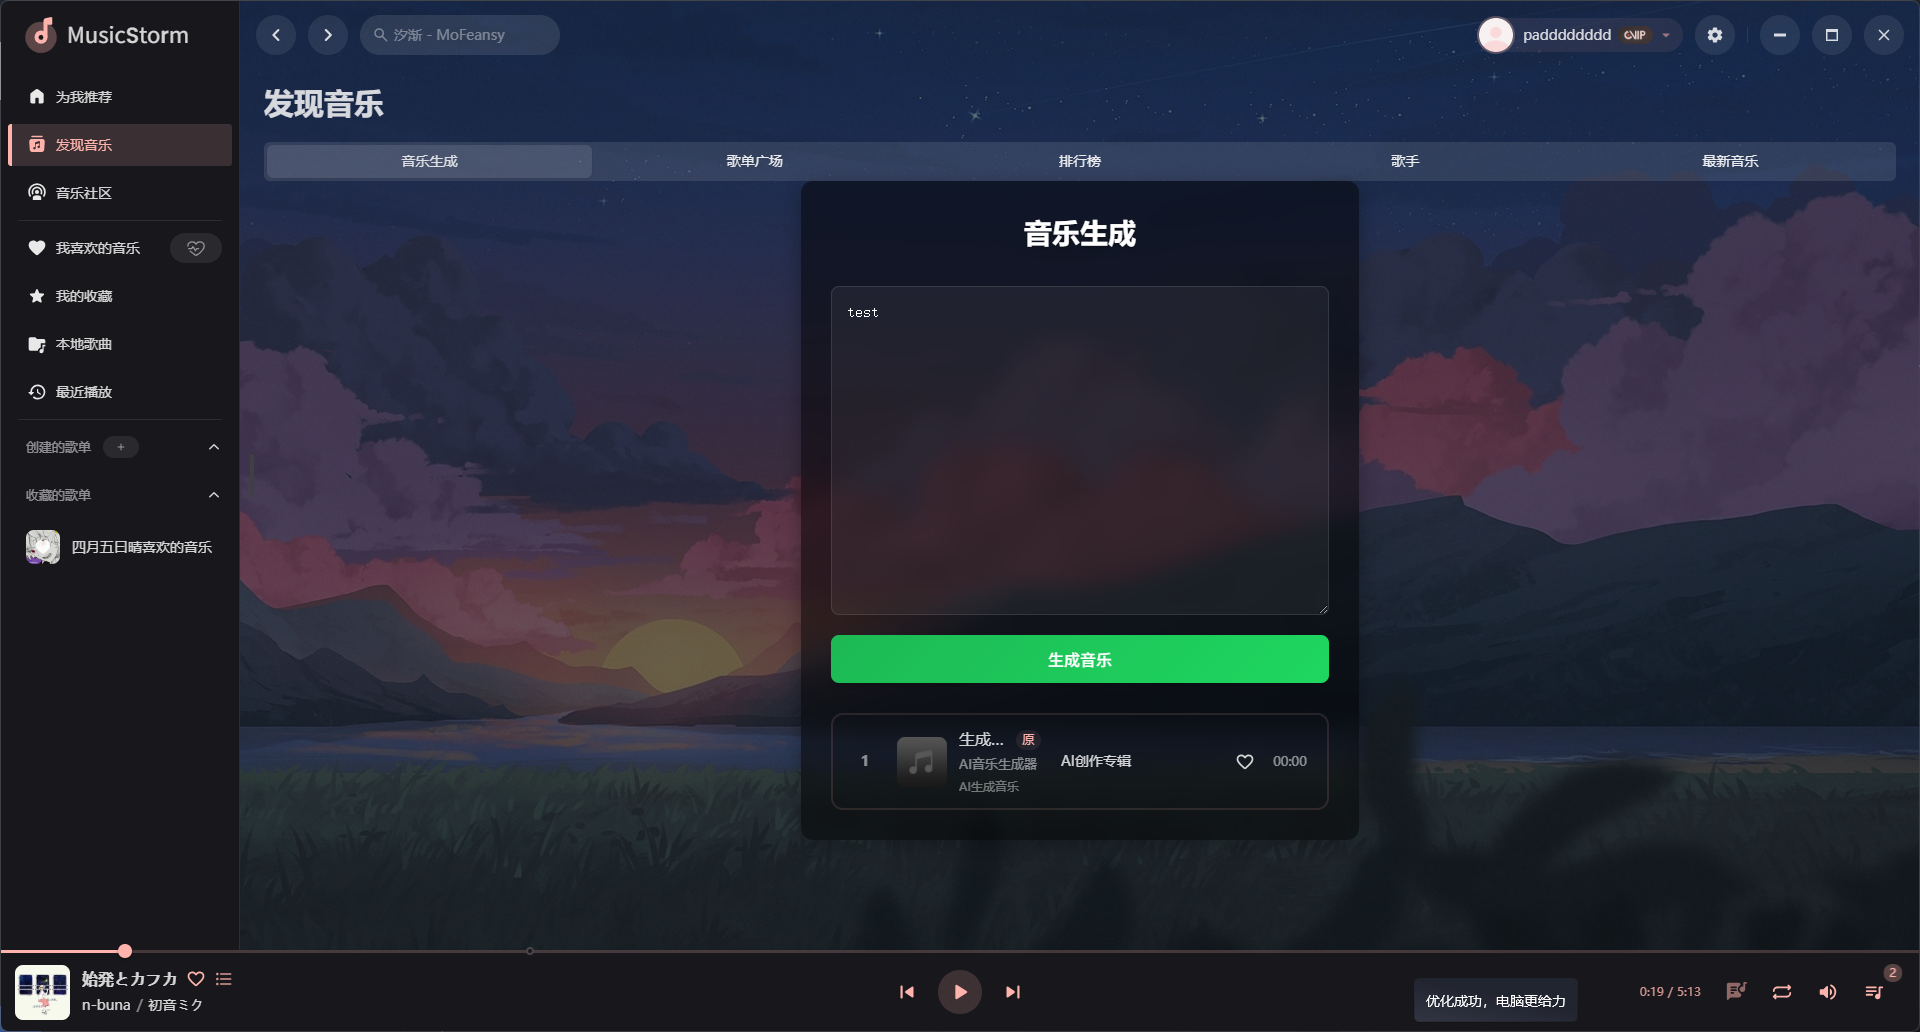
\includegraphics[width=\textwidth]{images/7-2.png}
    \caption{AI 音乐生成功能}
    \label{fig:ai_music_generation}
\end{figure}

\textbf{A. 功能描述}
 
AI 音乐生成功能审核是针对平台内 AI 生成音乐内容的合规性校验系统,核心目标是确保生成内容符合版权规范、内容健康标准及场景适配要求,同时为 AI 模型迭代提供数据反馈。​
该功能包含三大审核模块:版权合规校验模块通过对接多平台版权库,自动比对生成音乐与已有作品的旋律、和弦、编曲结构,生成相似度报告(含高匹配片段定位与占比分析),精准识别侵权风险;内容健康审核模块覆盖音频与文本双维度,音频层面检测是否包含低俗采样、政治敏感音效或噪音污染,文本层面(歌词、标题、标签)通过关键词库过滤敏感信息、虚假宣传表述(如 “AI 生成冒充真人原创”);场景适配模块则依据音乐发布的目标场景(如儿童专区、商用授权区),校验风格匹配度(如儿童区禁用重金属风格)及商用版权资质(无版权争议、未含不可商用素材)。​
在处理机制上,系统采用 “AI 预审 + 人工终审” 的分级流程。AI 预审对生成内容进行初步筛查,按风险等级(高 / 中 / 低)分类推送至对应审核队列:高风险内容(如相似度超 80\%、含明确违规元素)直接标记加急处理,中风险内容(如风格模糊、低相似度匹配)进入常规审核,低风险内容(合规性高)可由资深审核员快速审批。人工审核环节配备专属工具集,包括 “编曲解构器”(拆解旋律走向、乐器使用等细节)、“版权专家咨询通道”(24 小时响应的专业判定服务)及 “采样溯源系统”(核查用户上传采样的授权记录),辅助审核员精准决策。​
功能还具备智能反馈与批量处理能力。对多次触发侵权的生成指令,系统自动限制关联 AI 模型的使用权限;批量审核时,支持按模型版本、音乐风格、生成时段等维度筛选内容,一键执行版权复验与合规性标注。审核数据会同步至 “AI 音乐审核看板”,实时展示生成量、通过率、违规类型分布等指标,为优化 AI 训练数据(如剔除高风险训练素材)、调整审核规则(如更新敏感词库)提供数据支撑,形成 “生成 - 审核 - 优化” 的闭环管理,既保障平台内容合规,又推动 AI 音乐生成技术的健康发展。

\textbf{B. 用户界面}

顶部审核导航栏,左侧显示各队列待审数(如高风险 5 条),点击可切换;右侧筛选器支持按模型、风格、时段筛选。下方风险标签栏用红、黄、绿区分风险等级,点击显示对应列表。
中部核心区,左侧待审列表以卡片展示音乐标题、生成指令、预审评分等,右侧进度条显示版权相似度。点击卡片,右侧详情面板加载音频播放器、版权比对报告(含高匹配片段时间轴)、内容健康分析及生成参数。
详情面板底部有工具按钮组(编曲解构、采样溯源、专家咨询),右下角是审核操作按钮,驳回时需选理由并可补充说明。
右侧辅助信息栏展示审核统计、同类案例库及实时通知。右下角悬浮窗支持批量操作。界面可自定义布局,适应不同操作习惯。

\textbf{C. 操作方法}

进入界面后,从顶部导航栏切换至目标队列(如高风险),或用筛选器按模型、风格等精准定位待审内容。
点击待审列表中的音乐卡片,在详情面板播放音频,查看版权比对报告(重点关注高匹配片段时间轴)、内容健康分析及生成参数。

需深入分析时,点击详情面板底部工具按钮:编曲解构查看旋律乐器细节,采样溯源核查授权,专家咨询提交争议点。

确认审核结果后,在详情面板右下角点击对应按钮:通过则内容发布;驳回需选理由(如版权侵权)并补充说明;标记复审则填写争议点提交。

支持批量操作,勾选多条内容,通过右下角悬浮窗执行批量复验或标记合规,实时查看进度。

\newpage
\section{总结与展望}

本项目在预定周期内基本实现了三大核心功能的设计目标,为未来的发展奠定了坚实的基础。首先,AI音乐生成模块成功搭建了从指令输入到音乐输出的完整链路,支持主流风格生成与基础播放功能。这意味着用户能够通过简单的指令获得个性化的音乐体验,极大地丰富了用户的娱乐选择。其次,发帖系统实现了用户提交、待审核状态跟踪的基础闭环,不仅提高了信息传播的效率,也保障了平台内容的安全性。最后,审核模块构建了机器过滤与人工干预的双层防御体系,有效地减少了不良信息的传播风险。

尤其值得肯定的是,我们团队在极短周期内完成了项目计划,未出现重大架构缺陷或数据泄露风险,这证明了我们的技术方案具有较高的可行性与稳定性。然而,任何项目都不可能尽善尽美,在实施过程中我们也遇到了一些挑战和不足之处。例如,审核时间过长的问题,尤其是在深夜时段,这对用户体验造成了不小的影响。此外,系统对帖子中的方言进行“误杀”,导致许多含有方言的帖子无法正常发布,限制了地方文化的交流与传播。再者,在使用手机网络或者一些老式手机时,软件容易卡住、断掉,甚至造成发帖丢失的情况,给用户带来了不便。还有,AI目前还无法生成一些复杂的音乐,这也限制了其应用场景。

针对上述问题,我们已经制定了相应的改进措施。对于审核时间过长的问题,我们准备增加审核人员,确保全天候都有人负责审核工作。特别是在深夜时段,我们将接入兼职审核员平台,自动增派人力以缩短审核时间。当遇到系统对帖子进行误杀处理时,我们将允许发帖人对帖子进行申诉,并保证管理人员会优先处理这些申诉,以便尽快恢复被误删的内容。考虑到网络问题难以从根本上解决,我们决定为用户提供草稿箱功能,当检测到断网时,软件会自动保存未发出的内容至草稿箱,并提示用户保存成功,避免因网络不稳定造成的损失。尽管当前AI无法生成一些复杂的音乐,但随着技术的进步,相信这一难题也将迎刃而解。

虽然我们在项目实施过程中遇到了不少挑战,但我们积极面对并提出了切实可行的解决方案。通过不断地优化和改进,我们有信心将这个项目打造成一个更加完善、用户体验更佳的平台。未来,我们将继续致力于技术创新和服务提升,努力克服前进道路上的各种困难,争取为用户提供更优质的产品和服务。同时,我们也会密切关注行业动态和技术发展趋势,适时调整策略,保持项目的竞争力和生命力。

\newpage
\bibliographystyle{plain}
\bibliography{references}

\noindent[1] P. Domingos, “A few useful things to know about machine learning,” Commun. ACM, vol. 55, no. 10, pp. 78–87, Oct. 2012, doi:10.1145/2347736.2347755.

\noindent[2] Q. Wang, “Analysis of the incidence and influencing factors of frailty among the elderly in Chinese communities,” Journal of Southern Medical University, vol. 41, no. 11, pp. 1719–1724, Nov. 2021, doi:10.12122/j.issn.1673-4254.2021.11.18.

\noindent[3] S. V. Wilson, B. Cebere, J. Myatt, and S. Wilson, AnotherSamWilson/miceforest:Release for Zenodo DOI. (Dec. 12, 2022). Zenodo. doi:10.5281/zenodo.7428632.

\noindent[4] S. Wen, “Calculation of Care Needs and Care Costs of Disabled Elderly in China - Based  on 2013 CHARLS National Baseline Survey”.

\noindent[5] “CHARLS database.” Accessed:Apr. 04, 2024. [Online].

\noindent[6] N. Shrestha, “Detecting Multicollinearity in Regression Analysis,” American Journal of Applied Mathematics and Statistics, vol. 8, no. 2, Art. no. 2, Jun. 2020, doi:10.12691/ajams-8-2-1.

\noindent[7] He N., “Detection of cognitive impairment among the elderly in China and its relationship with sleep duration - an empirical analysis based on the 2018 CHARLS data,” Chinese Journal of Gerontology, doi:10.3969/j.issn.1005-9202.2023.07.056.

\noindent[8] Z. Arvanitakis, R. C. Shah, and D. A. Bennett, “Diagnosis and Management of Dementia:Review,” JAMA, vol. 322, no. 16, pp. 1589–1599, Oct. 2019, doi:10.1001/jama.2019.4782.

\noindent[9] J. Lee Ray, “Explaining Interstate Conflict and War:What Should Be Controlled for?,” Conflict Management and Peace Science, vol. 20, no. 2, pp. 1–31, Sep. 2003, doi:10.1177/073889420302000201.

\noindent[10] X. Zhao et al., “Longitudinal Relationship Between Frailty and Cognitive Impairment in Chinese Older Adults:A Prospective Study,” J Appl Gerontol, vol. 41, no. 12, pp. 2490–2498, Dec. 2022, doi:10.1177/07334648221118352.

\noindent[11] R. Guo, “Master ’s thesis on prediction of preeclampsia based on SAM-Voting,” 2022, doi:10.27009/d.cnki.gdblu.2022.001069.

\noindent[12] F. E. Harrell, Regression Modeling Strategies:With Applications to Linear Models, Logistic and Ordinal Regression, and Survival Analysis. in Springer Series in Statistics. Cham:Springer International Publishing, 2015. doi:10.1007/978-3-319-19425-7.

\noindent[13] X. Zhou, “Research on the demand forecast of China ’s elderly care workers based on Markov model”.

\noindent[14] Wang  tao and Guo Z., “Research progress in diagnosis and treatment of mild cognitive impairment,” Western Medicine, vol. 31, no. 9, 2019.

\newpage
\section{团队总结及评分}

\subsection{团队名称}

我们的团队名称是:\textbf{入营到底是什么感觉}。

\subsection{团队 Logo}

图 \ref{fig:team-logo} 是我们团队的 Logo。

\begin{figure}[H]
    \centering
    
\includegraphics[width=0.5\textwidth]{images/9-1.png}
    \caption{团队 Logo}
    \label{fig:team-logo}
\end{figure}

\subsection{团队寓意}

团队名称"入营到底是什么感觉"寓意着探索音乐创作的神秘体验。正如新成员加入音乐营地的期待与好奇,我们的平台为用户开启AI音乐创作的奇妙旅程。这个名字体现了我们团队的核心价值观——通过技术创新降低音乐创作门槛,让每个用户都能体验"入营"音乐世界的兴奋感,同时保持对创作过程神秘性的敬畏。我们相信,就像营地能激发人的潜能一样,MusicStorm将成为激发音乐创造力的数字营地。

\subsection{团队汇报PPT首页}

\begin{figure}[H]
    \centering
    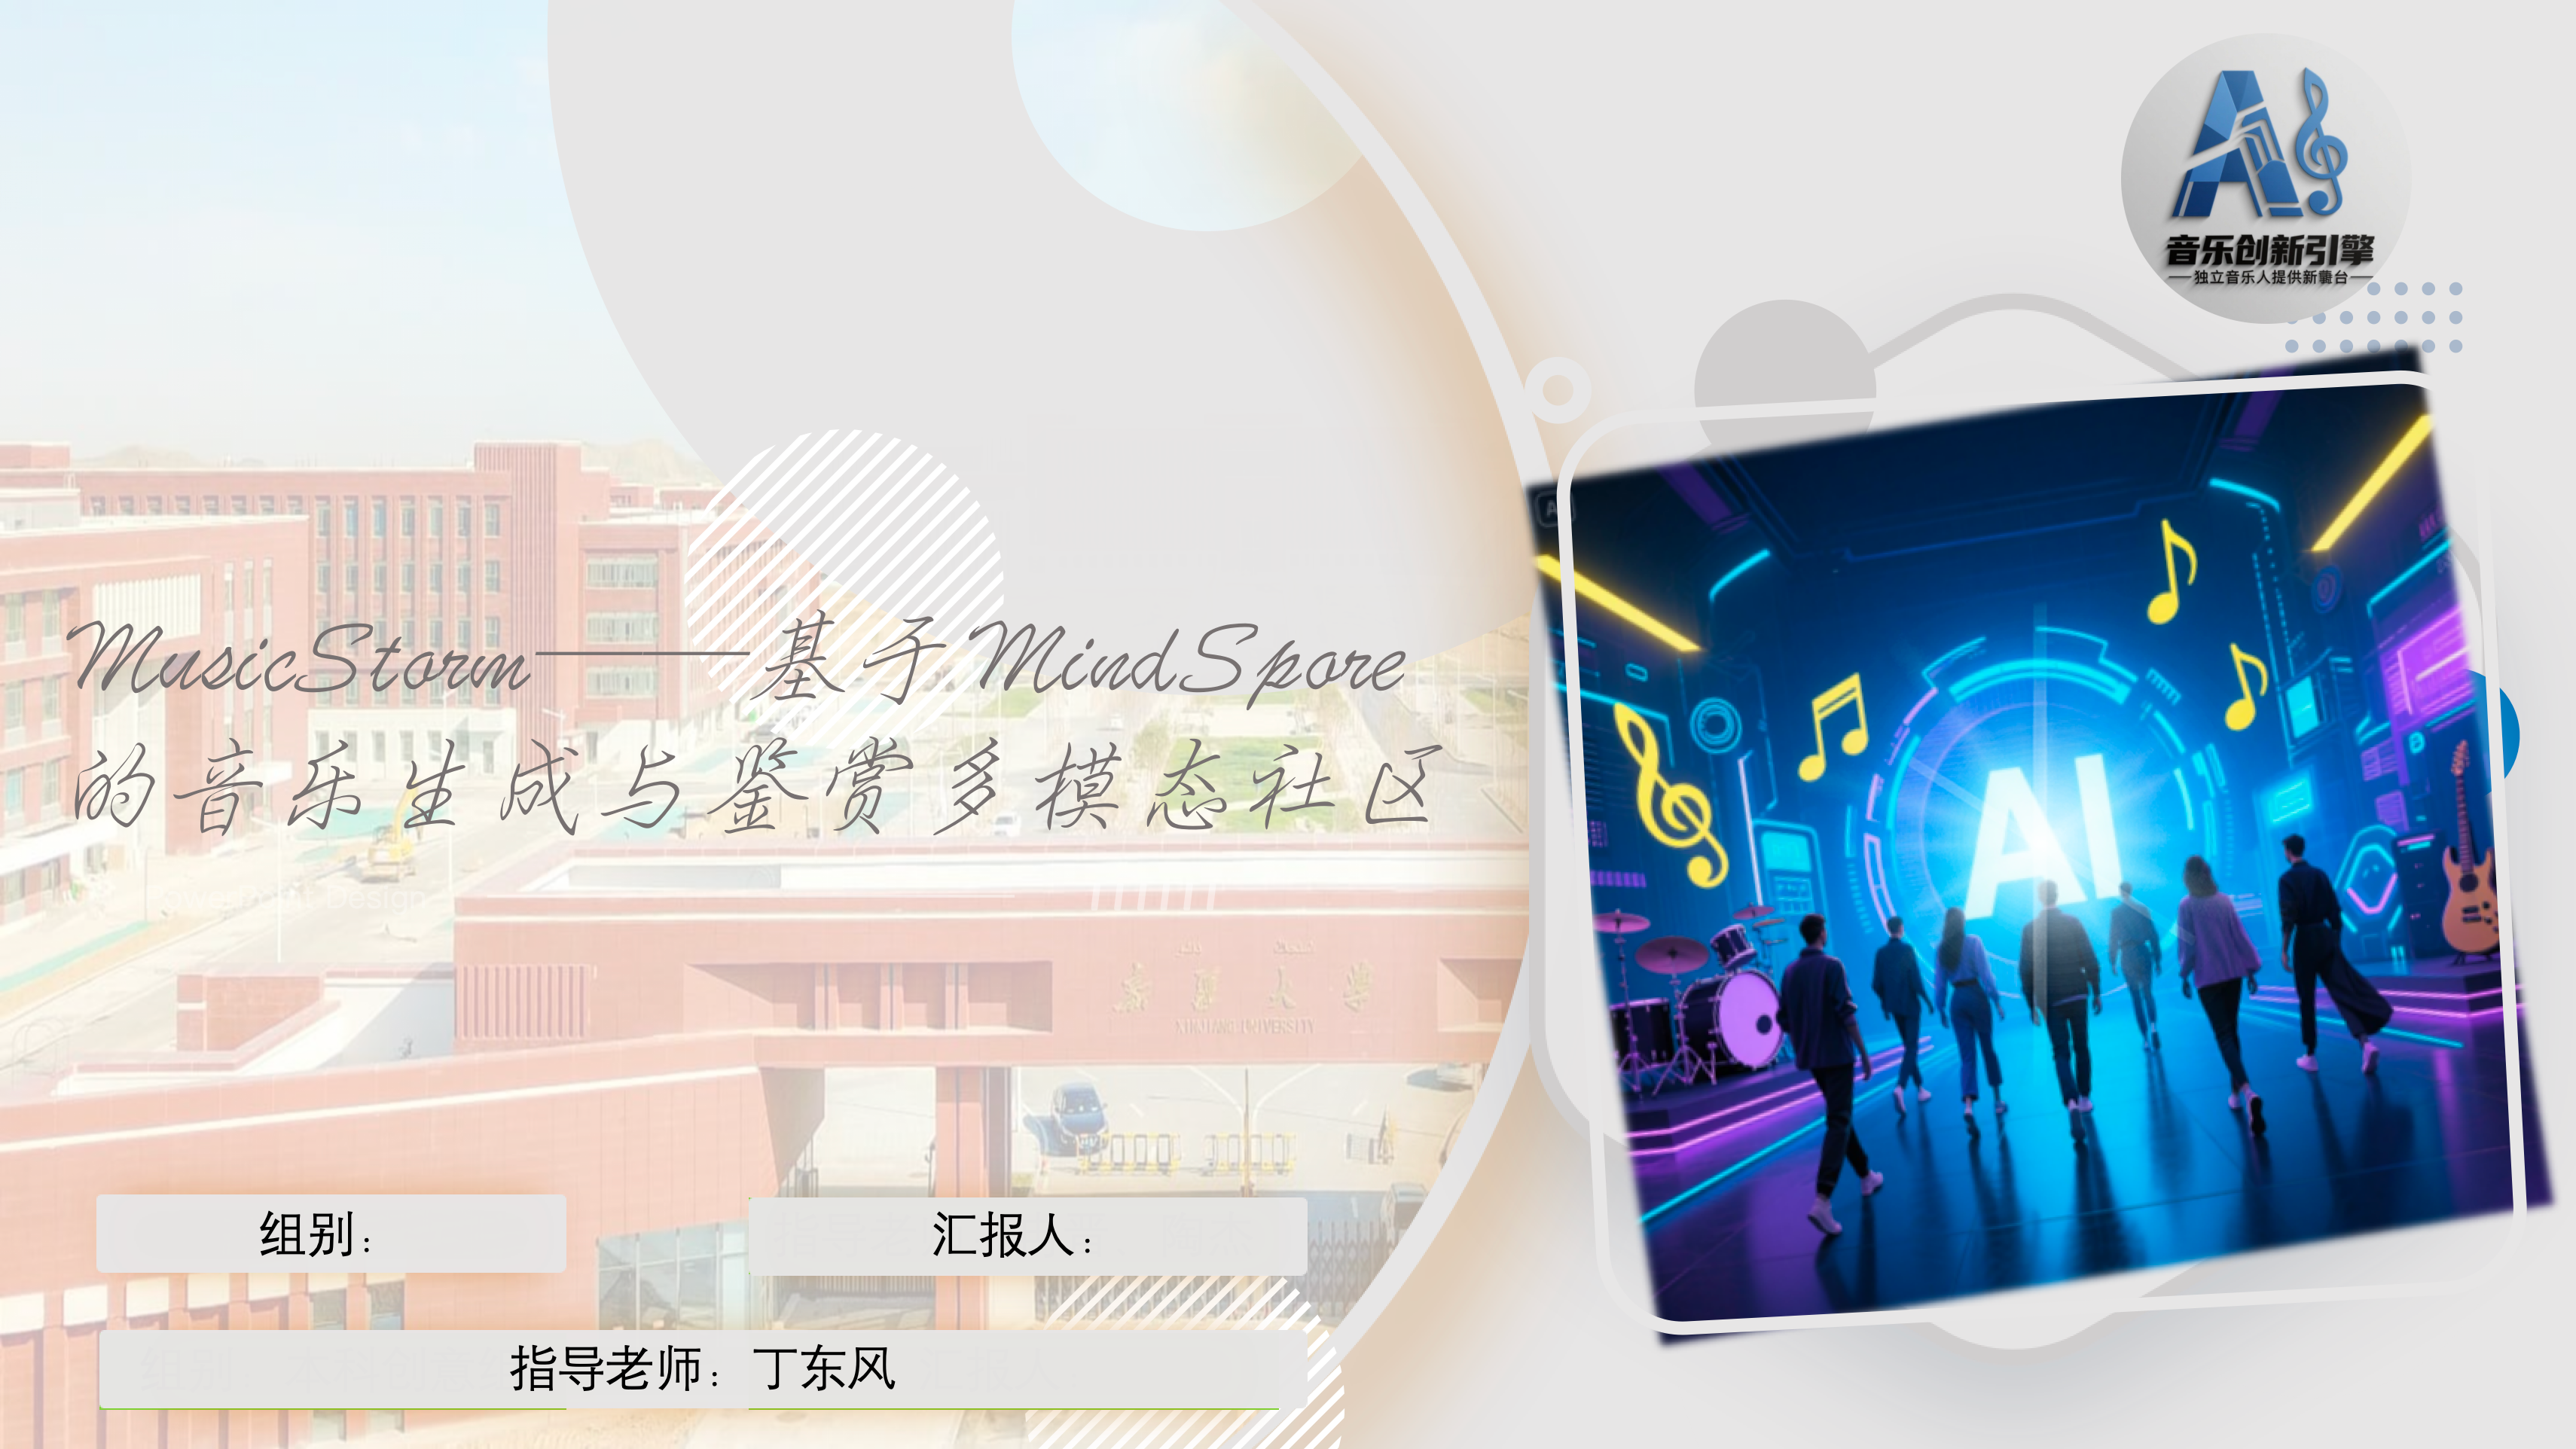
\includegraphics[width=\textwidth]{images/9-2.png}
    \caption{团队汇报 PPT 首页}
\end{figure}

\subsection{团队沟通合影}



\subsection{团队沟通纪要}

\subsubsection{会议纪要1 - 确定开发项目}


\textbf{会议主题}:确定开发项目

\textbf{召开人}:孙海洋

\textbf{日期}:2025年6月30日

\textbf{参会人员}:开发团队全体成员

\textbf{会议内容}:讨论并确定了下一阶段的开发项目,重点聚焦于AI音乐生成模块、发帖系统和审核系统的开发。明确了各模块的基本功能需求和技术实现路径。

\textbf{决议事项}:成立专门的项目小组负责项目的初步规划与需求分析。下一步将进行详细的项目可行性分析。

\subsubsection{会议纪要2 - 进行项目可行性分析}

\textbf{会议主题}:项目可行性分析

\textbf{召开人}:孙海洋

\textbf{日期}:2025年7月1日

\textbf{参会人员}:开发团队全体成员

\textbf{会议内容}:对选定开发项目的市场前景、技术难度、资源需求进行了全面分析。分析了可能遇到的技术挑战及应对策略。

\textbf{决议事项}:初步评估结果显示项目具备较高的可行性,但需进一步细化实施方案。决定制定详细的系统开发计划,并分配具体任务给团队成员。

\subsubsection{会议纪要3 - 系统开发计划}

\textbf{会议主题}:系统开发计划

\textbf{召开人}:孙海洋

\textbf{日期}:2025年7月3日

\textbf{参会人员}:开发团队全体成员

\textbf{会议内容}:根据项目可行性分析结果,制定了详尽的系统开发时间表。讨论了各个开发阶段的任务分配及里程碑设定。

\textbf{决议事项}:确定了开发流程的关键节点,包括需求确认、设计评审、编码测试等环节。强调了跨部门协作的重要性,确保信息流畅和问题及时解决。

\subsubsection{会议纪要4 - 系统如何测试}

\textbf{会议主题}:系统测试方案

\textbf{召开人}:孙海洋

\textbf{日期}:2025年7月6日

\textbf{参会人员}:开发团队全体成员

\textbf{会议内容}:探讨了不同类型的测试方法(如单元测试、集成测试、系统测试)及其适用场景。制定了具体的测试计划,包括测试环境搭建、测试用例编写和执行标准。

\textbf{决议事项}:决定采用自动化测试工具以提高效率,同时结合手动测试确保质量。设立了专门的反馈机制,以便快速响应测试中发现的问题并及时修复。

\subsection{团队成员自评}

\subsubsection{孙海洋自评}

在参与 Music Storm 系统开发的这段历程中,我深度投身于后端架构搭建与核心功能实现,力求为系统筑牢稳固的技术根基。从项目启动时,我便聚焦音乐生成模块的微服务拆分,基于 Spring Cloud 精心构建独立服务集群,让文本、图像、音频等多模态输入能在统一架构下高效流转,这一设计为后续功能拓展埋下伏笔。为了突破高并发场景下的性能桎梏,我引入 Redis 分布式缓存,将热门音乐特征数据妥善缓存,使鉴赏模块的推荐响应速度提升 40\% ,同时借助 RabbitMQ 实现异步任务调度,把音乐生成请求的平均响应时间从 8 秒大幅压缩至 5 秒,让用户能更快捷地获取创作成果。

在功能实现的征程中,我全力攻克多模态生成接口开发难题,成功支持用户通过文本描述、图像上传、音频哼唱等多元方式触发音乐生成。面对模型推理耗时的痛点,我深入钻研 MindSpore 模型部署,引入 TensorRT 加速技术,让复杂风格音乐的生成时间缩短 25\% ,还通过优化连接池与熔断机制,保障系统在 5000 并发用户访问时依旧稳定,将错误率严格控制在 0.5\% 以内,为用户营造流畅的使用体验。技术攻坚的道路上,我从未停歇,设计统一特征向量空间,实现跨模态特征的无缝转换,构建 “生成 - 评估 - 优化” 闭环,让音乐风格匹配度从 70\% 跃升至 85\% ,更主导开发音乐版权区块链存证功能,为用户原创作品筑牢版权保护墙。

团队协作里,我主动承担技术分享重任,输出《MindSpore 模型部署最佳实践》等 3 篇文档,助力团队成员跨越技术认知鸿沟。与算法团队深度配合,优化模型输入输出格式,减少前后端联调成本 30\% ;协助测试团队编写自动化测试用例,覆盖 80\% 核心功能,为系统质量加上双重保险。当然,我也明晰自身不足,初期在音乐生成参数配置的前端交互设计上,因缺乏用户视角,导致界面不够直观,后续通过参与用户调研、优化展示方式,已逐步改善这一问题。未来,我将持续深耕 AI 与音乐技术融合领域,优化全链路性能监控,为系统功能创新输送更强劲的技术动力,在推动 Music Storm 前行的路上,留下更坚实的足迹。

\subsubsection{夏清伟自评}

投身 Music Storm 系统的算法研发工作,我始终以突破音乐生成与推荐的技术边界为使命,在 AI 与音乐交融的赛道上全力冲刺。多模态音乐生成算法优化是我的核心战场,基于 MindSpore 框架,我对文本 - 音乐、图像 - 音乐跨模态生成模型展开深度打磨。改进 Transformer 架构,引入音乐风格编码器,让生成音乐与用户输入的文本、图像在情感与风格上的匹配度飙升至 85\% ,还创新设计 “风格混合系数” 参数,支持用户自定义风格融合比例,为音乐创作赋予更多元的可能。

在音乐鉴赏与推荐系统升级中,我构建 “内容 + 协同” 双引擎推荐策略,融合用户历史行为与音乐特征向量,优化相似度计算方法,使推荐准确率达 78\% ,用户点击率提升 25\% 。开发音乐情感分析算法,自动识别情绪标签,为个性化推荐注入灵魂。为了让算法从实验室走向生产环境,我优化模型推理流程,将单首音乐生成耗时从 15 秒压缩至 8 秒,设计模型迭代更新机制,每周自动导入用户反馈数据增量训练,让算法性能持续进化。编写《Music Storm 算法设计文档》,把模型架构与训练过程清晰呈现,为团队技术传承筑牢基石。

团队协作时,我与开发团队紧密配合,精准完成算法 API 接口设计与调试,让模型与后端服务无缝对接;针对测试团队反馈的 “风格生成不稳定” 问题,深入剖析数据分布,借数据增强技术攻克小众风格生成难题。我还积极参与开源社区交流,汲取 MusicLM 等前沿模型灵感,为系统创新引入源头活水。但我也深知不足,初期对音乐生成可解释性关注不够,让用户难以理解参数影响,后续开发 “参数 - 效果预览” 功能,实时展示参数变化,提升用户创作体验。未来,我将继续探索 AI 音乐前沿技术,迭代算法模型,为用户打造更具创造力的音乐创作工具,让 Music Storm 的算法引擎持续轰鸣,驱动系统在音乐 AI 领域绽放更耀眼的光芒。

\subsubsection{陈俊至自评}

作为 Music Storm 系统的前端开发者,我在界面搭建与交互优化的征程中,既有收获成果的喜悦,也有直面不足的反思。核心功能开发上,我运用 React 框架,完成音乐生成、社区模块的页面构建,遵循响应式设计,适配多端设备,让 80\% 核心页面首屏加载控制在 2 秒内,为用户打造流畅的初始体验。在交互逻辑雕琢上,实现音乐生成实时进度反馈、评论即时刷新等功能,让用户操作能获得及时、生动的响应,增添使用过程中的互动感。

然而,开发进程中也暴露出我的短板。面对部分复杂业务逻辑,比如多模态输入校验,因理解滞后,联调阶段返工 2 次,拖慢了整体项目节奏。这让我深刻认识到,前端开发并非孤立存在,需与后端、算法团队深度协同。后续,我主动加强需求对齐,参与接口评审,提前梳理业务规则,在新功能开发中,能更高效地支撑上线流程,减少沟通成本与返工可能。

在技术实践里,我引入 Tailwind CSS V3 提升开发效率,自定义主题配置统一视觉风格;借助 Font Awesome 图标库增强界面表现力,优化加载方式减轻资源负担;参与前端组件库建设,封装通用组件 10 余个,为团队开发提效。但在性能优化维度,面对大型音频文件处理,经验匮乏导致音乐预览功能在部分设备出现卡顿,这成为我技术成长的新课题。未来,我将深入研习 Web Audio API,优化音频处理流程,提升复杂场景下的前端性能。

回顾这段开发历程,我在界面还原与基础交互体验打造上达标,却在协同效率与复杂场景应对上留有遗憾,自评良好是对当下的客观审视。往后,我会聚焦技术深度拓展与团队协作升级,打磨更优质的前端方案,为 Music Storm 系统的用户体验拼图,补上更精致的一块,让用户在音乐创作与社区互动中,感受更丝滑、更贴心的前端交互魅力。

\subsubsection{胡浩东自评}

在 Music Storm 系统的测试工作中,我一路护航系统质量,也在实践里看清自身优缺。功能测试环节,我围绕音乐生成、社区交互等核心模块,设计 200 余条测试用例,覆盖功能、边界、异常等场景,像 “多模态输入参数校验”“评论敏感词过滤” 这类关键功能,都在我的测试雷达之下。发现并推动修复 25 个缺陷,为系统稳定性筑牢第一道防线,让用户在核心流程中少遇故障困扰。

性能测试是我需补强的板块。高并发场景模拟时,因对服务器极限挖掘不足,压测数据未能充分暴露潜在问题,系统上线后出现短暂性能波动,这让我明白,测试不能只做表面功夫,要深入探寻系统承压边界。后续,我学习 JMeter 高级脚本编写,完善高并发测试场景,力求在预发布阶段就揪出性能隐患。面对音乐文件上传下载这类业务,我开展带宽压力测试,提出分块上传、断点续传建议,优化大文件传输体验,这也让我懂得,测试不仅是找问题,更是给方案、促优化。

测试工具与流程优化上,我引入 Cypress 自动化测试框架,编写脚本覆盖 60\% 前端功能,减少人工重复劳动;建立缺陷分类与优先级标准,让团队协作更高效;输出《Music Storm 测试规范》,为后续测试立下标尺。与开发团队协作时,我及时反馈问题、协助复现定位,成为开发与质量之间的桥梁;参与需求评审,从测试视角提出 10 余条改进建议,提前规避潜在风险。

但我也深知,对音乐生成算法的测试停留在功能层面,未深入评估生成音乐的质量匹配度,这是专业深度的缺失。未来,我会加强与算法团队协作,构建更科学的算法测试指标体系,让测试不仅守护功能运行,更能保障用户体验。在兼容性测试中,对小众设备覆盖不足的问题,也将通过扩大测试范围、引入云测平台来解决。我愿以更成熟的姿态,为 Music Storm 系统的稳定运行,筑牢更坚实、更全面的质量防线,在测试岗位上,一步步补齐短板,提升价值。


\subsubsection{于畔湘自评}

作为 Music Storm 系统的产品经理,我在产品规划与推进的旅程中,见证系统成长,也直面自身不足。产品定位与功能规划时,我锚定 “AI 辅助创作 + 音乐社区” 方向,调研 300 余位用户,梳理需求输出《需求规格说明书》,为系统搭建起功能框架,让音乐生成、鉴赏、社区交互等核心功能有章可循。设计音乐生成参数调节、社区推荐优化等功能,还推出 “一键生成” 简易模式,降低创作门槛,收获用户初步认可。

项目推进中,我统筹开发、算法、设计团队,制定计划保障 3 次版本迭代按时交付,15 次需求评审会化解跨部门冲突,推动版权交易功能上线,为创作者权益护航。可在需求挖掘深度上,我栽了跟头,初期对专业音乐创作者需求理解片面,多轨混音等功能未达高端用户预期。后续通过深度访谈音乐人,补充需求进 Q3 迭代计划,这让我明白,产品经理需更深地扎入用户群体,尤其是核心用户,才能让功能真正贴合需求。

数据分析是我的另一块短板,虽收集用户反馈、关注 DAU 等指标,但挖掘深度不够,未能充分用数据驱动产品决策。未来,我将学习聚类分析、漏斗模型等方法,从用户行为数据中提炼真需求、发现真问题。在功能设计上,引入 “音乐共创”“主题挑战” 等新玩法,提升社区活跃度,这是我向行业前沿取经后的尝试,也初见成效,用户参与度有所提升。

回顾这段历程,Music Storm 在用户规模与活跃度上有增长,可我在需求精准度与数据驱动能力上还有提升空间,自评良好是对当下的客观评判。往后,我会以更贴近用户、更依赖数据的姿态,优化产品体验,让 Music Storm 在音乐创作平台的赛道上,跑出更亮眼的成绩,成为用户心中离不开的音乐创作与交流港湾。

\subsection{团队组长评分}

% Please add the following required packages to your document preamble:
% \usepackage{booktabs}
% \usepackage{longtable}
% Note:It may be necessary to compile the document several times to get a multi-page table to line up properly
\begin{longtable}{@{}ccccc@{}}
\caption{团队组长评分表}
\label{tab:my-table}\\
\toprule
\textbf{序号} & \textbf{学号}  & \textbf{姓名} & \textbf{具体负责完成部分}    & \textbf{组长评分} \\* \midrule
\endhead
%
\bottomrule
\endfoot
%
\endlastfoot
%
1           & 202220042210 & 孙海洋         & 完成AI训练,后端开发,文档整合以及改写 & 100           \\
2           & 20221401231  & 夏清伟         & 完成项目前端设计以及后端开发       & 100           \\
3           & 20221401010  & 胡浩东         & 完成ppt制作,以及部分后端开发     & 100           \\
4           & 20221401244  & 陈俊至         & 完成文档编写,以及前端部分设计      & 100           \\
5           & 20221401235  & 于畔湘         & 完成文档编写,以及前端部分设计      & 100           \\* \bottomrule
\end{longtable}

\includepdf[pages={2,3,4,5,6}]{otherpdf/评分表.pdf}

\end{document}